\documentclass[11pt]{book}
\usepackage[utf8]{inputenc}
\usepackage[T1]{fontenc}

\usepackage{Ambrosius}

%\usepackage{amsmath}
%\usepackage{amsfonts}
%\usepackage{amssymb}
%\usepackage[version=4]{mhchem}
%\usepackage{stmaryrd}
%\usepackage{graphicx}
\usepackage{relsize}
\usepackage[export]{adjustbox}
\graphicspath{ {./images/} }
\usepackage{hyperref}
\hypersetup{colorlinks=true, linkcolor=blue, filecolor=magenta, urlcolor=cyan,}
\urlstyle{same}

\let\origvarphi\varphi
\renewcommand*\varphi{\mathlarger\origvarphi}

\newcommand{\ols}[1]{\mskip.5\thinmuskip\overline{\mskip-.5\thinmuskip {#1} \mskip-.5\thinmuskip}\mskip.5\thinmuskip} % overline short
\newcommand{\olsi}[1]{\,\overline{\!{#1}}} % overline short italic

\newcommand\vecur[1]{\setbox0=\hbox{$#1$}\lower1ex\hbox to 0pt{\hbox to \wd0{\hss$\rightarrow\;$\hss}\hss}\box0}
\newcommand\vecul[1]{\setbox0=\hbox{$#1$}\lower1ex\hbox to 0pt{\hbox to \wd0{\hss$\leftarrow\;$\hss}\hss}\box0}

\newcommand\kcmd[1]{{\tt \textquotesingle #1\textquotesingle}}

% Book size changed to 7 by 10
\geometry{paperwidth=7in,paperheight=10in,textheight=8in,top=1.1 in,left=0.66in,right=0.66in,bindingoffset=5mm,twoside}

\title{PhD Thesis:\\
 Studies on complex enzyme systems\\ \phantom{a}\\

{\Large Thesis presented for the Degree of Doctor of Philosophy of
the University of Edinburgh in the Faculty of Science.
May, 1971.}}

\author{Jim Burns}
\date{\large Transcribed to \LaTeX\ by Herbert M. Sauro February, 2023, based on a photocopy of the thesis obtained in 1988.}

\begin{document}

\maketitle

\tableofcontents


\renewcommand*{\thesection}{\Roman{section}.}
\renewcommand*{\thesubsection}{\arabic{section}.\arabic{subsection}}

\chapter*{Introduction}
\markboth{\bf INTRODUCTION}{}

Advances in biochemistry and molecular genetics have been concerned with gene action, protein synthesis, and protein structure. Thus we now have a fairly detailed picture of how protein structures are determined, both as regards specific configuration and as regards the mechanism and energetics of their syntheses. Furthermore by a combination of genetic and biochemical investigations in the area usually described as `metabolism' we are obtaining an ever widening picture of the relationships between metabolic steps, often displayed as metabolic maps which show in a qualitative way the flow of synthetic and degradative pathways (anabolism and catabolism). Although this picture is by no means complete there is a general feeling that the major structure of living systems, at this level, is known. Broadly speaking the genetic specification, i.e. the base sequence of the DNA, determines the parameters (quantity, turnover numbers and Michaelis constants) of the enzymes which catalyse the biochemical transformations of the metabolic network. What is much less understood, however, is how such specifications affect the quantitative outcome of the multiple interactions within a metabolic system which, in the end, determines the measurable properties of the whole system or organism. What is, therefore, required is a "quantitative biochemistry" as well as the relation of this to quantitative genetics, whose approach has been both historically and methodologically quite different from molecular genetics. This thesis is an attempt to relate the three fields of molecular genetics, metabolic biochemistry and quantitative genetics.

\section{Non-quantitative nature of present system theory}

During the past few decades the joint application of genetics and biochemistry to relatively simple organisms such as viruses, bacteria and syncytia has led to an increasing elucidation of their details. There has been great success in discovering system components, isolating them from homogenates, studying their properties in vitro and defining their relationship to the complete system. We now possess a fairly universal classification of system components into such types as genes, messenger RNA, ribosomes, proteins and a knowledge of their respective functions within the cell. The detailed action of these subunits may vary across strains and species but at least at the level of cell biology the general picture is fairly clear. For some types of organism such as E.coli, yeast and Neurospora a great deal is already known. Thus it is claimed that about $40 \%$ of all metabolic activity has been accounted for in {\em E. coli} K12 (J.D. Watson, 1965).

It seems then that, as this detail is added to, we shall, at the level of cell biology, be increasingly in the situation of, viewing the organism in terms of a sort of chemical engineer's block diagram. The engineer's blocks now represent the separate genetically specified transformational activities (enzyme catalysis) taking place in metabolism and the engineer's system variables become the various chemical concentrations being transformed one to another in the cell. Indeed, the cell has been viewed in just this way for a long time, the great achievement being to define and characterise what all the separate `blocks' are. Thus a large class of data is explained for a given cell type by a transformational block diagram, tentatively proposed for that cell. Such data is essentially qualitative such as, for example, whether a given enzymic activity is present or absent in the extract of a mutant or whether the mutant can grow or not on a minimal medium with a certain supplement. The block diagram explains the data insofar as it allows qualitative prediction of the effects. of hypothesised large changes to blocks within the diagram.

Thus we have a reasonably well established `qualitative system theory' of cell metabolism which is consistent with a large body of qualitative date and this theory is similar in general outline over a wide range of cell types.

More recently there has been considerable interest in extending transformational diagrams by adding to them a `control level' showing which system variables have a strong effect on the rate of any given transformation, although in this case the details have been found to vary considerably over different cell types. These studies have involved the consideration of a less qualitative type of data, for example, the measurement of low, intermediate and high levels of an enzyme in extracts of cells grown under various conditions. Nevertheless, even with the inclusion of a control level, the present system theory of cell metabolism has remained essentially qualitative in nature. Unlike the engineer, the biologist is not at present easily able to use his block diagram to predict the quantitative effects of substituting a slightly altered form of one of his blocks (enzymes) or of altering the level of an external metabolite.

What will be the form of a quantitative theory? Clearly with the existing system theory one worked from a block diagram, itself constituting the theory, and used a form of logical argument to predict the consequences of any particular lesion. With a quantitative approach it will be necessary to attach to each block in the diagram a formula of some sort giving the rate of its transformational activity. This formula being in terms of the system variables which strongly affect the block and of the genetically specified parameters which describe it.

Although any change in a block or environmental parameter will directly affect the rates of only a few activities these will affect system variables which will affect other activities and so on. The quantitative response of any system property is thus the result of a complex balance between the various activities underlying the system. In a quantitative theory prediction will thus require a calculation which allows fully for the detailed behaviour of the separate blocks as well as for the block diagram which was sufficient for a qualitative theory.

Just as the qualitative system theory aimed to explain a wide range of qualitative data, so any quantitative extension must now include a much larger body of quantitative data which, although it may not conflict with the transformational and control diagram, is by no means explained by it.

\section{Some quantitative approaches}

I shall consider first some studies which have avoided explanation of particular data and have asked instead what general properties may arise out of commonly occurring metabolic mechanisms. Thus Goodwin (1963) focussed attention on possible dynamic consequences of the feedback loops found to control enzyme quantity in a variety of cells, conjecturing that they may be in a state of spontaneous oscillation. He has further considered cellular dynamics from the point of view of there being a number of such oscillators, weakly coupled, within each cell and treated this by the methods of statistical mechanics.

Following on this and also because of the clear experimental findings concerning metabolic oscillation there has been considerable discussion of the conditions under which such oscillations could occur. J.S. Griffiths (1968a, 1968b) has considered oscillators of the Goodwin type and defined more clearly the necessary conditions, his work suggesting that rather special assumptions are required. The problem of stability has also been considered by C. Walter (1968a, 1968b). A more abstract treatment is offered by S.A. Kauffman (1969) who has considered the cell as a system in which genes have only two states, on and off, the state of a gene in the next instant of time being determined by the state of a small number of genes controlling it at the previous instant. This abstraction of a problem, not unlike Goodwin's coupled oscillators, has enabled him to consider large networks with extensive coupling and to demonstrate that a number of interesting properties are possessed by such systems. Thus it appears that a network of `genes' connected at random and with randomly assigned boolean response function to their inputs will for the case where each gene has two inputs, almost always possess only a few distinct cycles of activity into which it rapidly falls when released from an arbitrary initial condition. Furthermore these cycles of activity are surprisingly short, involving often only a very few `states' of the system before repeating. This simple cyclic or even steady state behaviour is of some interest arising as it does in systems which at first sight might be expected to generate extremely complex dynamical behaviour. A further value of Kauffman's approach is that he relates cell metabolic theory to the already much studied theory of `finite automata'.

These approaches are, however, highly abstracted formulations remote from quantitatively ascertainable data and are, therefore, not suitable to make the link between the areas with which this thesis is concerned. More relevant to our purposes are the classical biochemical approaches as follows.

\section{Enzyme kinetics}

Here there exists an extensive literature, see for example "The Enzymes" (1959), the bulk of which is concerned with studies, both theoretical and experimental, on single enzymes. The basis of these studies is usually that the enzyme can exist as a number of alternative `complexes' with its substrates, products and inhibitors and that interconversion between these is governed by the usual chemical law of mass-action.

This gives rise to a set of 1'st order differential equations involving a number of hypothetical enzymic intermediates and the necessary rate constants to describe their mass-action interconversions. The data to which this theory is related is largely derived from {\em in vitro} studies, preferably with purified enzymes, and consists of the concentrations of substrates, products, and other substances at various times after the introduction of the enzyme. Only rarely is the concentration of an enzymic intermediate monitored directly and again the early rapid reaction phase is not normally observed. Consequently for most metabolic enzymes complicated kinetic schemes should be viewed with suspicion as also their rate constants, particularly when one considers that the conditions in vivo may be very different from that of the purified enzyme in isolation.

\section{Steady state enzyme kinetics}

This considers the situation when substrates and products are held at a steady concentration and asks what is their respective rate of removal or production by the enzyme. Bimolecular reactions are usually considered to take place only between enzymic intermediates and metabolites, protein interactions not normally being included. Under these circumstances a set of simultaneous equations can be written down which define the steady state levels of the various enzymic complexes and since these equations are linear in terms of the enzyme complexes it is possible to solve them explicitly. This yields the overall `rate' of the reaction as an algebraic expression involving the steady levels of the metabolites and the various rate constants characteristic of the protein. King and Altman (1956) have provided an elegant method for writing down the `rate expression' directly from a diagram of the kinetic scheme. The results of applying this systematically to a variety of kinetic schemes has been presented by W.W. Cleland (1963) who also advocates that the expressions be written using Michaelis constants and other enzyme kinetic constants which can be defined operationally, rather than with elementary rate constants. The simplest expression appearing in Cleland's paper being for the well known case of an enzyme catalysed reaction having one substrate and one product (H.L. Segal, 1959), when the rate expression takes the form
%
$$
\mathrm{FLUX}=\frac{\mathrm{ET} / M\left(S_{1}-S_{2} / K_{E}\right)}{1+S_{1} / M+S_{2} / M}.
$$
%
where $E$ is the concentration of the enzyme.

Here $M, M$ are Michaelis constants which are usually obtained directly from an assay for the forward and reverse reactions respectively as could $T$ the turnover number corresponding to `maximum velocity' in the forward direction. $K_{E}$ is the equilibrium constant for the reaction $S_{1} \rightarrow S_{2}$ This equation reduces to the well known rate expression due to Briggs \& Haldane (1925) when $S_{2}$ is set at zero.

This flux is a good approximation to the instantaneous value, even when the pools are varying slowly (Richards and Pring, 1968). We shall make use of equations of this type in later chapters. The rate expressions for even slightly more complicated kinetic schemes can become very cumbersome. Consequently several workers, for example R.O. Harst (1968) have resorted to programming the King Altmann method so that these more complicated rate equations can be produced automatically on a digital computer from a description of their kinetic schemes.

\section{Multi-Enzyme systems}

Perhaps the most consistent attempt at a quantitative treatment of a specific multi-enzyme system has been in relation to the glycolytic pathway, started by Chance in 1951. Since that time B. Chance, D.Garfinkel, J. Higgins and other workers have continued to develop experimental, theoretical and computer techniques - recently reviewed by D. Garfinkel (1970). Their reason for becoming involved in computer techniques is that the mathematical representation of even a simplified multi-enzyme system involves a large number of non-linear differential equations which cannot be handled by existing analytic techniques and have consequently to be solved by `simulation' on a digital or analogue computer. Their main interest has been in a study of the transient effects in the glycolytic pathway based on work with mouse ascites cells (B. Chance et al., 1960) and with heart and liver, (Garfinkel et al. 1968).

Long computation times are found in these systems, mainly due to the commonly encountered situation that the molar concentration of enzymic intermediates is much lower than that of metabolic intermediates. This produces high frequency components in the D.E. and the step length of the numerical integration procedure used has to be sufficiently small to cope with these. As a result considerable amounts of computer time can easily be expended in representing only a little `real' time in the biochemical system (Garfinkel, 1965).

Consequently an effort has been made to improve the methods of integration employed in simulation programmes so that they are more suitable for handling the `stiff' equations commonly encountered (Cooper, 1970). Recently (Curtis, A., unpublished data, 1970) the predictor-corrector method of Gear (1968) has been employed on a simulation problem, previously run using the method of E. Chance (1969), with a claimed improvement in speed of 100 times.

Another approach to the problem of computer efficiency has been to use the rate-equations of steady state enzyme kinetics which were discussed earlier, thus removing the differential equations corresponding to enzymic intermediates, which are mainly responsible for the stiffness encountered in biochemical systems. These rate equation representations are now, of course, only an approximation to the `true' dynamics but this will not normally be a serious discrepancy (Rhoads and Pring, 1968).

A problem which has received considerable attention is that of how to `describe' the biochemical system to the computer and the more recent programs of Gerfinkel (1968) and of E. Chance (1969) will accept a form of biochemical-language which is meaningful to the experimental biochemist. For programmes employing mainly rate-equation methods the use of a biochemical language is not so straightforward but, (Rhoads and Pring, 1968), methods have been devised to generita these automatically and link them into the commonly employed simulator programs (Garfínkel, 1968).

Some unexpected results have arisen on the experimental side. Thus Chance et al. (1964) find sustained oscillations, apparently arising at the level of intermediary metabolism. This has stimulated theorist's, as for example Achs and Garfinkel (1968) to construct oscillatory models. Again Garfinkel (1969) remarks that very few enzymes, working in situ, behave as they do in isolation.

All of the quantitative work just mentioned assumes implicitly that the cell can be regarded as chemically homogeneous or `well mixed', although it is possible to include a limited type of inhomogeneity.

\section{The problem}

The purpose of this thesis is to develop a suitable theoretical framework together with relevant computer techniques, which it is hoped will illuminate the beheviour of genetical systems. By genetical systems is meant an organism (or its analogue) or a population of organisms which is specified by a set of initial parameters (genes and environment) and into which we can introduce variation. Such variation will be introduced either by considering alternative functional alleles at one or more genetic loci, or by changes in the environment.

An alternative allele will be represented by a quantitative change in the specification of a catalytically active molecular species (enzyme) while the environmental variation will be represented by a quantitative change in the concentration of one or more external sources of metabolites.

The essence of genetic methodology is the measurement of difference between organisms or populations. Which measurements are taken is arbitrary, but an analysis of systemic behaviour requires that the functional dependence of any measure is analysed in terms of the effect of the imposed variation on the system. our task, therefore, is to investigate how a metabolically organised system responds to variation in the parameters. which define it.

The measures in which we are interested are mainly time independent averages of some sort and are usually of a biochemical nature. Some examples would be concentration of a metabolite, quantity of an enzyme in a cell, net-flux in a metabolic pathway. The averages being obtained by sampling from a large exponential growing population, of asynchronous cells, from a single syncytium in exponential growth or from particular tissues of adult metazoa. Consequently we can argue (Chapter I) that a suitably extended `steady state' treatment of metabolism is the appropriate development from qualitative system theory. This steady state treatment must, however, include bimolecularity, inhibition of enzyme activity, repression and induction of enzyme quantity, saturation properties of enzymic reactions, and networks of arbitrary complexity since these are essential aspects of any real system and cannot be ignored without sacrificing important features of quantitative behaviour. It should be stressed that although much has been written on the theory of the steady state this literature has dealt almost exclusively with `linear' systems leaving out of consideration the non-linear phenomena mentioned above.

\begin{figure}
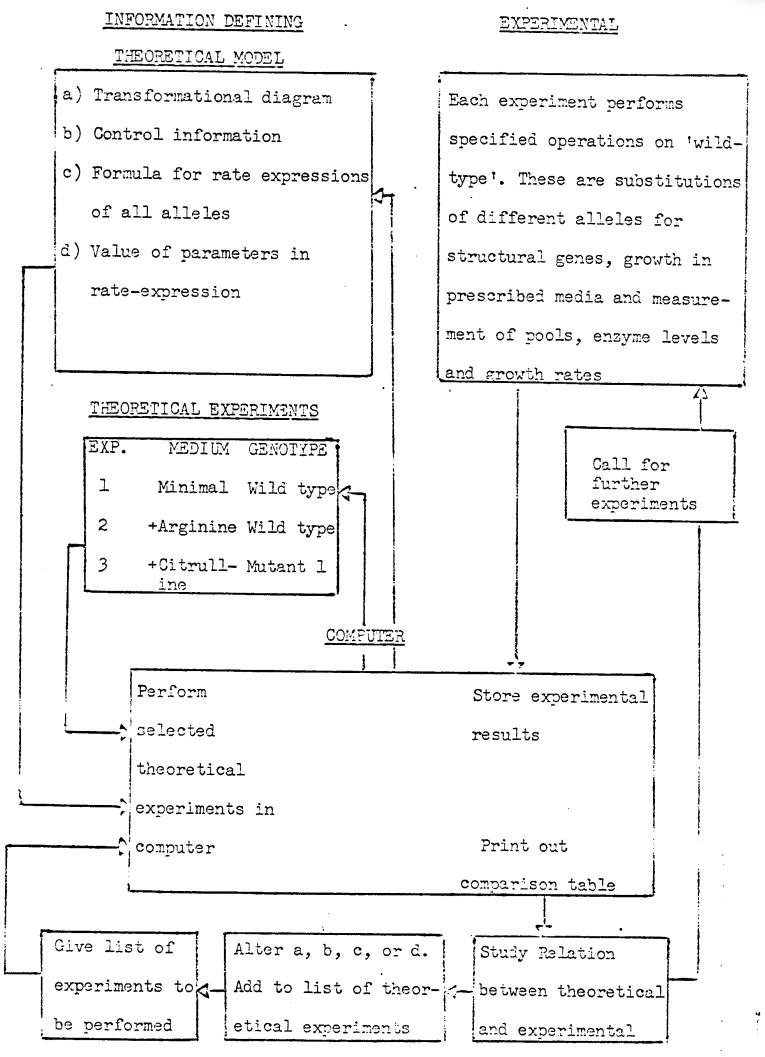
\includegraphics[scale = 1]{figure0_1.png}
\end{figure}

\section{Role of computer in relation to quantitative experiments}

Let us consider how one would set about establishing such a quantitative model within an area of metabolism where the block structure and the control structure has been tentatively established by means of qualitative information.

I have in mind particularly the sort of work which is being carried out in laboratories studying pathways in structurally simple organisms, but it is by no means restricted to these. Essentially the procedure is to measure a number of system variables, metabolic pools, enzyme levels, flux in pathway, both for the wild type organism and for strains with various quantitatively altered forms of enzymes. These `quantitative' mutants may be obtained as revertants from known mutants, affecting structural loci, which abolished enzyme activity, or may be discovered as natural variants. Measurements are taken both on minimal medium and on medium containing various supplements.

Thus a fairly large amount of data is gathered to which the proposed quantitative model must conform. In addition there will be some rough information, gained from in vitro studies, atout rate expressions for the wild type and mutant enzymes which will be helpful in formulating the initial theoretical model. Similarly, this kind of information may become available from natural or domestic animal populations. The facing diagram indicates an example of the necessary procedure.

There are several interesting features of this process which should be noted. Firstly, it can be seen that the computer plays an essential role. Without it the theoretical model could not be evaluated against the facts. Secondly, the process is not to be thought of as simply adjusting the parameters of a fixed model to fit the data by, for instance, hill climbing on some least squares procedure. Rather the process is more `scientific' than `statistical'. Thus not only the parameters but also the block diagram, the assumptions about control or the form of the rate expressions are all subject to alteration as the model is studied in relation to data.

A good example of this scientific situation and of the integral role of the computer is that the computer can be used to decide a quantitative question that of ten arises. Which of several experiments is likely to discriminate most sharply between currently competing hypotheses about the model?

Thirdly, it seems that the building up of a quantitative model is a more interactive process than was that for the qualitative model. Thus when we adjust our assumption about one part of the model to meet some new experiments we may disturb existing agreement with previous experiments. The computer is again invaluable here as it enables us to retest agreement with all previous experiments every time we adjust the model.

If this process of interaction between biological data and computer model proves successful the result would be twofold:

(1) We would be in possession of a model which consistently reflects the qualitative and quantitative results of the experimental data. This means that our confidence in having the "correct" model is strengthened. (2) We would have at our disposal a predictive tool which enables us to investigate novel situations which are either difficult, lengthy, or expensive to perform on biological material. This process is usually described as `simulation' and forms the goal of many investigations (and has been successfully applied in many fields of engineering). In the next section we shall argue, however, that this may fail on grounds of feasibility and, more importantly, that the general properties of quantitative systems may be used to answer questions of theoretical importance beyond the problem of the simulation of a particular organism (Kacser and Burns, 1968).

\section{General strategy for quantitative approach.}

At this point we must take stock of the general position in which quantitative cell metabolism is at the moment.

Firstly, if the aim is the setting up of an exact-quantitative model of metabolism in some cell type, we must first argue the value of having such a model. Often the effort required to establish the model will be out of all proportion to its value. Secondly, the feasibility of setting up a \underline{comprehensive} model of metabolism is doubtful at the present time, even for E.\ coli and certainly for all other cell types. Thus in most cases not even the necessary qualitative knowledge has been obtained. A more fundamental reason, however, is for instance, that the form of the rate expression of many enzymes, even in vitro, is still controversial and appears likely to remain so.

The strategy advocated here is that we should concentrate on acquiring the ability to incorporate quantitative information into a predominantly qualitative picture, and not to worry too much about details. As the need and opportunity arises this ability can be applied to various situations. Clearly just as the block diagram has been gradually extended over a period of many years so a qualitative model can gradually be turned into a quantitative model as the necessary reliable data on system disturbance and system response becomes available.

\section{Theoretical treatment of metabolic systems}

We have above painted a rather gloomy picture of the immediate prospects for a comprehensive quantitative approach based on real data and have also questioned its general usefulness, whilst pointing out the relation of computational and theoretical techniques to it.

However the same techniques can, just as easily, be applied to the construction and investigation, either by analysis or numerical exploration, of abstract metabolic systems expressed in the form of mathematical models. These abstract systems being chosen to posses structure, mechanisms and parametric values which are broadly similar to those of real systems. Many features of the quantitative response of real systems to parametric variation are not critically dependant on the exact parametric values obtaining. Such features, including the common occurrence of intra and inter locus interaction, the remarkable buffering ability against parametric change (Kacser, 1963) and so on, clearly arise mainly from the overall structure of the system rather than its precise parametric values. Accordingly we shall argue that it is legitimate to study such quantitative features, of systemic response to parametric variation, for suitably chosen abstract systems per se and this is in fact a major aspect of the thesis.

In principle this can be done by the numerical investigation of a wide variety of abstract systems over a wide variety of parameter values but in practice such {\em in numero} experiments are seldom informative (A. Robertson, 1967) owing to the large number of parameters involved in even the simplest model. Because of this considerable attention has been paid, whenever possible, to the algebraic investigation of system behaviour, both in a general way and, in more detail, for simple systems such as a chain of enzymes. In these studies it has proved useful to introduce the `sensitivity coefficient' (Kacser and Burns, 1968; Burns, 1968) as an index of response and to show how these coefficients are related to the quantitative behaviour of the individual parts of a system. The theoretical properties of these coefficients can then be used to discuss features of parametric response, such as `buffering', in a general way. A similar coefficient has been used by J. Higgins (1963) although in a somewhat different context.

Arising from such a treatment it may be possible to consider populations of biochemical systems which differ from each other in many parameters. This is the implicit assumption of quantitative genetics, but the usual theoretical method (e.g. Fraser, 1962, 1967) of handling metric characters in population problems has been to set up arbitrary genotype-phenotype relationships. A quantitative biochemical treatment, however, considerably restricts and defines the relationships insofar as `additivity', `epistasis', and `dominance' must not be postulated but will (or will not) arise from the underlying metabolic structure of the organisms. We shall consider a number of aspects in this manner for a simple abstract system and will suggest methods for investigating more complex systems by numerical means (Burns, 1970). 
\renewcommand*{\thesection}{\arabic{section}.}

\chapter{Real Organisms and the Choice of Kinetic Systems}
\markboth{REAL ORGANISMS}{}

In the introduction it was stated that a major aim would be to provide a suitable theoretical framework, in which to consider how variability in an organism at the genetic (or information storage) level will be expressed at the level of measurements made on the `system' which is the organism. The purpose of this chapter is to show precisely what is meant by this, to provide such a framework, to consider properties of unimolecular systems in relation to it and finally to introduce a number of general concepts in connection with these systems. In Chapter II consideration will be given to the formulation, within this scheme, of more complex metabolic systems which can more reasonably stand as analogues for real organisms.

Before proceeding to consider specific types of systems it is important to make clear the general point of view which is to be adopted. Genes act by specifying the precise properties of functional units, usually proteins, which themselves act in many cases by catalysing specific reactions within a metabolic network of some sort. Accordingly many aspects of the general gene-action problem will be reflected in a more limited and abstract problem, namely that of how enzymes interact within a multi-enzyme system to determine measurable properties of the system, as for example the concentration of a given metabolite or the metabolic flux at a point in the network. Whilst no apology will be made for this abstraction from the general problem, the genetic systems to which the limited treatment is most relevant will clearly be simple unicellular or synctial organisms growing in a well defined culture medium. For complex multicellular organisms in a complex environment it will be less obviously relevant, although even here it may be applicable to the more biochemical type of character.

Given then that a first attempt to understand something of the quantitative aspects of gene action may be reasonably limited to a consideration of multi-enzyme systems, two further tactical questions arise. The first of these is concerned with the quantitative importance of the spatial organisation of metabolism within the cell. There is ample evidence that such organisation occurs, as for example at the high level of cell organelles such as mitochondria, and, at a lower level, where it has been suggested that several enzymes in a pathway are physically associated in a particle (Wagner and Bergquist, 1963) thus promoting the passage of substrates from one enzyme molecule to another. However, there is reason to suppose that this organisation, whilst certainly important, is not absolutely crucial to the cell metabolism. Evidence for this is that mutants which block the production of various intermediates can be completely relieved by relatively low concentrations of the intermediate in the external medium. Whilst in principle it would be desirable to include spatial organisation in a treatment of multi-enzyme systems, this would be impossibly difficult, both because of a lack of reliable information about spatial organisation and because it would involve considering chemical concentration as dependent on position and subject to diffusion equations, a great extension of an already complex problem. Certainly, if we have to compromise between either a multi-enzyme system containing many enzymes related by a specific transformational and control diagram, but neglecting spatial organisation, or a system containing only a few enzymes and allowing for spatial organisation, the first alteṛative must be taken. This is because gene action and interaction are likely to depend crucially on the fact that the `points of action' of the different genes are embedded in a metabolic network. To dispense with this network would thus be seriously to distort the very aspect of the system which is under consideration, that is gene action.

The second tactical question is concerned with the relative importance to be attached to what might be called the ``long term'' and the ``transient'' behaviour of multi-enzyme systems. A general `open' multi-enzyme is represented below. This exists within a fixed volume and allows passage of metabolites between the surrounding medium and the inner `metabolic space', across the surface of the volume.

\centerline{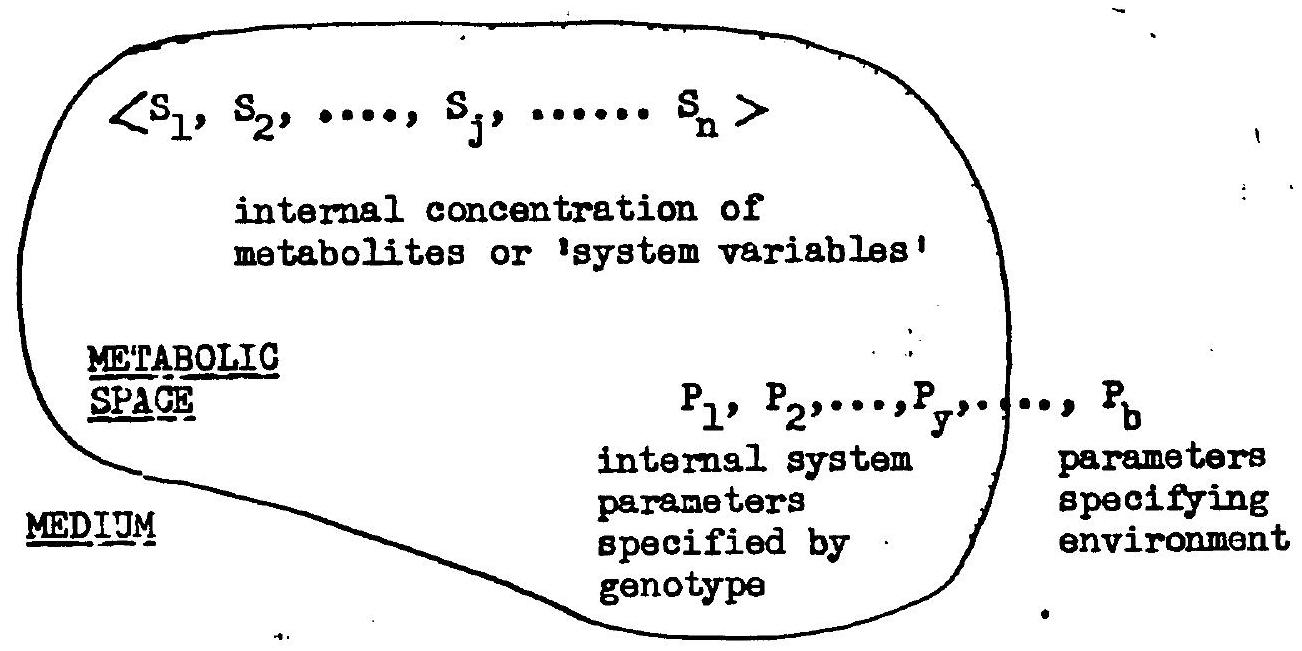
\includegraphics[scale=0.26]{2023_01_30_a974a42f7b7381f3f940g-025}}

The surrounding space is assumed to be sufficiently large and well mixed that concentrations of metabolites in it can be considered as constants in the `environment' of the metabolising volume. Since perfect mixing is also assumed internally the state of the system will be specified at any moment by the instantaneous molar concentrations $\left(S_{1}, \ldots S_{n}\right)$ ) of the $n$ variable metabolites. These, together with the fixed parameters $\left(P_{1}, \ldots P_{b}\right)$, determine the change which will ensue in the system at the next moment. This situation is expressed mathematically by saying that the `equations of motion' for the system are the set of $n$ 1st ordinary differential equations (D.E.).
%
\begin{equation}
\frac{d\left(S_{i}\right)}{d t} = \dot{S}_{i}=\varphi_{i}\left(S_{1}, \ldots \ldots, S_{n}, P_{1}, \ldots \ldots, P_{b}\right)
\label{eqn:11}
\end{equation}
%
The parameters $P$ include the constant concentration of environmental metabolites, kinetic constants belonging to genetically defined proteins, and other determinants such as the volume and surface area of the metabolising space. For the present the precise nature of the nonlinear functions $\varphi_{i}(\ldots$) may be left open, although it is clear that they will depend on expressions giving the instantaneous rates of the various metabolic transformation both within the system and across its surface. The respective contributions of genotype and environment to the properties of an organism are thus represented in the abstract problem as the way in which the solution of \eqref{eqn:11} depends on $P_{1}, P_{2}, \cdots, P_{b}$.

`Long term' means that interest is primarily in the solution of \eqref{eqn:11} a long time after its release from initial conditions $S_{i}^{0}$. Such a solution may approach a stationary steady state, when a set of values $S_i$ arise such that all the $\dot{S_i}$ become zero, or alternatively, a steady-state, in with the $S_{i}$ arise such that $S_{i}$ do not become time independent but a trajectory arises such that the system repeats its motion at regular intervals, $T$, satisfying the conditions
%
$$ \int_\alpha^{\alpha + T} \dot{S}_i dt = 0 $$
%
where $\alpha$ is an arbitrary large time. Such steady state trajectories are clearly completely characterised if the values of the $S_{i}$ are known at just one point on the trajectory. A third possible long term solution is one which is neither stationary nor steady state.

It seems clear, in the context of this discussion, that attention should be concentrated on the long term solutions \eqref{eqn:11}. Such solutions do not depend precisely on arbitrary initial conditions, but only on the system's genetically specified set of proteins together with the concentration of chemicals external to the system. If there are alternative solutions the $S_{i}^{0}$ will determine which one is reached. In principle the way is now clear to study the dependence of the long term solutions of \eqref{eqn:11} on the parameters $P_{1}, P_{2}, \ldots$, such dependence being representative of the more general dependence of the phenotype on the genotype and the environment for real genetic systems (organisms).

\section{Evaluating the stationary state}

In practice, however, even such abstract studies cannot be carried out by mathematical manipulation of \eqref{eqn:11} but, owing to the large number of system variables $S_{i}$ and the non-linearity of the functions $\varphi_{i}(\hspace{2pt})$, must be done numerically with the aid of a computer only on the simplest assumptions, namely that all $\varphi_{i}(\hspace{2pt})$ are linear functions of the $S_{i}$, can an explicit algebraic stationary steady state solution of \eqref{eqn:11} be obtained and such linear models, whilst of considerable interest, do not properly allow for basic aspects of metabolic organisation like bimolecularity and feedback inhibition.

With regard to obtaining the long term solution of \eqref{eqn:11} by numerical means and for specific values of the parameters $P_{1}, P_{2} \ldots$, there are two distinct situations, that in which the solution is a stationary one, and that where it is a non-stationary steady state or limit cycle. In both cases our interest lies not only in the solution but also in the response or sensitivity of this solution to the parameters P, that is in the influence of variation of genotype and environment on the phenotype. This response will appear naturally in the form of a matrix since it is the response of the phenotype, represented by a group of measurements on the system, to the genotype represented by a group of system parameters.

For the case of a system possessing a stationary solution the equations to be solved are, from \eqref{eqn:11}, the $n$ non-linear simultaneous equations
%
\begin{equation}
\varphi_{i}\left(S_{1}, S_{2}, \ldots, P_{1}, P_{2}, \ldots \right)=0
\label{eqn:12}
\end{equation}
%
Suppose we possess a concentration vector $S_{i}$ such that each equation differs from zero by only a small deviation $d_{i}$ then
%
\begin{equation}
d_{i} = \varphi_{i}\left(S_{1}, S_{2} \ldots\right)
\label{eqn:13}
\end{equation}
%
The problem of finding the stationary solution $\olsi{S}_{i}$ is that of how to adjust the $S_{i}$ in \eqref{eqn:13} so that all $d_{i}$ approach zero.

Let $\delta S_{i}$ be the necessary adjustment to $S_{i}$ so that $\olsi{S}_{i} = S_{i} + \delta S_{i}$. Now, since $\olsi{S}_{i}$ is the exact solution, $\varphi_{i}\left(\olsi{S}_{1}, \olsi{S}_{2}, \ldots\right.)=0$

or
%
$$
\varphi_{i}\left(S_{1} + \delta S_{1}, S_{2} + \delta {S_{2}}, \ldots \right) = 0
$$
%
which, ignoring terms above 1st degree in a Taylor expansion, gives
%
$$
\varphi_{1}\left(S_{1}, S_{2}, \ldots\right) + \sum_{j=1,n} \frac{\partial \varphi_{i}}{\partial S_{j}} \times \delta S_{j}=0
$$
%
In vector and matrix notation and using (1.3) this becomes
%
\begin{equation}
d_{i} \bumpeq \left[\frac{\partial d_{i}}{\partial S_{j}}\right] \cdot \delta S_{j}
\label{eqn:14}
\end{equation}
%
An approximate $\delta S_{i}$ is thus given by solving \eqref{eqn:14}
%
\begin{equation}
\delta S_{j} = -\left[\frac{\partial d_{i}}{\partial S_{j}}\right]^{-1} \cdot d_{i}
\label{eqn:15}
\end{equation}
%
The numerical solution of \eqref{eqn:12} then consists in progressively correcting the existing $S_{1}$ using \eqref{eqn:13} and \eqref{eqn:15} until the deviations $d_{i}$ are sufficiently close to zero. This `iterative' process will be returned to in CH. IV when the numerical and computer aspects will be discussed.

The matrix $\left[\frac{\partial d_{i}}{\partial S_{j}}\right]$ or $\left[\frac{\partial \varphi_{i}}{\partial S_{j}}\right]$, evaluated at the stationary solution, is also involved in finding the sensitivity of this solution to small changes in $P_{1}, P_{2}$, etc. In this case if the original solution was $\olsi{S}_{i}$ the new solution, $\olsi{S}_{i} + \delta \olsi{S}_{i}$ is one corresponding to, say, the change $P_{1} \rightarrow P_{1} + \delta P_{1}$, and we have the stationary condition \eqref{eqn:12} to satisfy for both the old and the new solution.
%
$$ \mbox{Thus } \psi_{i}\left(\olsi{S}_{1}, \olsi{S}_{2}, \ldots, P_{1}, P_{2}, P_{3} \ldots\right)=0, \text { for } 1=1 \text { to } N $$
\vspace{-6pt}
$$ \mbox{and also } \psi_{i}\left(\olsi{S}_{1}+\delta \olsi{S}_{1}, \olsi{S}_{2}+\delta \olsi{S}_{2}, \ldots P_{1}+\delta P_{1}, P_{2}, P_{3}\right)=0, \text { for } i=1 \text{ to } N $$
%
\vspace{14pt}
Using these two conditions and assuming $\delta \mathrm{P}_{1}$ sufficiently small for higher terms in the Taylor expansion to be ignored we get
%
$$ \frac{\partial \varphi_{i}}{\partial P_{1}} \cdot \delta P_{1} + \sum \frac{\partial \varphi_{i}}{\partial S_{j}} \cdot \delta \olsi{S}_{j}=0 $$
%
\begin{equation}
\frac{\delta \olsi{S}_{i}}{\delta P_{1}} = -\left[\frac{\partial \varphi_{i}}{\partial S_{j}}\right]^{-1} \cdot \frac{\partial \varphi_{i}}{\partial P_{1}}
\label{eqn:16}
\end{equation}

%
The relation \eqref{eqn:16} shows how stationary values of the system variables $\olsi{S}_{i}$ will respond to a small change in a parameter and can be used as a basis for considering how a general phenotype `measure' made on a stationary system will respond. Such a measure, which reflects one aspect of the phenotype, is conceived as being the result, $\olsi{M}$, of a particular measuring operation carried out upon the stationary system. $\olsi{M}$ will depend upon the variables defining the stationary state and possibly some system parameters so that in general
%
\begin{equation}
\overline{M}=\olsi{M}\left(\olsi{S}_{1}, \ldots \olsi{S}_{n}, P_{1}, \ldots P_{b}\right)
\label{eqn:17}
\end{equation}
%
Here the notation $\olsi{\mathrm{M}}(\ldots)$ merely spans, the ``function of certain arguments, whose value is $\olsi{M}$''. The response of $\olsi{M}$ to a particular parameter, say $P_{1}$, is conveniently defined as the `sensitivity coefficient' $C_{P_{1}}^{\olsi{M}}$ which compares the fractional response in $\olsi{M}$ to the small fractional disturbance in $P_{1}$ which produced it. This concept is developed further in CH. III but for the moment we can write
%
$$ C^{\olsi{M}}_{P_1} = \frac{P_1}{\olsi{M}} \frac{\partial \olsi{M}}{\partial P_1} $$
%
Using \eqref{eqn:16} and \eqref{eqn:17} we therefore get
%
\begin{equation}
\mathrm{C}_{P_1}^{\olsi{M}} = \frac{1}{\olsi{M}} \frac{\partial M}{\partial \olsi{S}_{j}} \times\left[\frac{\partial \varphi_{i}}{\partial S_{j}}\right]^{-1} \times P_{1} \frac{\partial \varphi_{i}}{\partial P_{1}}
\label{eqn:18}
\end{equation}
%
More generally the phenotype is described by a group of such measures $\olsi{M}_{1}, \ldots, \olsi{M}_{x}, \ldots \olsi{M}_{a}$ and the genotype and environment by a group of system parameters subject to variation $P_{1}, \ldots, P_{y}, \ldots, P_{b}$. The sensitivity of the phenotype to the genotype and the environment will then be displayed in the matrix of coefficients $\left[C_{P_{y}}^{\olsi{M_{X}}}\right]$, where
%
\begin{equation}
\left[C_{P_{y}}^{\olsi{M}_{X}} \right]=\left[\frac{1}{\olsi{M}_{X}} \frac{\partial \olsi{M}_{X}}{\partial \olsi{S}_{j}}\right] \times\left[\frac{\partial \varphi_{i}}{\partial S_{j}}\right]^{-1}  \times\left[P_{y} \frac{\partial \varphi_{j}}{\partial P_{y}}\right]
\label{eqn:19}
\end{equation}
%
The matrix $\left[\frac{\partial \varphi_{i}}{\partial S_{j}}\right]$ which appears in \eqref{eqn:17} and \eqref{eqn:19} is in fact also the matrix which underlies the dynamical behaviour of the system when close to the stationary state.

Thus suppose the system to be close to a stationary state so that $S_{i}=\olsi{S}_{i} + X_{i}$ where $X_{i}$ is small. Inserting this in \eqref{eqn:11} and ignoring terms above 1st order in the expansion we get
%
\begin{equation}
\dot{X}_{j} = \left[\frac{\partial \varphi_{i}}{\partial S_{j}}\right]_{S_{j}=\olsi{S}_{j}} \times X_{j}
\label{eqn:110}
\end{equation}
%
thus the `dynamical matrix', $D$, of the system is just $\left[\frac{\partial \varphi_{i}}{\partial S_{j}}\right]_{S_{j}=\olsi{S}_{j}}$.

The stability or otherwise of the stationary solution will then depend on whether the `eigenvalues' of $D$ all have negative real parts.

\section{The limit cycle}

Can similar techniques be used when a system does not possess a stationary steady state? Let us consider a system possessing a limit cycle type of `long term' solution, when it may be possible to use such a technique. Suppose that we have a trajectory close to an exact solution and defined by a concentration vector $S_{i}$ and period $T$ then the deviations defined by
%
\begin{equation}
d_{i}=\int_{t}^{t+T} \varphi_{1}\left(S_{1}, S_{2}, \cdots \cdot\right) \cdot dt
\label{eqn:111}
\end{equation}
%
correspond to the deviations of \eqref{eqn:13} in the stationary case. The integration referred to in  \eqref{eqn:111} is performed on the set of D.E. \eqref{eqn:11}, starting at time $t$ with the proposed vector $S_{i}$. The meaning of these residues is illustrated below.

\begin{center}
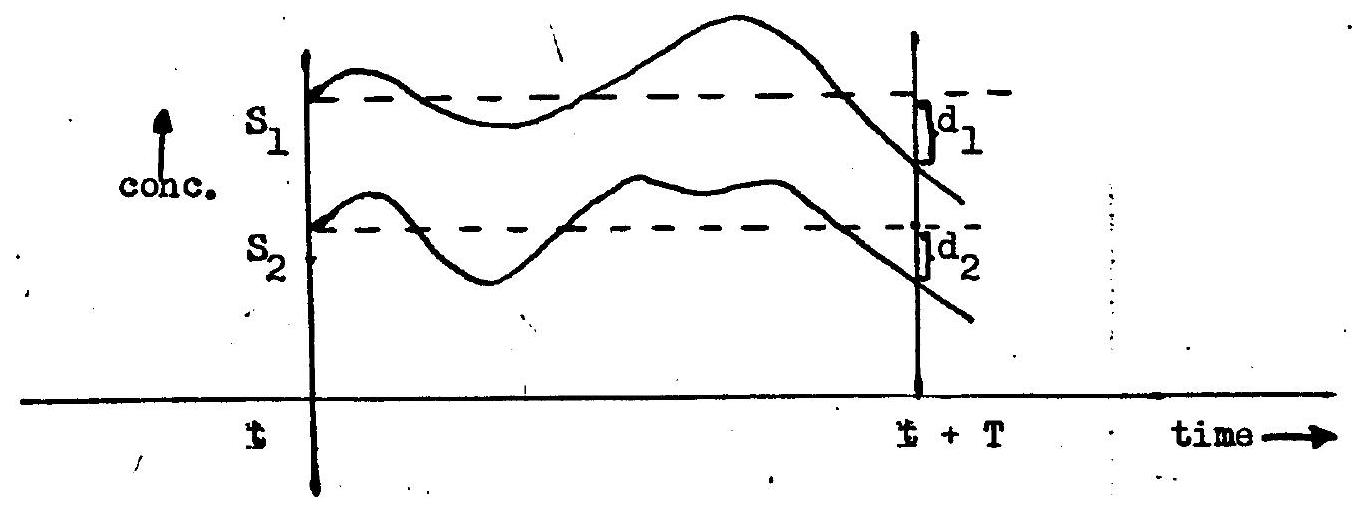
\includegraphics[max width=\textwidth]{2023_01_30_a974a42f7b7381f3f940g-033}
\end{center}

The problem of finding an exact solution is, as before, to manipulate the approximate solution until the $d_{i}$ are sufficiently close to zero. This can be done by adjusting all but one of the $S_{i}$ and also the approximate period $T$, parameters which can be designated $\xi_1$ to $\xi_n$. The holding constant of one of the $S_{i}$ merely serves to define the arbitrary time, $t$, which is being used to characterise the final limit cycle. The small corrections to be applied to the existing values of the parameters are calculated by the relation
%
\begin{equation}
\delta \xi_{j} = -d_{i} \bigg/\left[\frac{\partial d_{i}}{\partial \xi_{j}}\right]
\label{eqn:112}
\end{equation}
%
which is analogous to relation \eqref{eqn:15}, and a similar `iteration' is performed using \eqref{eqn:112} and  \eqref{eqn:111}. The matrix $\left[\frac{\partial d_{i}}{\partial \xi_{j}}\right]$ can, as before, also be used to discover the sensitivity of measures connected with the limit cycle to the parameters $P_1, P_2, \cdots P_b$.

There is, however, an important practical difference between the two cases just discussed in that the evaluation of the $d_i$ for the limit cycle case involves, even on the best assumptions, many hundreds of times more computer operations than does the stationary case. This is because the integration of the system of D.E. \eqref{eqn:11} over the period $T$ involves many hundreds of evaluations of the $S_i$, each of which corresponds to one $d_i$ evaluation in the stationary state computation.

If the period $T$ is large or the equations difficult to integrate the factor may be even worse and the difficulty is further compounded by the requirement that the $d_i$ have to be calculated to a high accuracy if the numerical differentiation involved in estimating the matrix $\left[\frac{\partial d_i}{\partial \xi_j}\right]$ of \eqref{eqn:112} is to be reliable. It appears, therefore, that whilst the stationary type of computation proves quite feasible for reasonably large networks, say less than forty enzymes, it becomes totally impracticable for networks having limit cycle solutions. This conclusion applies a fortiori to systems whose `long term' solution, although regular in some sense, cannot be described by limit cycles. In these circumstances, remembering that an interact in gene action involves networks of some size and complexity, consideration can only be given to systems possessing stable stationary state solutions. This limitation seems unavoidable, whether it turns out to be serious will depend on how frequently non stationary long term behaviour is encountered in metabolic systems under study.

\section{The use of rate equations}

Accepting then the considerable simplification that only stationary solutions of homogeneous multi-enzyme systems will be considered it is hoped that such solutions will still represent important. aspects of the genotype-phenotype relation. This hope rests mainly on the strategy that minimal compromise will subsequently be made in representing the structure of metabolic networks, the structure clearly being critical to any attempt at representing gene-action.

The nature of the system variables $S_{i}$ has deliberately been left open until this point. A reasonably complete set of such variables for a metabolic system has usually been taken as a set of concentrations of intermediary metabolites together with a set of concentrations of enzymic intermediates. The set of dynamical functions $\varphi$ (..) are then written down, using the `Guldberg-Waage' law of mass-action, and used as a basis for further analysis, as for example in Pring (1967).

However, when interest is centred, as here, on the properties of the stationary state it is possible to avoid considering enzymic intermediates by using the fact that when the complete system is at a stationary state so will be the enzymic intermediates belonging to each enzyme. The `net flux' carried by each enzyme at the stationary state will then be given by the King-Altman rate expression of steady state enzyme kinetics as discussed in the introduction. Thus the number of system variables is reduced to the number of intermediary metabolites and expressions $\varphi_{i}(\ldots)$ for their rates of change become sums and differences of rate expressions. The expressions $\varphi_{i}$ (\ldots) made up

\bigskip
\centerline{\bf\large General theoretical aspects of multi-enzyme systems}

\begin{center}
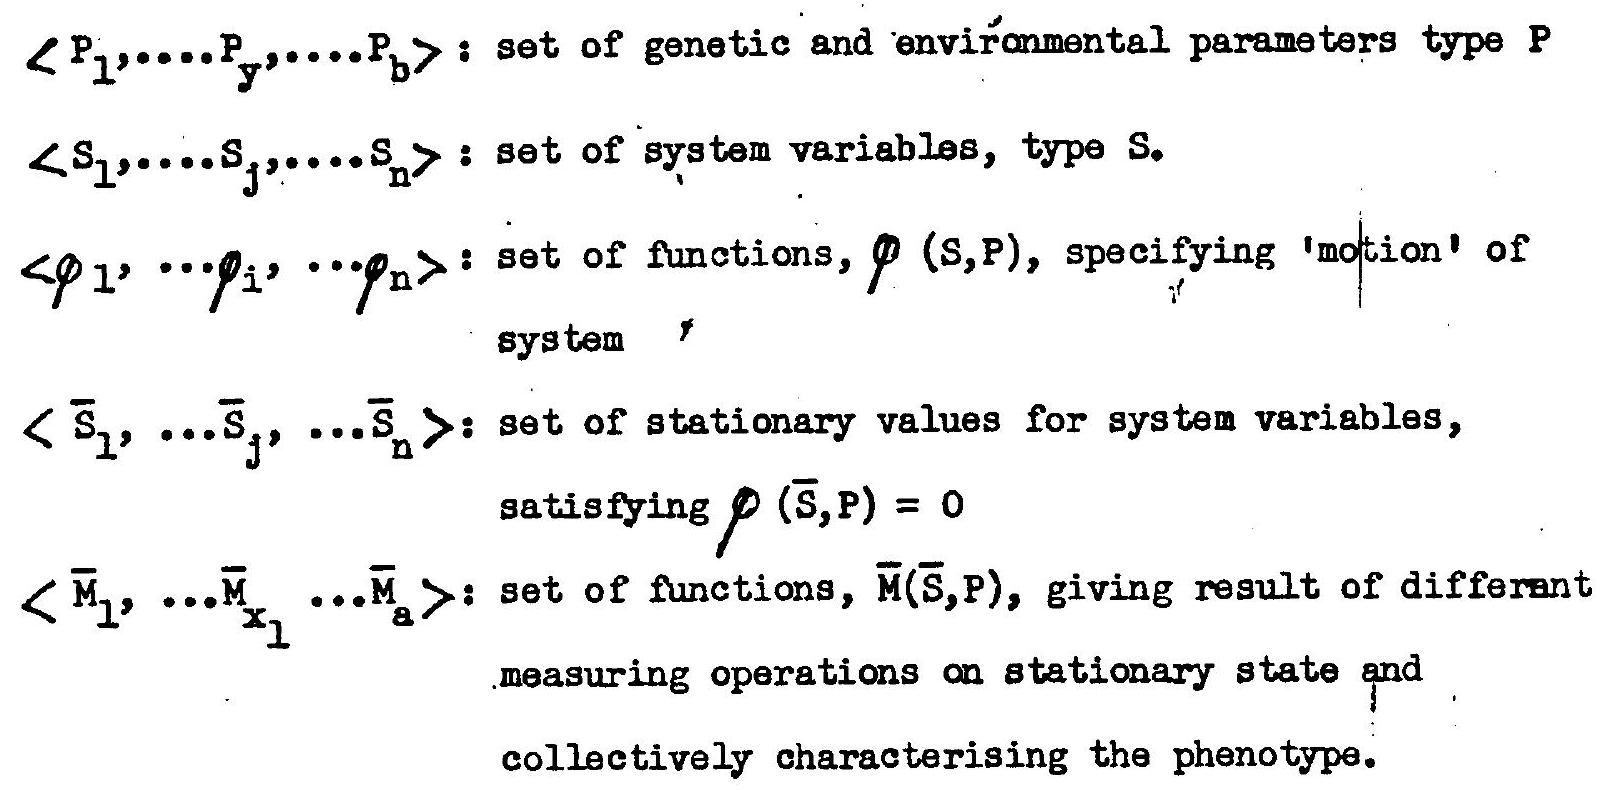
\includegraphics[max width=\textwidth]{2023_01_30_a974a42f7b7381f3f940g-036}
\end{center}

\pagebreak
\centerline{\bf\large Numerical operations}

i) Evaluate matrix $\left[D'\right]=\left[\frac{\partial \varphi_{i}}{\partial S_{j}}\right]$ at present values of $S_{j}$ by numerical approximation.

ii) Use it to find $\olsi{S}$ by means of the `iteration'

$$
\begin{aligned}
\mbox{1: } & \delta S_{j} = \left[D^{\prime}\right]^{-1} \cdot \varphi_{i} \\
& S_{j} \leftarrow S_{j} + \delta S_{j} \\
& \rightarrow \mbox{(goto) } 1 \text { unless all } \varphi_{i} \bumpeq 0
\end{aligned}
$$

Having thus obtained $\olsi{S}$ and $D=\left[\frac{\partial \varphi_{i}}{\partial {S_{j}}}_{\mbox{at }S=\olsi{S}}\right]$

iii) Compute the phenotype/genotype, environment) sensitivity matrix using the relation

$$
\left[
C_{P_y}^{\olsi{M}_X}\right] = \left[\frac{1}{M_X} \frac{\partial M_X}{\partial S_j}\right] \times [D]^{-1} \times\left[\frac{P_y \partial \varphi_i}{\partial P_y}\right]
$$

iv) Characterise the dynamics of the system close to the stationary state by extracting eigenvalues of $\left[ D \right]$.

\noindent\rule{\textwidth}{1pt}

in this way will only approximate to the `true' dynamics of the system, but Pring (1967) has shown that this approximation may be a very good one. However, the stationary state and its properties will not be in any way affected by this simplification and the dimension of a given system will be reduced by a considerable factor. For example a system with 20 metabolites and 25 enzymes each requiring, on the average, 4 enzymic intermediates to describe its kinetics, would have a dimension of 120 system variables. In this case a reduction in dimension of 6 fold would result from the use of rate expressions in making up the functions $\varphi_{i}$ for the 20 intermediate metabolites, properties of the stationary state would be identical with the `true' system and even the dynamics would be a good approximation.

Accordingly, unless otherwise stated, system variables will be taken to be the set of intermediary metabolite concentration. The set of dynamical functions $\varphi_{i}$ attached to them will then be an approximation to the true dynamics, involving the use of rate expressions, which nevertheless leaves the properties of the stationary state unaltered.

Our general theoretical and computational framework for multienzyme systems which possess a stationary solution is now clear. This is summarised on p.14 opposite, where it can be seen that the set of dynamical functions $\varphi_{1}, \ldots ., \varphi_{\mathrm{n}}$ and the matrix $[\mathrm{D}]=\left[\frac{\partial \varphi_{i}}{\partial S_{j}}\right]$ play an important role. The remainder of this chapter will consider the particular situation when the $\varphi_{1}$ represent systems of unimolecular reactions. Chapter II will then be concerned with progressively showing how more general systems, having the necessary realistic detail, may be formulated in terms of suitable sets of functions $\varphi_{i}$, themselves based on rate expressions.

The remainder of this chapter will consider the particular situation when the $\varphi_1$ represent systems of unimolecular reactions. Chapter II will then be concerned with progressively showing how more general systems, having the necessary realistic detail, may be formulated in terms of suitable sets of functions $\varphi_i$, themselves based on rate expressions.

\section{Unimolecular systems}

These systems, often arising as a first approach to more realistic ones, are of interest because in certain cases explicit solutions for the stationary state, or \underline{S.S.} in terms of the parameters can be obtained. In addition it proves possible to consider, in a general way, whether or not the \underline{S.S.} of unimolecular systems are stable or not. Although these explicit solutions and stability properties apply strictly only to unimolecular systems they provide a useful analytic background against which numerical solution of the more general systems of CH II can be evaluated.

For the present unimolecular systems are considered to have a fixed volume, $V$, and to have enzyme quantities prescribed parametrically (genetically). Later, in CH II, these restrictions will be relaxed somewhat to include `growing systems', when $\dot{V} \neq 0$, and `enzyme regulation' in which enzyme quantity is not parametrically prescribed.

\section{The straight chain}

A start will be made with the simplest unimolecular system, that of the `straight chain of linear reactions', and this will be considered in some detail. Such a system, consisting of $n$ variable metabolites and $m(=n+1)$ linear enzymes, is represented in the following diagram as taking place in a fixed volume $V$ and converting an external metabolite, $X_1$, to another, $X_2$.

\begin{center}
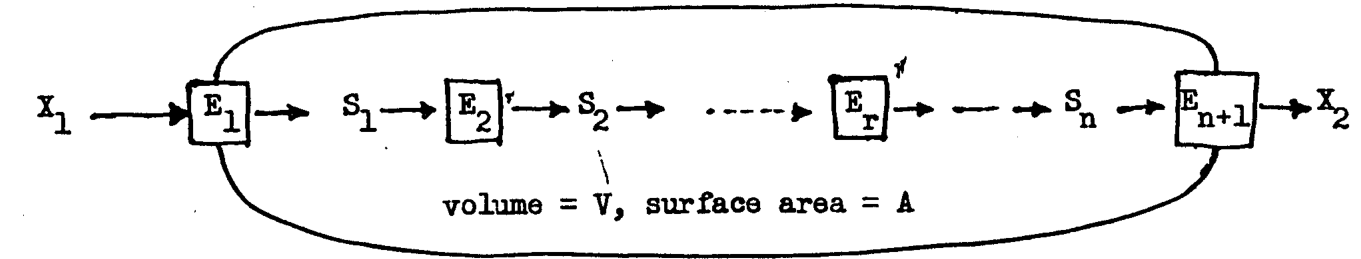
\includegraphics[max width=\textwidth]{figure1_chain}
\end{center}

By `linear' is meant that the rate-expressions for the separate reactions of type, $A \rightleftarrows B$, are of the form.
%
\begin{equation}
f = \rho(A-B / K) \tag{1.13a}
\label{eqn:113a}
\end{equation}
%
where $f$ is the net flux from A to $B$ per unit quantity of enzyme, $K$ is the equilibrium constant for the reaction and $\rho$ is a kinetic constant. In fact every enzyme catalyzed reaction will have a non-linear rate expression, since saturation can always occur and (1.13a) is merely an approximation which holds provided the concentrations, $A$ and $B$, remain within certain limits. For example the simple non linear rate-expression for a unimolecular reaction mentioned in the introduction was of the form
%
\begin{equation}
f = \frac{\vecur{T}}{\vecur{M}}\left(A - \frac{B}{K}\right) /\left(1 + \frac{A}{\vecur{M}} + \frac{B}{\vecul{M}}\right) \tag{1.13b}
\label{eqn:113b}
\end{equation}
%

This approximates to the linear form (1.13a) provided $A \ll \vecur{M}$ and $B \ll \vecul{M}$, the constant $\rho$ then equals $\frac{\vecur{T}}{\vecur{M}}$.

In the diagram $E_{1}, E_{2}, \ldots$ are used both as `names' for the enzymes and also to refer to their concentrations, similarly for the metabolites $S_{1}, S_{2}, \ldots$. Provided that the metabolites are well mixed the enzymes can be distributed non uniformly in the volume in which case $E_{r}$ refers to the average concentration. Transport enzymes such as $\mathrm{E}_{1}, \mathrm{E}_{\mathrm{n+l}}$ will have to be situated, not necessarily uniformly, on the surface but their `linear' rate expressions will be formally similar. Even if transport is non-enzymic and therefore depends on the surface area, A, there will be an effective `concentration of area', $A/V$, which will be genetically (parametrically) defined and will play a similar role to enzyme concentration.

Considering the rate of change of the 1st metabolite in the whole volume
%
$$
\frac{d\left(V_{X} S_{1}\right)}{dt} = \left(E_{1} \times V\right) \rho_{1}\left(X_{1} - \frac{S_{1}}{K_{1}}\right) - \left(E_{2} \cdot V\right) \rho_{2}\left(S_{1} - \frac{S_{2}}{K_{2}}\right)
$$
%
or
%
\begin{equation}
\dot{S}_{1} = E_{1} \rho_{1}\left(\mathrm{X}_{1}-\frac{\mathrm{S}_{1}}{\mathrm{K}_{1}}\right)-\mathrm{E}_{2} \rho_{2}\left(\mathrm{S}_{1}-\frac{\mathrm{S}_{2}}{\mathrm{K}_{2}}\right)-\left(\frac{1}{\mathrm{V}}\dot{V}\right) \mathrm{S}_{1}
\label{eqn:114}
\end{equation}
%
The products $E_{r} \rho_{r}$ etc. can be written as $v_{r}$. Where $v_{r}$ means the activity of the rth enzyme per unit volume of the system when the substrate has unit and the product zero concentration. Writing $F_{1}, F_{2}$, as, the net fluxs/unit volume of the system and remembering that $\left(\frac{1}{\olsi{V}}\dot{V}\right)$ is zero, the set of dynamical function $\varphi_{1}, \ldots, \varphi_{\mathrm{n}}$ are given by
%
\begin{equation}
\begin{aligned}
 \varphi_{1} &=\dot{S}_{1}=v_{1}\left(\mathrm{X}_{1}-\frac{\mathrm{S}_{1}}{\mathrm{K}_{1}}\right)- v_{2}\left(\mathrm{S}_{1}-\frac{\mathrm{S}_{2}}{\mathrm{K}_{2}}\right)=\mathrm{F}_{1}-\mathrm{F}_{2} \\[4pt]
\varphi_{2}&=\dot{\mathrm{S}}_{2}=v_{2}\left(\mathrm{S}_{1}-\frac{\mathrm{S}_{2}}{\mathrm{K}_{2}}\right)-v_{3}\left(\mathrm{S}_{2}-\frac{\mathrm{S}_{3}}{\mathrm{K}_{3}}\right)=\mathrm{F}_{2}-\mathrm{F}_{3} \\
& \vdots
\\
 \varphi_{n}&=\dot{S}_{n}=v_{n}\left(\mathrm{S}_{n-1}-\frac{\mathrm{S}_{\mathrm{n}}}{\mathrm{K}_{n}}\right)-v_{n+1}\left(\mathrm{S}_{\mathrm{n}}-\frac{\mathrm{X}_{2}}{\mathrm{K}_{n+1}}\right)=\mathrm{F}_{n}-\mathrm{F}_{n-1}
\end{aligned} \tag{1.15a}
%\label{eqn:115}
\end{equation}
%
The conditions, $\varphi_{i}=0$, for a stationary solution give rise to a set of $n$ linear simultaneous equations for the $n$ unknown stationary values $\olsi{S}_{i}$ and these equations could be solved; because of their simple structure, by straightforward algebraic elimination. However, they will be treated in a more general way both to illustrate the methods just described and to facilitate extension later to the "non-linear straight chain" where algebraic elimination is not possible.

The equations (1.15a) are equivalent to the `band matrix' equation

\begin{center}
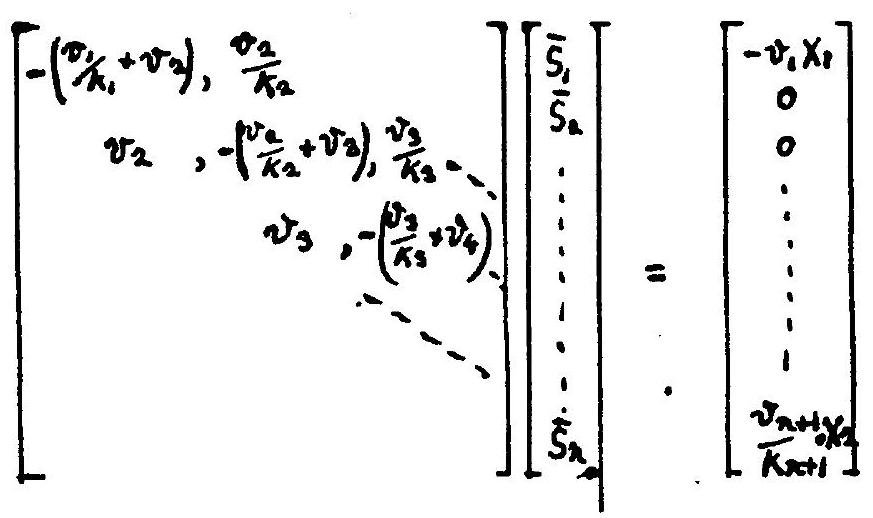
\includegraphics[scale=0.35]{2023_01_30_a974a42f7b7381f3f940g-041}  \mbox{\hspace{15pt} (1.15b)}
\end{center}
\stepcounter{equation}
\stepcounter{equation}
Hence there is just one S.S. which furthermore turns out to be completely stable in the sense that the dynamics of the approach to this S.S. is a sum of decaying exponentials, (Denbigh, Hicks and Page, 1947). This latter property arises because the dynamical matrix $[D]$, which in this case is identical to the band matrix above, possesses special features. Since these features are of a general nature they will be dealt with later. in this chapter.

However, inverting the matrix gives little insight into how the $\olsi{S}_{i}$, or indeed important measures of the system such as the pathway flux, $\olsi{F}$, depend on the parameters.. This can be shown as follows. At the S.S. all the separate fluxes are equal to the pathway flux so that:
%
\begin{equation}
\begin{aligned}
\olsi{F}=\olsi{F}_{1} &= v_{1}\left(\olsi{X}_{1}-\frac{S_{1}}{\olsi{K}_{1}}\right) \\[4pt]
\olsi{F}=\olsi{F}_{2} &= v_{2}\left(S_{1}-\frac{S_{2}}{K_{2}}\right) \\[4pt]
\olsi{F}=\olsi{F}_{n+1} &= v_{n+1}\left(S_{n}-\frac{X_{2}}{K_{n+1}}\right)
\end{aligned}
\label{eqn:116}
\end{equation}
%
If $\olsi{F}$ is the correct pathway flux there are $n+1$ linear equations to solve for only $n$ unknowns, $\olsi{S}_{1} \ldots \olsi{S}_{n}$. This means that the coefficients must be linearly dependent and implies that their $(n+1)$ determinant is zero.
%

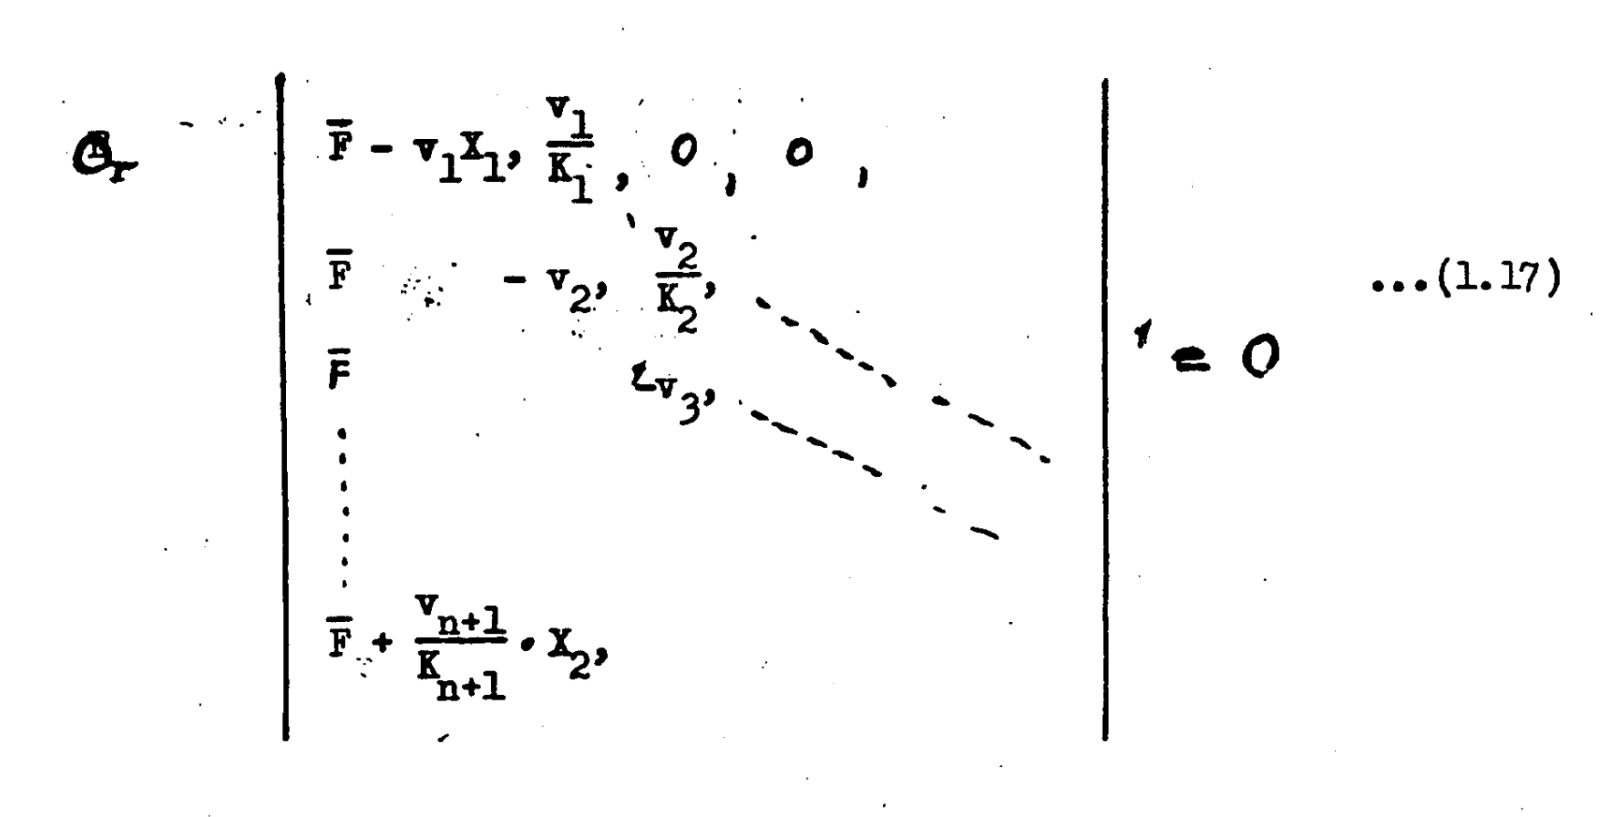
\includegraphics[scale=0.5]{figure1_17.png}

%
Since $\olsi{F}$ occurs only in the 1st column this is a simple linear equation in $\olsi{\mathrm{F}}$ and when expanded gives on simplifying this yields
%
\stepcounter{equation}

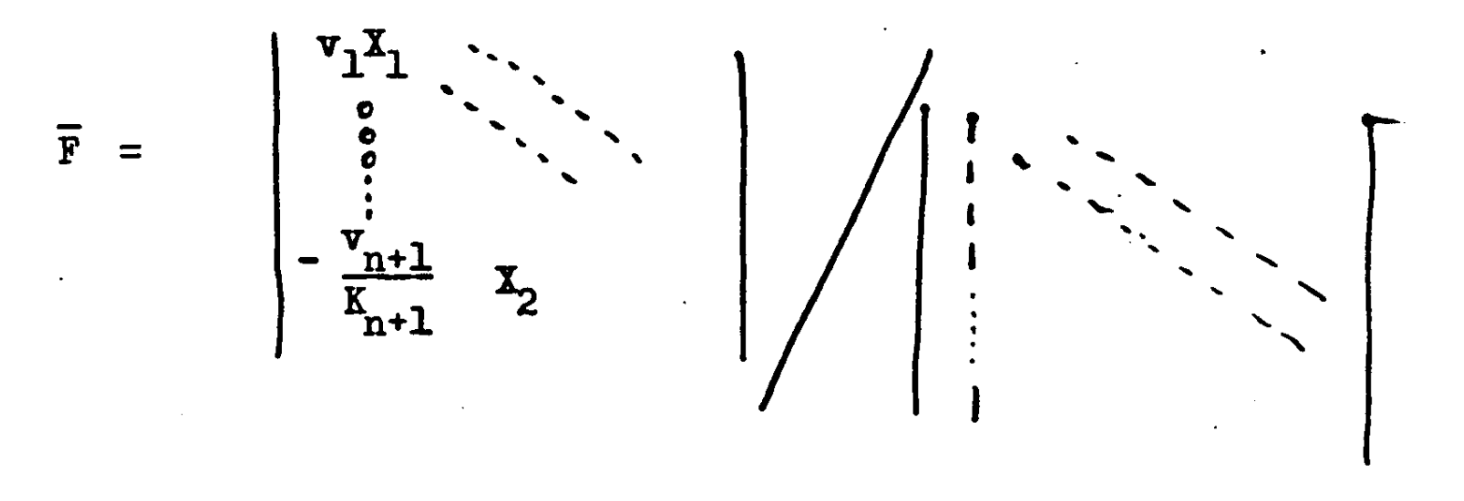
\includegraphics[scale=0.55]{figure1_17a.png}
%
%\centerline{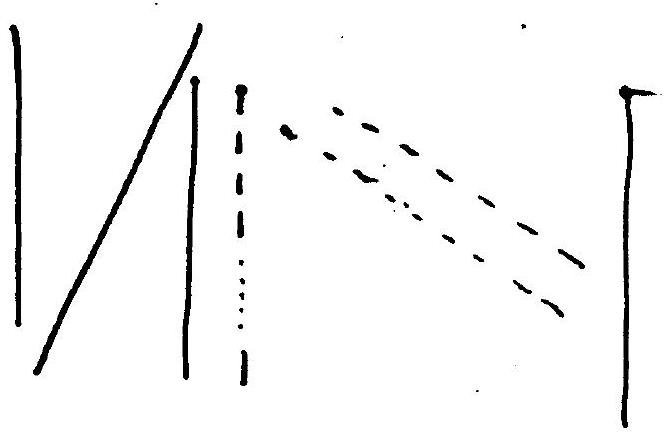
\includegraphics[scale=0.3]{2023_01_30_a974a42f7b7381f3f940g-043}}
$$
\overline{\mathrm{F}} = \mathrm{X}_1-\frac{\mathrm{X}_2}{\mathrm{K}_1 \cdot \mathrm{K}_2 \cdots \mathrm{K}_{n+1}} \bigg/
\left(\frac{1}{v_1} + \frac{1}{\mathrm{K}_1 v_2} + \frac{1}{\mathrm{K}_1 \mathrm{K}_2 v_3} +
\cdots \frac{1}{\mathrm{K}_1 \mathrm{K}_2 \cdots \mathrm{K}_n v_{n+1}}\right)  \mbox{(1.18)} $$

Having found $\olsi{F}$ it is a simple matter to compute $S_{1}, S_{2}$ etc. using successively the equations of (1.16).

\section{The sensitivity coefficient}

The relation (1.18), allows us to see explicitly exactly how the measure $\olsi{F}$ depends on the parameters $v_{1}, v_{2}, \cdots$ In this case the flux controlling effect of the separate enzymes in, the pathway will be measured by the set of sensitivity coefficients $C_{v_{i}}^{\olsi{F}}$ and an expression can be found, employing the usual definition.

Thus
%
\stepcounter{equation}
\begin{equation}
\begin{aligned}
C_{v_{i}}^{\olsi{F}} &= \frac{v_{i}}{\olsi{F}} \cdot \frac{\partial \olsi{F}}{\partial v_{i}}=v_{i} \frac{\partial \log (\olsi{F})}{\partial v_{i}} \\
&=v_{i} \left(-1 \bigg/ \frac{1}{v_{1}}+\frac{1}{K_{1} v_{2}} \cdots \cdots\right) -\frac{1}{K_{1} K_{2} \ldots v_{i}^{2}} \\
C_{v_{i}}^{\olsi{F}} &=\frac{1}{K_{1} \ldots K_{i-1} v_{i}} \bigg/\left(\frac{1}{v_{1}}+\frac{1}{K_{1} v_{2}}+\ldots \ldots\right)
\end{aligned}
\label{eqn:119}
\end{equation}

The two properties, $0 < C_{v_i}^F < 1$ and $\displaystyle \sum_{i=1..n} C_{v_i}^F = 1$ immediately follow.

Since \eqref{eqn:119} is of the form, $C^{F}_{v_{i}} = \frac{a_{i}}{\sum a_{i}}$, it is clear that the separate coefficients are all positive and less than unity and that in addition the sum of the separate coefficients is unity.

This leads to the important result that if any enzyme is found to have a control coefficient of approximately one it must be the controlling or `throttling' enzyme in the sequence since the sum of all the other control coefficients will be small. For example a system having four reactions all with $K_{E}=1$, three catalysed by enzymes of activity $v$ and one of them, say the 2nd, by an enzyme of activity $v/9$ would be expected to have rate-control mainly from the second enzyme.

Broadly how strong this effect is can be seen from substituting in \eqref{eqn:119},
%
$$
C^{\olsi{F}}_{v_2} = \frac{1}{v/9} \bigg/ \frac{1}{v} + \frac{1}{v/9} + \frac{1}{v} + \frac{1}{v} = \frac{9}{12} = 75 \%
$$
%
Thus of the total $100 \%$ control available $75 \%$ is `owned' by the 2nd enzyme and $8.3 \%$ by each of the others.

In a real situation, we may wish to know which is the limiting enzyme in a sequence but find it inconvenient or impossible to estimate the response of $\olsi{F}$ to a modulation in $v_{i}$ for several enzymes. In these circumstances it would be useful if some other `measure' were diagnostic of rate control. Such a `diagnostic' might be related to the pattern of the pools. Thus for the previous example, the pool levels are shown in the following diagram if $X_{1}$ is taken as 100 and $X_{2}$ as zero.

\begin{center}
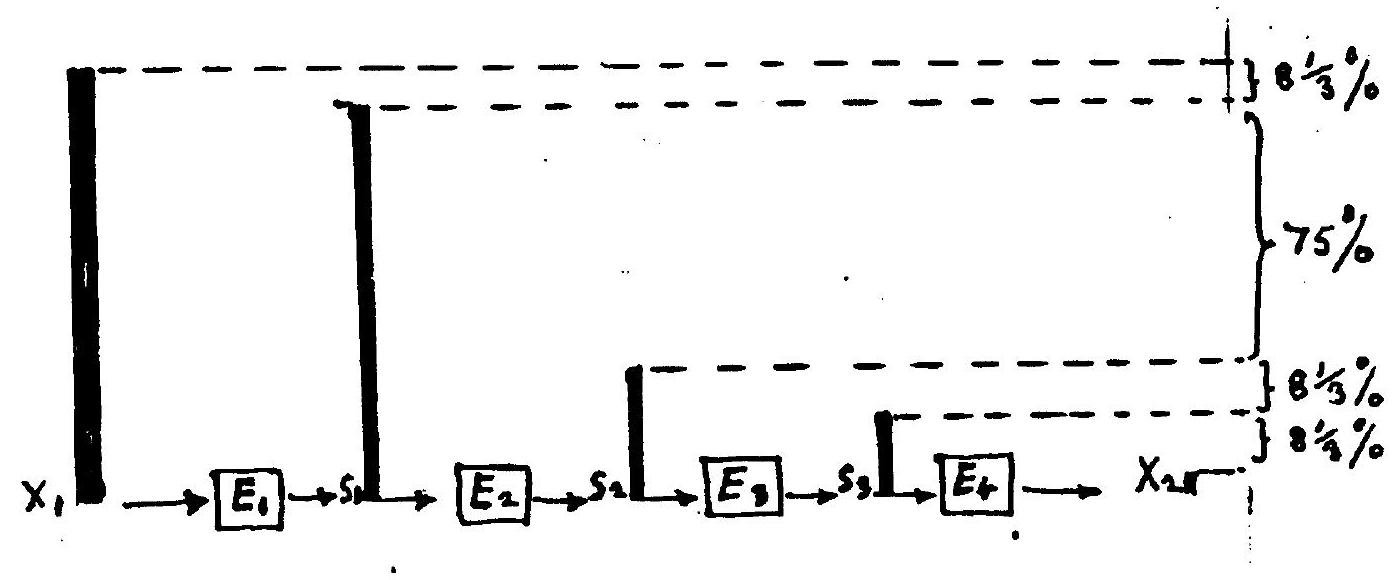
\includegraphics[max width=\textwidth]{2023_01_30_a974a42f7b7381f3f940g-045}
\end{center}

In this case the main drop is indeed across the 2nd enzyme and in fact it is true that the difference between pools on either side of an enzyme is a measure of its relative rate controlling effect. Will this be so for arbitrary $X_{1} X_{2}$ and when $K_{1} K_{2}$ etc are not unity?

From \eqref{eqn:119}
%
$$
 \quad C_{v_{i}}^{\olsi{F}} \propto \frac{1}{K_{1} K_{2} \ldots v_{i}}
$$
%
and also the set of equation \eqref{eqn:116}  can be written as
$$
\frac{1}{v_{1}} = \frac{X_{1}}{\olsi{F}} \cdot\left(\frac{X_{1}}{X_{1}}-\frac{S_{1}}{K_{1} X_{1}}\right) = \frac{X_{1}}{\olsi{F}} Q_{1}
$$

$$\frac{1}{\mathrm{K}_1 v_2} = \frac{\mathrm{X}_1}{\olsi{F}} \left(\frac{\mathrm{S}_1}{\mathrm{K}_1 \mathrm{X}_1}-\frac{\mathrm{S}_2}{\mathrm{K}_1 \mathrm{K}_2 \mathrm{X}_1}\right) = \frac{\mathrm{X}_1}{\olsi{F}}  {Q}_2$$

so that the factors $Q_{1}, Q_{2}...$ are proportional to the coefficients of the respective enzymes. The meaning of these factors is apparent when it is noted that $K_{1} X_{1}, K_{1} K_{2} X_{1}, \ldots$ are the values $, S_{1}^{*}, S_{2}^{*}$, which $S_{1}, S_{2}$ would take if the flux in the pathway were blocked and equilibrium were established along the chain. The factors $Q_{1}, Q_{2}, \ldots$ etc are then just

$$\left(1-\frac{\olsi{S}_{1}}{S_{1}^{*}}\right), \left(\frac{\olsi{S}_{1}}{S_{1}^{*}} - \frac{\olsi{S}_{2}}{S_{2}^{*}}\right), \ldots \mbox{etc.} $$

In principle then an experiment could be done which first observed the levels of $\olsi{S}_{1}, \olsi{S}_{2}$ etc. then observed the values $S_{1}^{*}, S_{2}^{*}$, which resulted from blocking the pathway. Scaling the $\olsi{S}_{i}$ by their own equilibrium values, $S_{i}^{*}$, would result in a set of numbers, the difference between successive pairs yielding $Q_{1}, Q_{2} \cdots$. One advantage of such a diagnostic would be that it only involves ratios of concentrations of single pools and hence does not depend on the metabolites being uniformly extractable.

\section{The network}

The system just dealt with at some length had a number of relatively simple properties. Thus it was completely stable, possessed only one stationary state, the sum of rate control over the enzymes was unity and finally the pool pattern gave a simple `diagnostic' of which step was exerting control. In addition there was a simple expression for the pathway flux as a function of the parameters. It will be of interest to see to what extent these properties are retained as more realistic features are introduced into unimolecular systems. Thus we fan consider a more general \underline{network} of such linear unimolecular reactions, or consider the case where saturation effects are incorporated into the rate expressions.

The general network of linear unimolecular reactions allows for more than two external metabolites and also for any amount of branching and convergence of pathways. A typical network containing nine enzymes is shown below and exemplifies the possible features.
%
\begin{center}
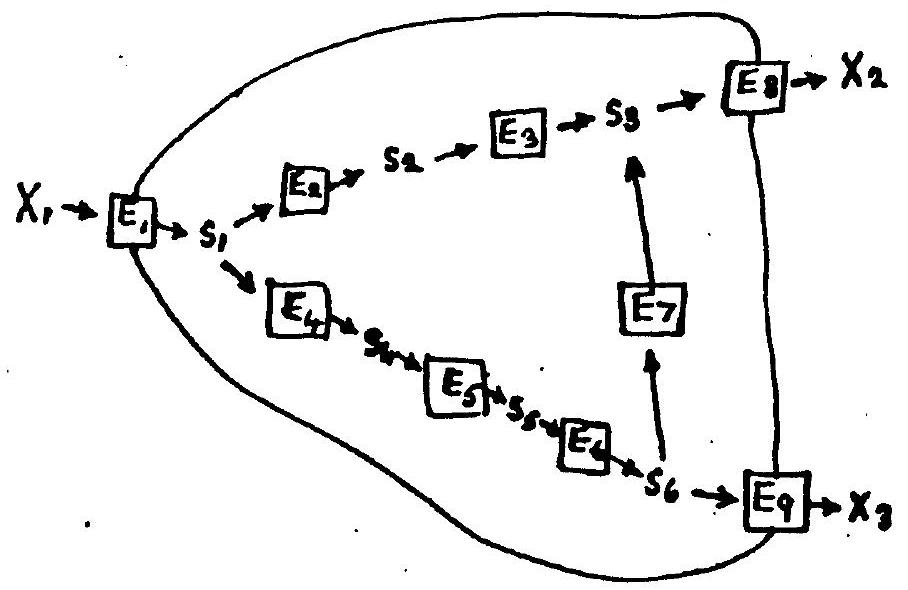
\includegraphics[scale=0.3]{2023_01_30_a974a42f7b7381f3f940g-047}
\end{center}
%
Of particular interest is that it is now possible to have a cycle of reactions in the sense that molecules leaving $S_{1}$, along one path may return on another.

The general network is allowed for in the scheme below which shows the exchange between any two arbitrary internal metabolites $S_i, S_j$ and also between any internal metabolite $S_1$ and external $X_q$. The net flux, used previously, is here considered as being made up of the +ve and -ve parts of the linear rate expression (1.13a).

\begin{center}
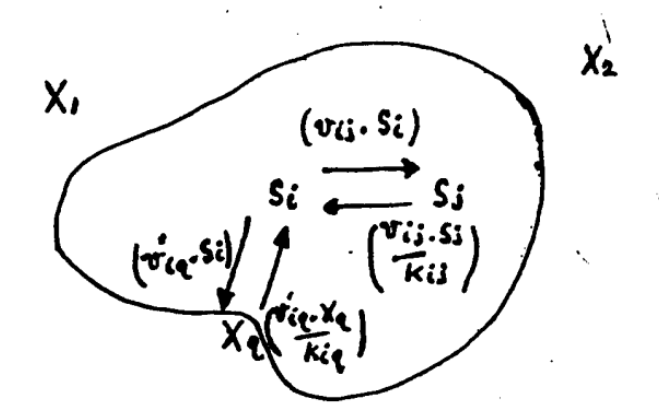
\includegraphics[scale=0.7]{figure1_system.png}
\end{center}

The constant $K_{i, j}$ is the equilibrium constant for the reaction $S_i \rightleftharpoons S_j$ and is defined as $\left(\frac{S_j}{S_i}\right)$ eq. If all the reactions are truly unimolecular then, when more than one route exists between two metabolites, the product of the $\mathrm{K}_{\mathrm{E}}$s must be the same for both routes (Levis, 1925). For example in the nine enzyme network above $\mathrm{K}_{1,2} \cdot \mathrm{K}_{2,3}=\mathrm{K}_{1,4} \cdot \mathrm{K}_{4,5} \cdot \mathrm{K}_{5,6} \cdot$ K$_{6,3}$. The dynamical equations for the general network are written down in a similar way to those for the straight chain and are

\begin{equation}
\varphi_i=\dot{S}_i=-\sum_{\mbox{all} j\neq i} v_{ij} \left(S_i-\frac{S_j}{K_{i,j}}\right)-\sum_q v_{iq}^{\prime}\left(S_i-\frac{X_q}{K_{iq}^{\prime}}\right)
\label{eqn:120}
\end{equation}

Since the network is truly unimolecular there will be a unique product of equilibrium constants between $\mathrm{X}_1$ (say) and any other metabolite, $S_i$ or $X_{q}$ Let these products be denoted by $\eta_i$ and $\eta^{\prime}_q$.

\section{The electrical analogue}

It will now be shown that if each $S_{1}$ and $X_{q}$ is scaled by its appropriate $\eta$ the equations (1.20) will assume a particularly simple form from which certain observations follow. These scaled variables are $\theta_{i}=\frac{S_{i}}{\eta_{i}}$ and $\theta_{q}^{\prime}=\frac{X_{q}}{\eta^{\prime}_q}$ and the equations (1.20) may be grouped as follows:
%
$$
\eta_{i} \times \left(\frac{\dot{S}_{i}}{\eta_{i}}\right) = -\sum v_{ij} \cdot \eta_{i}\left(\frac{S_{i}}{\eta_{i}}-\frac{S_{i}}{K_{i,j} \eta_{i}}\right)- \sum \cdots
$$
%
then noting that, by definition, $X_{i,j} \eta_{i}=\eta_{j}$ we have
%
$$
\eta_{i} \dot{\theta}_{i}=-\sum \eta_{i} v_{ij}\left(\theta_{i}-\theta_{j}\right)- \sum \eta_{i}^{\prime} v_{iq}^{\prime}\left(\theta_{i}-\theta_{q}^{\prime}\right)
$$
%
finally, introducing $\rho_{ij}=\eta_{i} v_{ij}$ and noting that this quantity is symmetric, since
%
$$
\rho_{ij}=\eta_{i} v_{ij}=\eta_{i} K_{ij} \cdot \frac{v_{i j}}{K_{i j}}=\eta_{j} \cdot v_{ji}=\rho_{ji}
$$
%
The equations (1.20) assume the form
%
\begin{equation}
\eta_{i} \dot{\theta}_{i}=-\sum_{j \neq i} \rho_{i j}\left(\theta_{i}-\theta_{j}\right)-\sum_{q} \rho_{iq}^{'}\left(\theta_{i} - \theta_{q}^{i}\right)
\label{eqn:121}
\end{equation}
%
A set of interconnected earthed capacitors will be described by exactly the same set of.equations when some of the capacitor is are connected via conductances $\rho_{i q}^{\prime}$ to fixed voltages, $\theta_{q}^{\prime}$, the ith capacitor having capacitance $\eta_{i}$ and the conductance between the ith and $j$th capacitor being $\rho_{i j}$ Thus the general enzyme network shown previously is, in this sense, exactly equivalent to the general electric network following.

\begin{center}
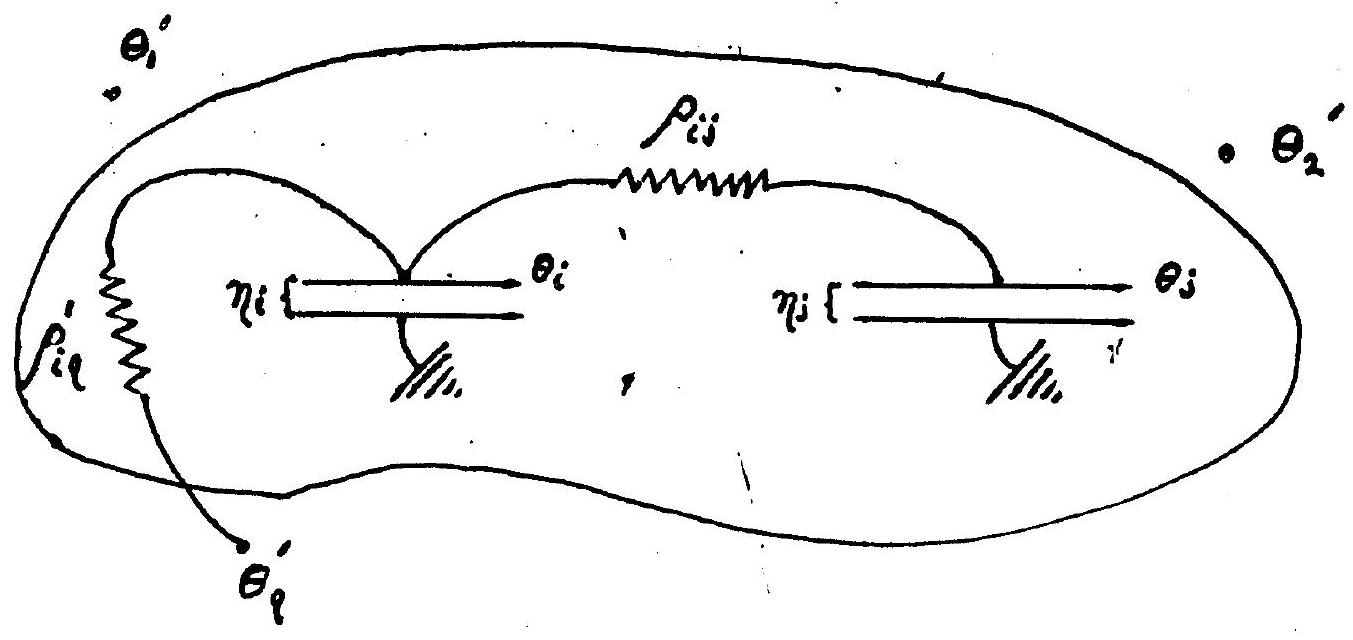
\includegraphics[max width=\textwidth]{2023_01_30_a974a42f7b7381f3f940g-050}
\end{center}

The rule of equivalence is that at the ith node of the chemical network should be placed a capacitor whose value, $\eta_{i}$, is the product of the equilibrium constants between $X_{1}$ and the node, and that each enzyme having activity $v_{ij}$ radiating from this node should be placed by a conductance of value $\eta_{i} v_{ij}$ Then the fluxes in the enzyme network will be numerically identical with the currents in the electrical system, and the voltages $\theta_{i}$ at the nodes will be related to the metabolic pools by $S_{i}=\eta_{i} \cdot \theta_{i}$. There is no confusion about the values to be given conductances, according to which node they are calculated from, since $\eta_{i} v_{ij}=\eta_{j} v_{ji}$. When interest is centred on the stationary state the values assigned to the capacitors are unimportant and the equivalent system is merely the network of conductances.

This equivalence principle makes clear why the straight chain of reactions had simple properties, since no matter how many conductances are placed in series they still behave as one conductance which can be found by a simple rule for compounding them. For more complicated networks the stationary fluxes can easily be found by applying the known Kirchoff laws.

As an example the general branched pathway will be considered. To start with consider a system with only three reactions and where $\mathrm{X}_{1}$ is converted via a branching system into $\mathrm{X}_{2}$ and $\mathrm{X}_{3}$. The two equivalent systems are shown below

%$X_{1} \stackrel{v_{1}}{\stackrel{\sim}{v_{1} / X_{0}}} S_{1}$

\begin{center}
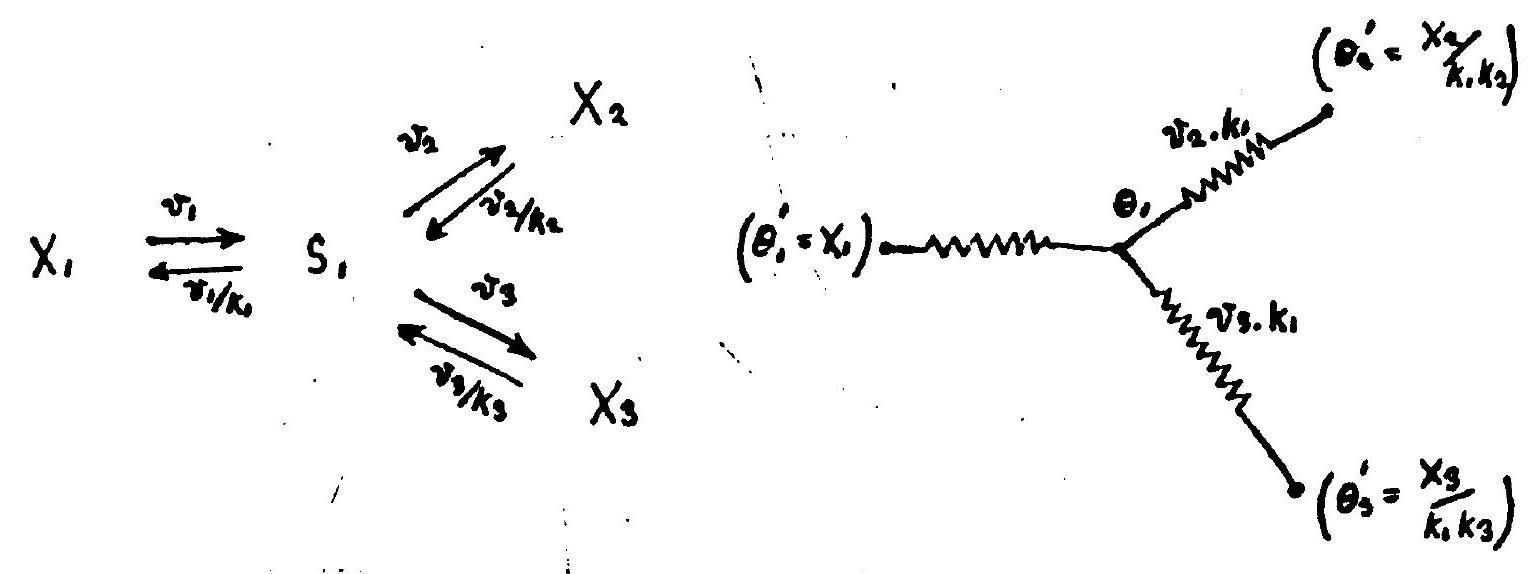
\includegraphics[max width=\textwidth]{2023_01_30_a974a42f7b7381f3f940g-051}
\end{center}

%\begin{center}
%
\includegraphics[max width=\textwidth]{2023_01_30_a974a42f7b7381f3f940g-051(1)}
%\end{center}

The fixed voltages $\theta^{\prime}$ are found from the fixed chemical concentration by the appropriate scaling. The sum of the current leaving the branch point must be zero, so that

$$
\begin{aligned}
& \left(\theta_{1}-\mathrm{X}_{1}\right)+\left(\theta_{1}-\frac{\mathrm{X}_{2}}{\mathrm{K}_{1} \mathrm{K}_{2}}\right) \cdot v_{2} \mathrm{K}_{1} + \left(\theta_{1}-\frac{\mathrm{X}_{3}}{\mathrm{K}_{1} \mathrm{K}_{3}}\right) \cdot v_{3} \cdot \mathrm{K}_{1} = 0 \\[5pt]
& \text { or } \theta_{1} = \frac{X_{1} v_{1} + X_{2} v_{2} \bigg/ K_{2} + X_{3} v_{3} \bigg/ K_{3}}{v_{1} + v_{2} K_{1} + v_{3} K_{1}}
\end{aligned}
$$
%
hence, for example, the flux in the 1st enzyme being numerically identical to the electrical current is
%
$$
\overline{F}_{1}=v_{1}\left(X_{1}-\theta_{1}\right) = v_{1}\left(\frac{X_{1}\left(v_{2} K_{1}+v_{3} K_{1}\right)-X_{2} v_{2} \bigg/ K_{2}-X_{3} v_{3} \bigg/ K_{3}}{v_{1}+K_{1} v_{2}+K_{1} v_{3}} \right)
$$
%
If each pathway had contained several enzymes it would only have been necessary to replace the conductances $v_{1}, \mathrm{K}_{1} v_{2}, \mathrm{K}_{1} v_{3}$ by the overall conductance possessed by, each pathway. These are found by the rule for summing a sequence of conductors which is that for example the four conductances where

\begin{center}
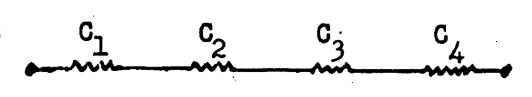
\includegraphics[scale=0.8]{figure1_conductance.png}
\end{center}

behave as one conductance $C$ where:
%
$$
1/C= 1/C_{1} + 1/C_{2} + 1/C_{3} + 1/C_{4}
$$
%
When applied to a straight chain this immediately yields an equivalent single conductance of value
%
$$
C = 1 \bigg/ \frac{1}{v_{1}} + \frac{1}{K_{1} v_{2}}+\frac{1}{\mathrm{K}_{1} \mathrm{K}_{2} v_{3}} + \cdots
$$
%
an expression which was involved in the flux through a straight chain studied earlier.

\section{Stability}

The property of dynamical stability is still possessed by the general network of reactions just discussed and this can be proved in a very general way. Thus in the equivalent electrical network the rate of dissipation of energy in a single conductance is current $x$ voltage or $\rho_{ij}\left(\theta_{i}-\theta_{j}\right) \times\left(\theta_{i}-\theta_{j}\right)$ and the total rate of dissipation, $L_{,}$in the network is given by
%
\begin{equation}
L = \sum \rho_{ij}\left(\theta_{i}-\theta_{j}\right)^{2} + \sum \rho_{iq}^{\prime}\left(\theta_{i}-\theta_{q}^{\prime}\right)^{2}
\label{eqn:122}
\end{equation}
%
where the summation is over all conductors. It can easily be verified that
%
$$
\begin{aligned}
& \frac{\partial L}{\partial \theta_{1}}=2 \sum_{j \neq i} \rho_{i j}\left(\theta_{i}-\theta_{j}\right)+2 \sum \dot{\rho}_{iq}^{\prime}\left(\theta_{i}-\theta_{q}^{\prime}\right) \\
\end{aligned}
$$
or using \eqref{eqn:121}
%
\begin{equation}
\frac{\partial_{L}}{\partial \theta_{i}}=-2 \eta_{i} \dot{\theta}_{i}
\label{eqn:123}
\end{equation}
%
Now when the system is in motion
%
$$
\dot{L} = \sum \left(\frac{\partial L}{\partial \theta_{i}}\right) \cdot \dot{\theta}_{i}
$$
%
or from \eqref{eqn:123}
%
\begin{equation}
\dot{L} = -2 \sum \eta_{i}\left(\dot{\theta}_{i}\right)^{2}
\label{eqn:124}
\end{equation}
%
Inspection of \eqref{eqn:122} and \eqref{eqn:124} shows that throughout any motion $L \geqslant 0$ and $\dot{L}<0$. Which implies that the dynamical system, when, released from any initial condition, can only move towards a stable stationary state. The results just established, equivalence to an electrical network and complete stability, apply to networks of linear unimolecular reactions and depend on the property that the product of equilibrium constants along different paths connecting the same metabolites is identical. This condition will also be satisfied in many networks of interest, which include `pseudo unimolecular' reactions provided these do not appear within any `cycle' of reactions.

By a `pseudo unimolecular' reaction is meant, for example, one of the form $A+B \rightleftarrows C+D$ but where $B$ and $D$. can be considered as parameters $B^{\prime}$ and $D^{\prime}$, that is as constant concentrations external to the dynamical system. In this case the true thermodynamic eq. constant $K_{E}=\left(\frac{C \times D^{\prime}}{A_{\times} B^{\prime}}\right)$ but since $B^{\prime}$, and $D^{\prime}$ are constant these will be an effective equilibrium constant $K_{E}$ for the pseudo-unimolecular reaction $A \rightleftarrows$ C. This constant is given by $K_{E}^{\prime}=K_{E} \times \frac{B^{\prime}}{D^{\prime}}$ and clearly is subject to no thermodynamic constraint. $\frac{B^{\prime}}{D^{\prime}}{ }^{\prime}$ being set at arbitrary level.

The \underline{general pseudo-unimolecular network} having linear rate expressions has no equivalent electrical network and correspondingly does not have the same simple solution and stability properties. However, even for this case there is a stability property which might be said to depend on the `conservation of molecules', found in all unimolecular systems. Thus in the equations \eqref{eqn:120}, for the general system, if the molar concentrations are measured as differences $S_{i}^{\prime}$ from the stationary values $\olsi{S}_{i}$ the equation of motion will be
%
\begin{equation}
\left[\begin{array}{c}
\dot{S}_1^{\prime} \\[5pt]
\dot{S}_2^{\prime} \\
\vdots \\
\end{array}\right]=\left[\begin{array}{l}
D
\end{array}\right]\left[\begin{array}{c}
S_1^{\prime} \\[5pt]
S_2^{\prime} \\
\vdots \\
\end{array}\right]
\label{eqn:125}
\end{equation}
%
where, for this linear system, the dynamical matrix $D$ has constant elements. A simple argument shows that these elements satisfy certain conditions. Suppose that all $S_{i}^{\prime}=0$ except one, say $S_{3}^{\prime}$, which is +ve then clearly, from the metabolic diagram and a consideration of the rate expression, $\dot{S}_{3}^{\prime}$ must be -ve and all other $\dot{S}_{i}^{\prime}$, re or zero, depending on whether they receive molecules from $\mathrm{S}_{3}$ or not. Furthermore, since all molecules leaving $S_{3}$ must arrive at other intermediate metabolites or leave the system, the sum of $\dot{S}_{3}^{\prime}$ and all other $\dot{S}_{i}^{\prime}$ must be $\leq 0$. Hence the matrix $D$ will have the form

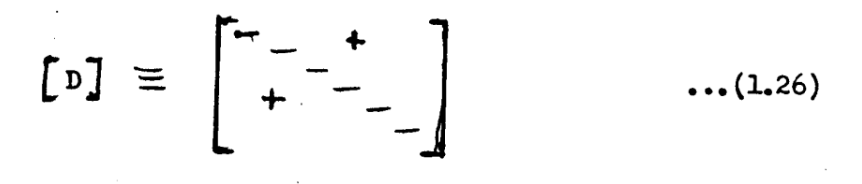
\includegraphics[scale=0.55]{figure1_1_26}

That is, -ve diagonal and all other elements +ve or zero. In addition D will satisfy the condition that in each column the sum of the elements is less than or equal to zero. These are sufficient conditions (HEARON, 1963) to ensure the stability of the system in the sense that although complex eigenvalues may occur their real parts will be -ve. This means that such systems may have a tendency to oscillate but that these oscillations will always be decaying.

In the case of networks not containing pseudo-unimolecular reactions within loops, it is always possible by suitably scaling the dynamical variables to symmetrise the matrix D, since this corresponds to the condition $\rho_{ij} = \rho_{ji}$ in (1.21). This further property of symmetrisability is sufficient to ensure that all eigenvalues of D are real (Hearon, 1963), so that such systems move towards their stationary solutions as a sum of decaying exponential terms. The straight chain mentioned earlier, whether it is truly unimolecular or not, is an example of this.

An example of a network, in which we are interested, containing potentially oscillatory cycles is the arginine cycle, indicated below.

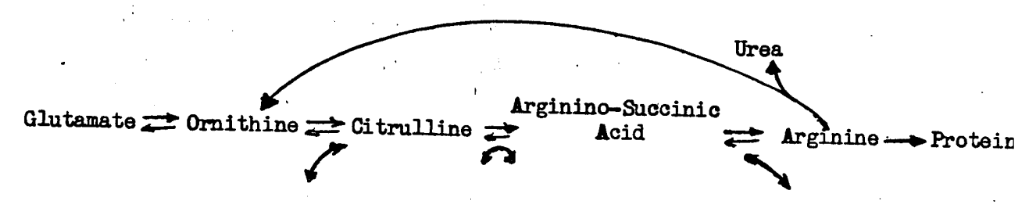
\includegraphics[scale=0.7]{figure1_argpathway}

Here several of the reactions within the cycle involve other metabolites. Even if these are treated as constant, so that the system is unimolecular, the fact that the product of equilibrium constants around different sides of the loop is not the same cannot be ignored. However, the general property proved above indicates that when the arginine system is approximated by linear rate-expression it will have just one stable solution, possibly arrived at via decaying oscillations.

The situation when the rate expressions for reactions in a unimolecular network are non-linear is of interest. In this case there will still be a set of equations similar to (1.25) for movement about the stationary state, but they will only apply for small disturbances from the $\olsi{S}_i$ and the elements of D will become the $\left[\frac{\partial \varphi_i}{\partial S_j}\right]_{S_j=\olsi{S}_{j}}$, discussed earlier.

However, the argument that (D) had the general form (1.26) and that its columns satisfied the required inequalities assumed only `conservation of molecules', which of course is still true, and that the rate expressions were restricted to have certain properties. The required properties are that they should involve only their own substrates and products and that when the level of a metabolite is increased its net rate of removal by a given enzyme should respond positively in the algebraic sense. Such properties are fairly general and will certainly be possessed by the simple rate-expression of (1.13b) allowing for saturation. Thus it is still possible to state, subject to this restriction, that the general network of non-linear unimolecular reactions will be stable, with decaying oscillations, in the neighbourhood of a stationary solution. For example if the arginine cycle were represented by nonlinear rate-expressions it would still be stable. However for true unimolecular networks with cycles the introduction of a saturable rate expression within a cycle could alter the type of stable dynamical behaviour, since the matrix [D] will no longer be symmetrisable.

With the introduction of non-linear rate expressions it becomes possible to represent `end product inhibition' and this is indicated below.

\begin{center}
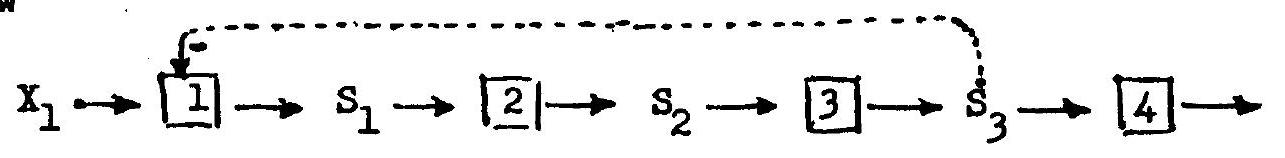
\includegraphics[max width=\textwidth]{2023_01_30_a974a42f7b7381f3f940g-057}
\end{center}

The rate expression for the 1st reaction, in this case, involves $\mathrm{S}_{3}$. Under these circumstances the system may become unstable since there are now off-diagonal -ve elements in [D]. Increasing the `strength' of the feedback corresponds to increasing the magnitude of the off-diagonal element and at some point the previously stable system will become unstable. However, because of the inherent stability of the initial system, a considerable feedback signal can be tolerated without instability. The stability of such systems has been treated subject to a number of simplifying assumptions (Walter, 1969).

\section{Nonlinear systems}

Turning now to the problem of locating the stationary state for a non linear unimolecular system it is clear that there will be no simple algebraic method since we now have a set of simultaneous non linear equations. The simplest case to consider is that of a straight chain of reactions where each enzyme has a rate-expression of the form (1.13b). This situation corresponds to the sequence of linear reactions discussed on p. 16 except that the fluxes per unit volume of the system become
%
\stepcounter{equation}
\begin{equation}
F_{i} = \frac{v_{i}}{\vecur{M_{i}}}\left(S_{i-1} - \frac{S_{i}}{K_{i}}\right) \big/ \left(1 + \frac{S_{i-1}}{\vecur{M_{i}}} + \frac{S_{i}}{\vecul{M_i}}\right)
\label{eqn:127}
\end{equation}
%
Where $v_{i}$ is now the maximum velocity of the ith enzyme in the direction $S_{i-1} \rightarrow S_{i}$ and for unit volume of the system $v_{i}$ will be proportional to the concentration $E_{i}$ of the enzyme. The constants $\vecur{M_{i}}$ and $\vecul{M_{i}}$ are the appropriate Michaelis constants and $K_{i}$ is the `effective' equilibrium constant for the step. Once again there are $n+1$ linear equations in $S_{1}, S_{2} \cdots S_{n}$ expressing the fact that at the stationary state the $n+1$ separate fluxes are all equal to the pathway flux $\olsi{F}$ These are obtained by multiplying up the denominator in expressions of the form (1.27) and yield.

%\section{$37 \cdot$}
\begin{center}
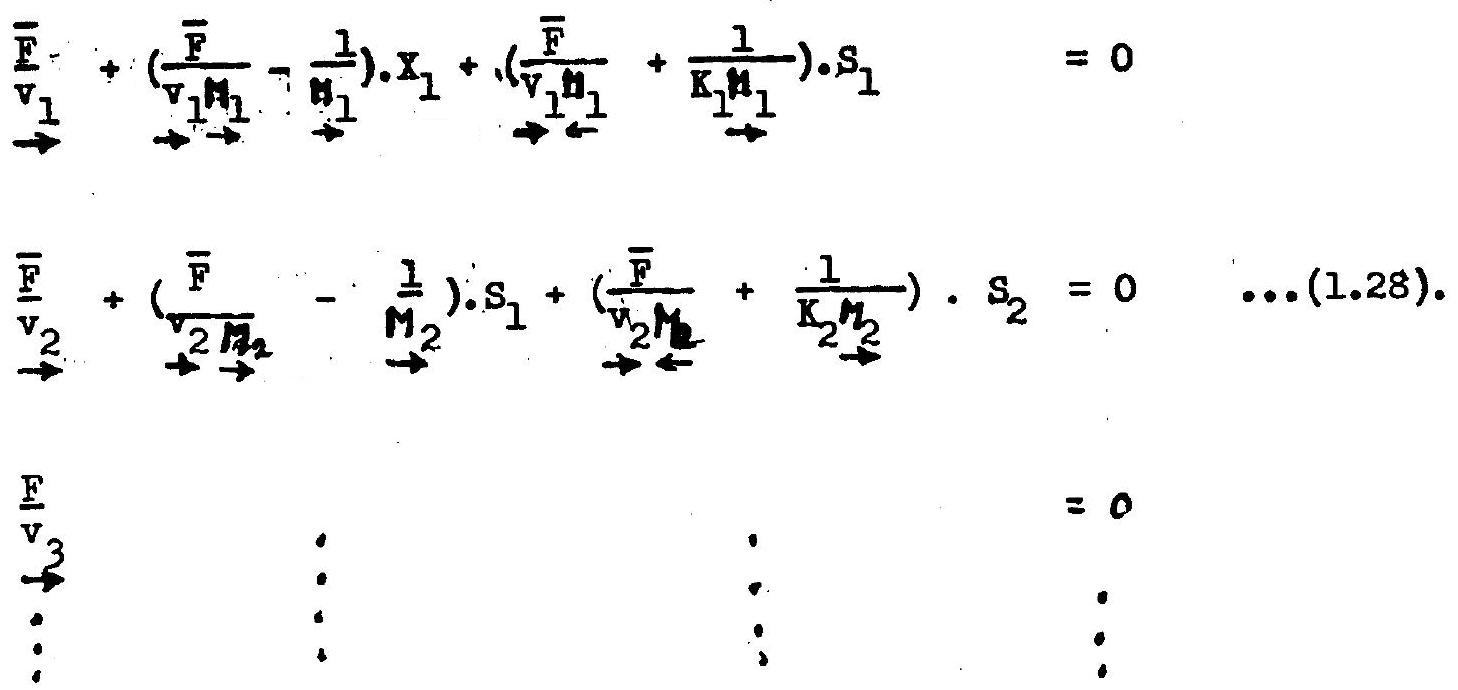
\includegraphics[max width=\textwidth]{2023_01_30_a974a42f7b7381f3f940g-059}
\end{center}

As before there are $(n+1)$ equations to determine only $n$ unknowns that the determinant of the coefficients must be zero or,

\begin{center}
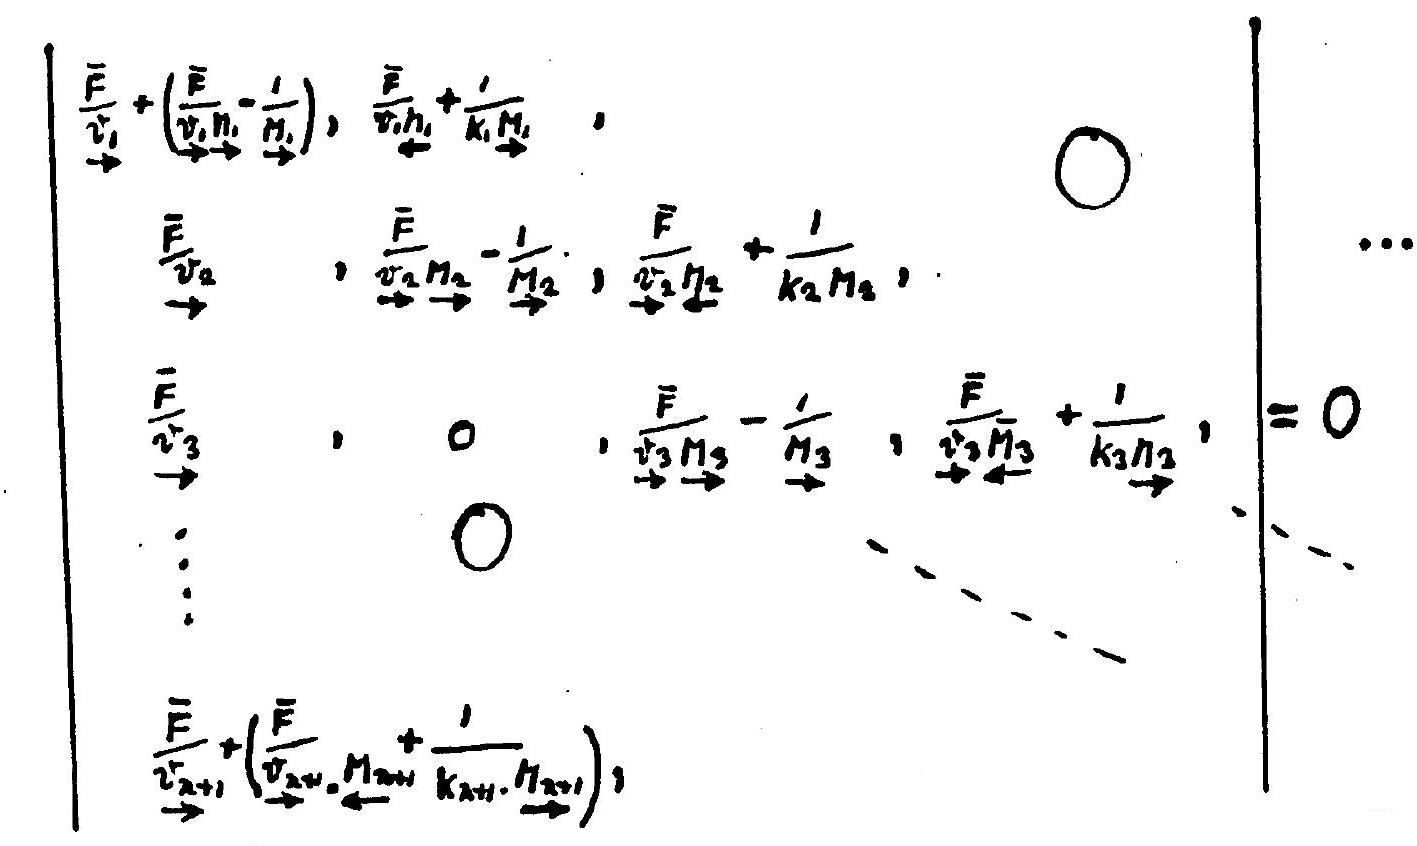
\includegraphics[max width=\textwidth]{2023_01_30_a974a42f7b7381f3f940g-059(1)}
\end{center}

The pathway flux, $\olsi{F}$, must satisfy the determinental equation, but $\olsi{F}$ now occurs in all elements of the determinant whereas formerly, in the linear case, it was present only in the first column. Consequently the equation of which $\olsi{F}$ is a solution is now a polynomial in $\olsi{F}$ of order $n+1$. Thus for two enzymes $\olsi{F}$ is one of the roots of a quadratic equation and for 10 enzymes it is one of the 10 roots of the 10th order equation. In fact it turns out that in this system there is never more than one $\olsi{F}$ satisfying the condition that all $\olsi{S}_i$ should be real and +ve. One consequence of $\olsi{F}$ being the solution of a high order equation is that there will no longer be an explicit formula, corresponding to (1.18) of the linear case, giving $\olsi{F}$ in terms of the parameters. Nor is it any longer the case that the overall action of a sequence of enzymes is equivalent to one enzyme. It appears then that when non-linear rate expressions are introduced, even in the simple case of a straight chain, there is no alternative but to study possible to investigate the `non-linear straight chain' problem algebraically with respect to the question of `diagnosing' from the pool pattern which steps in the chain are rate controlling. This question will be returned to in CH II, at the moment it will be show that even though there is no explicit expression for the flux it is still true that $\sum \mathrm{C}_{v_i}^{\olsi{F}}=1$. This can easily be seen by noting that in the functional relationship existing between $\olsi{F}$ and $v_{i}$.
%
$$
\olsi{F} = \olsi{F}\left(v_1, v_2, \ldots v_{2+1}\right)
$$
Thus simultaneous changes in the $v_i$ will cause a small change in $\olsi{F}$ according to
%
\stepcounter{equation}\stepcounter{equation}
\begin{equation}
\delta \olsi{F}= \sum \frac{\partial \olsi{F}}{\partial v_{i}} \cdot \delta v_{i}
\label{eqn:130}
\end{equation}
%
Now inspection of the determinant (1.28) shows that if all $v_{i}$ are increased by the same factor $(1+a)$ then $\olsi{F}(1+a)$ will be the new solution. So that changes $\alpha v_{1}, \alpha v_{2}, \dots$ produce a change $\alpha \olsi{F}$ in the flux. When $\alpha$ is small this can be substituted in (1.30) and

$$ \alpha \olsi{F} = \sum_i \frac{\partial \olsi{F}}{\partial v_i} \cdot \alpha v_i $$
%
or
%
\begin{equation}
1 = \sum \frac{v_i}{\olsi{F}} \cdot \frac{\partial \olsi{F}}{\partial v_i} = \sum C_{v_i}^{\olsi{F}} 
\label{eqn:131}
\end{equation}
%
Thus it appears that the summation property of rate control coefficients, originally proved for the linear case, may be a fairly general one.



\chapter{Mathematical Formulation of Complex Systems}

In the last chapter, after a general theoretical section, unimolecular systems were considered in some detail. It was shown that, even for such unimolecular systems, explicit solutions for the stationary state could not be obtained, except for the hypothetical `completely linear' case. However, it was seen that the concepts of `rate-control' and `diagnostic' could give a useful insight into the workings of systems, even when there was no explicit solution. For the more complex systems, whose representation is to be considered in this chapter, the necessity of understanding a system by considering its response to parametric variation is even greater, since very little in the way of analysis can be achieved.

When the variation is differential the response of the system will be expressed naturally by a `sensitivity coefficient matrix' and in CH. III the theoretical basis of this will be developed with particular reference to how it is related to the properties of individual enzymes and how it can be estimated experimentally.

The response to finite parameter variation can only be studied by means of numerical experiments performed on mathematical models. In CH. IV a computer system capable of flexibly performing such `in numero' experiments on a variety of general systems is discussed.

The contents of this chapter will, then, be concerned with the problem of formulating complex metabolic systems. in the mathematical terms suitable to computer analysis. After discussing the distribution between a `subsystem' and a `complete' system and initially restricting consideration to subsystems, the network of genial reactions is introduced.

This lifts the previous restriction to unimolecular reactions and in addition allows the representation, via suitably complex rate expressions, of `allosteric' enzymes, where substances can influence the rates of reactions from which they are metabolically remote. Next it will be shown that, for systems where it is wished to consider the effects of substituting alternative alleles for structural genes, a new type of genotypic parameter can be introduced by extending the idea of a `rate expression'. The section ends by considering how the effects of 'growth' and 'enzyme regulation' may be represented for subsystems.

Finally an approach is made to the problem of formulating `complete systems', which gives consideration to the allocation of resources by differential gene activity.

\section{Subsystem and complete system}

An dynamical system of the type which was discussed in CH.I (1.1) involves the assumption that some metabolites, denoted by $S_{1}, S_{2} \cdots,$ are \underline{within} the system and are variables, whereas others $X_{1}, X_{2} \cdots$, are \underline{outside} the system and have the status of parameters. The assignment of any metabolite to one of these two classes is clearly a quantitative judgement and has up till now been made on the reasonable basis that the medium had a relatively large volume and approximated to an infinite source or sink, thus rendering the concentration environmental metabolites almost constant. However the assignment is clearly arbitrary and cannot de applied in certain situations, where it becomes necessary to widen the system so as to include at least some `environmental metabolites as variables, for example if it is wished to consider `growth in a chemostat.

Even when the environmental metabolic boundary can be accepted a difficult problem arises because of the necessity of reducing the large number, many thousands, of metabolites which are involved in a `real' system. One way in which this reduction can be performed, for our stationary state studies, is by eliminating system variables which are not directly of interest, a technique which has already been used to eliminate unwanted enzymic intermediates. However, this was possible only because, on the assumption that protein-protein interaction was negligible, the necessary eliminations involved only linear equations in the enzymic intermediates and were already fully treated under the subject of steady state enzyme kinetics. The equivalent technique at the level of intermediary metabolites is not in general possible because non-linear equations are involved. For example it might involve eliminating metabolites within a sequence of enzymes and replacing the sequence by a single `enzyme' with a complex rate expression, a task which, as was seen in CH I, has no explicit algebraic solution. Hence, in general, no such exact reduction can be made. It may, however, prove possible to find closed algebraic expressions which are a reasonably good description of pathway behaviour, provided that the remaining system variables lie within certain ranges.

In these circumstances it is necessary to view the problem of reduction in a flexible way; 'what is a reasonable reduction in one situation may be quite unreasonable in another. One extreme is the situation when the parameter changes being studied are likely to have large effects throughout the whole metabolic system, even though the varied parameters may themselves all be within one pathway. Changes which, for example, markedly affected growth rate would seem to be of this type. In this case there is no escape from considering some representation of the `complete' system . The representation being, perhaps, detailed only in the region of the parameter changes, it being sufficient elsewhere to represent the functioning of whole areas of metabolism, as for example the glycolytic pathway, in some approximate way. Some consideration will be given to the rather difficult problem of such complete systems at the end of this chapter.

Another way in which the desired reduction can be made is to consider the area of metabolism in which parameter variation is to be made as a `sub-system'. This involves arguing that internal metabolites which are `remote' from the sub-system will remain more or less constant and can be formally treated as `external' metabolites.

The criteria for deciding what constitutes such a sub-system are not simple. The correct decision is clearly a quantitative matter and will depend, inter alia, on the size of the parameter variations. In general, the larger the variation the larger will have to be the sub-system. Despite the difficulty in defining exactly what is meant by a subsystem, in this sense, there is no alternative but to use the concept.

\section{Network of general enzymically catalysed transformations}

Until now we have considered systems of effectively unimolecular reactions, where the transformations, taking place within a fixed volume, are represented in a system diagram by steps of the type:

\centerline{
\includegraphics[scale=1]{figure2_pathway10.png}}

This means that the 10th enzyme catalyses a unimolecular conversion from $S_{a}$ to $S_{b}$ in the sense that for every molecule of $S_{a}$ removed one of $S_{b}$ is produced. The net-flux/unit quantity of enzyme, taken as +ve in the arrowed direction, was given by a rate-expression which assumes enzymic intermediates to be at a stationary state with respect to $S_{a}$ and $S_{b}$ and which takes fully into account that the reaction $S_{a} \longrightarrow S_{b}$ can be reversible.

This can easily be generalised to allow for enzymically catalysed reactions of arbitrary complexity. For example the reaction
%
\begin{equation}
S_a + S_b \rightleftarrows S_c + 2 S_d
\label{eqn:21}
\end{equation}
%
is symbolised by

\centerline{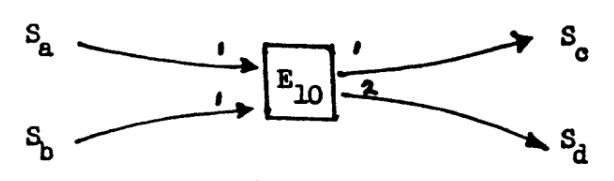
\includegraphics[scale=0.65]{figure2_E10.png}}

and has a rate-expression/unit quantity of enzyme giving the net flux towards, say, the metabolite $S_{c}$ of $f_{10}\left(S_{a}, S_{b}, S_{c}, S_{d}, \ldots.\right)$. Clearly the corresponding rate expressions for the metabolites $S_{a}, S_{b}, S_{d}$ are $-f_{10},-f_{10}$, and $+2 f_{10}$ respectively where the appropriate stoichiometric constants $-1,-1,2$ are obtained from the equation (2.1) for the net reaction. The symbol $f_{10}$ stands here for either the function or its value, depending on the context.

In a general network of reactions, if $f_j$ is the rate expression for unit quantity of the jth enzyme referred to one of its products, then $\lambda_{ij} f_j$ will be the appropriate rate expression of the $j$th enzyme for the ith metabolite.

The \underline{`stoichiometric matrix'} $\left[\lambda_{ij}\right]$ will consist of small integers, mostly 1 and $-1$, and zeros and will in fact contain mostly zeros, since most enzymes remove or produce only a few metabolites. In a system having $n$ metabolites and $m$ enzymes $\left[\lambda_{i j}\right]$ will be an $n \times m$ matrix.

The figure below represents a general system existing in a given volume $V$ and with total quantity, $\mathrm{E}_j^T$ of the jth enzyme. This can be distributed in any way throughout the volume or, if a transport enzyme, upon the surface.

\centerline{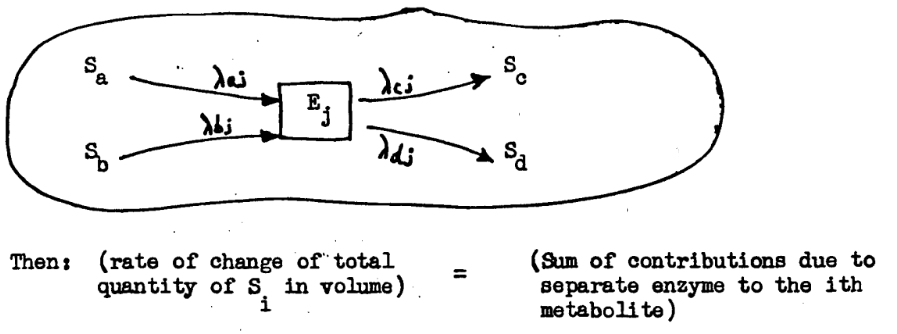
\includegraphics[scale=0.8]{figure2_1.png}}

%Thenr (rate of change of total $=$ (sum of contributions due to quantity of $S_{i}$ in volume). separate enzyme to the ith metabolite)

\begin{figure}
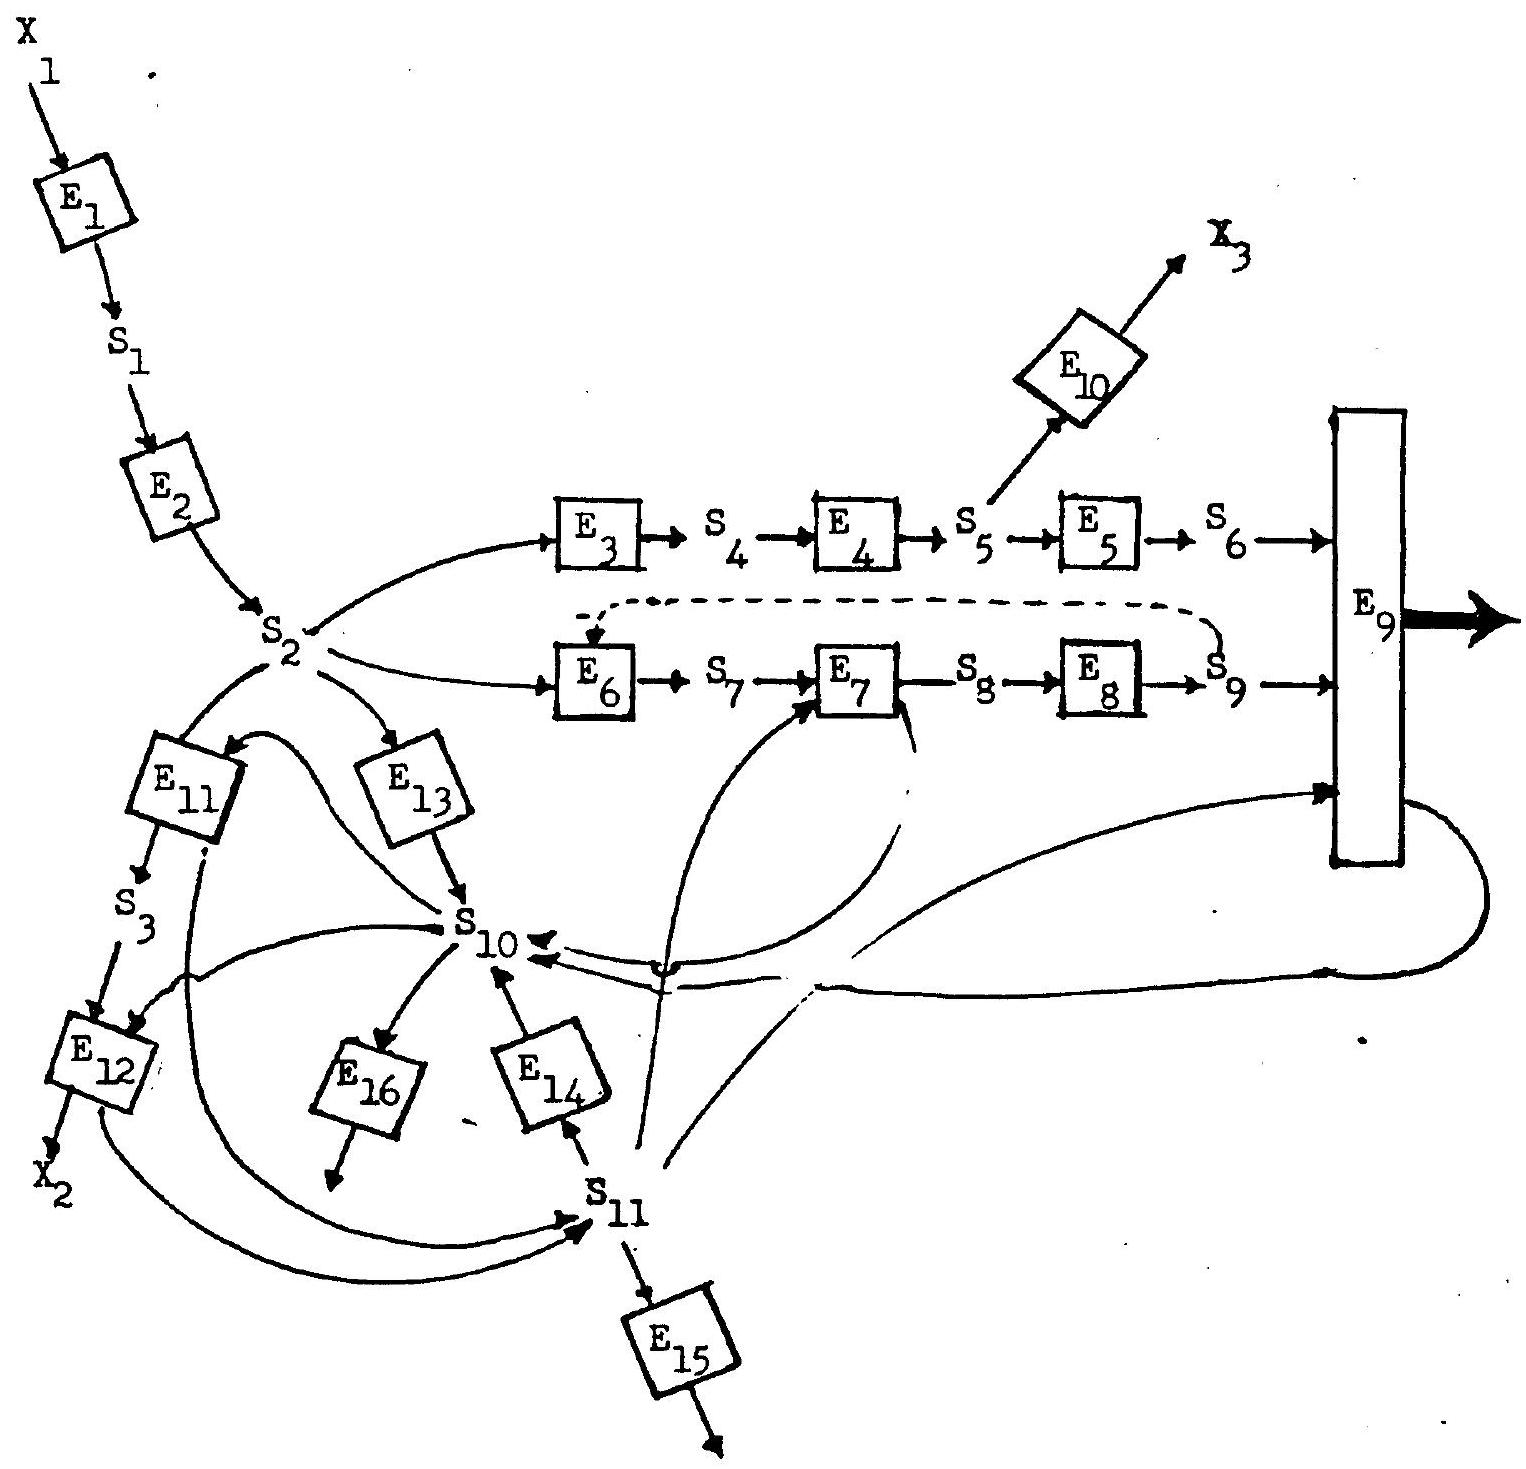
\includegraphics[scale=0.2]{2023_01_30_a974a42f7b7381f3f940g-068}
\caption{METABOLIC STRUCTURE}
\end{figure}

\begin{figure}
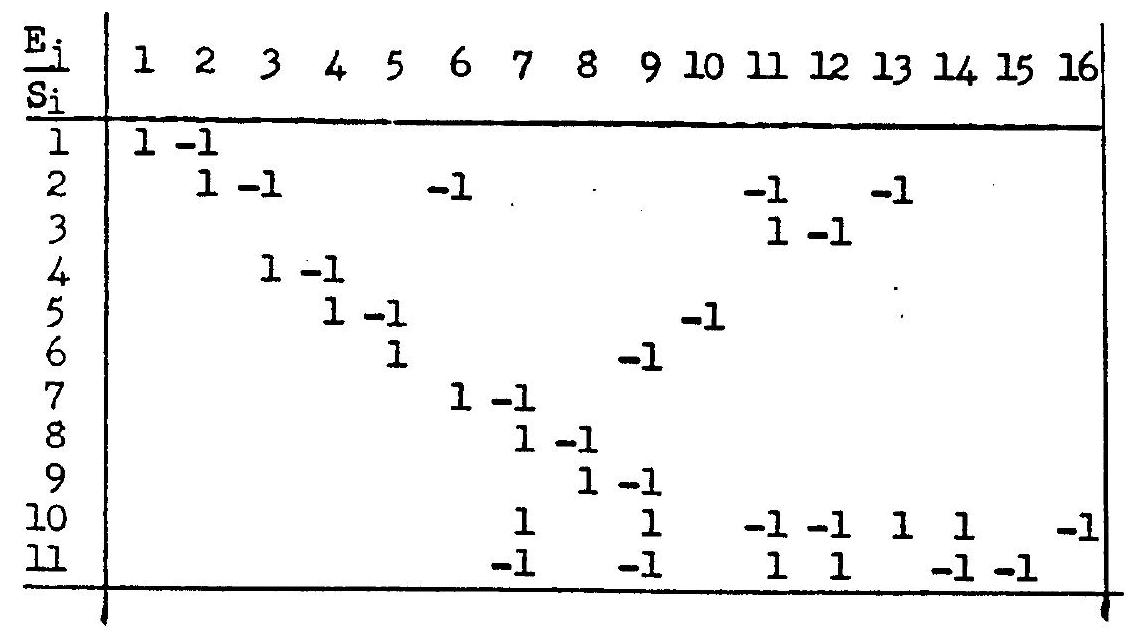
\includegraphics[scale=0.25]{2023_01_30_a974a42f7b7381f3f940g-068(1)}
\caption{STOICHIOMETRIC MATRIX}
\end{figure}

\begin{equation}
\frac{d (S_i \times V)}{dt} = \sum_j \lambda_{ij} E_{j}^{T} f_{j}(\ldots)
\label{eqn:22}
\end{equation}
%
or
%
$$
\dot{S_i} =\quad \sum \lambda_{i j}\left(\frac{E_{i}^T}{V}\right) \cdot f_{j} - \left(\frac{1}{V} \dot{V}\right) \cdot \dot{S}_{i}
$$
%
Writing $\frac{E_{j}^{T}}{V}=E_{j}$ the effective concentration of the jth enzyme in the system and remembering that  ($1/V \dot{V})=0$ we have the dynamical functions $\varphi_{i}$ for the general system as
%
\begin{equation}
\varphi_{i}=\dot{S}_{i}= \sum \lambda_{i j} E_{j} f_{j}(\ldots)= \sum \lambda_{ij} F_{j}
\label{eqn:23}
\end{equation}
%
In (2.3) $\mathrm{F}_{\mathrm{j}}$ is the net flux carried by the $\mathrm{jth}$ enzyme in unit volume of the system, the flux being defined by reference to one of the substrates of the $j$th enzyme.

The general equation (2.3) will be made more concrete by means of an example, shown in fig (1), which will illustrate how various metabolic situations can be represented. This example will also be used to discuss certain conditions to which the equations (2.3) must conform.

The metabolic network of fig (1) comprises 16 enzymes, 10 intermediate metabolites and four external substances and the general meaning of the metabolic scheme is as follows. $X_{1}$, which can be regarded as a nutrient, is transported in an converted to $S_{2}$ at which point the metabolism divides into several pathways. A catabolic pathway, $S_{2} \rightarrow S_{3} \rightarrow X_2$, yields a high energy product $S_{11}$ by bimolecular coupling reactions at steps 11 and 12. Two biosynthetic pathways, $\mathrm{S}_{2} \rightarrow \mathrm{S}_{4} \rightarrow \mathrm{S}_{5} \rightarrow \mathrm{S}_{6}$ and $\mathrm{S}_{2} \rightarrow \mathrm{S}_{7} \rightarrow \mathrm{S}_{8} \rightarrow \mathrm{S}_{9}$ converge onto a condensing reaction at step 9, the second of these pathways and the condensing reaction being coupled to the high energy product $\mathrm{S}_{11^{*}}$

Clearly $S_{10}$ and $S_{11}$ have a similar role to that of ADP and ATP in a real system and the step $\mathrm{E} 9$ would correspond to protein synthesis. Continuous lines represent a net flux of metabolite, whilst the arrow and the number above it indicate the algebraically positive direction and stoichiometric constant respectively. Dotted lines indicate metabolites influencing the rate of a reaction, without themselves being appreciably consumed, the sign above the arrow indicating, when appropriate, whether there is an inhibitory or excitatory effect. Thus in the figure it can be seen that $S_{9}$ exerts feedback inhibition on $E 6$ the last enzyme in its own pathway, or again the external substance $X_{4}$ activates the last enzyme in the same pathway. All these effects are taken fully into account by multiplying the stoichiometric matrix $\lambda_{i j}$, shown below the figure, into the set of rate expressions, $f_{1}, \cdots, f_{16}$ to produce the 10 functions $\varphi_{1}, \cdots, \varphi_{10}$ The dynamical functions can then be used, as explained earlier, to obtain the stationary solution and the sensitivity of any measures to any parameters which are of interest. Thus the problem of describing the system mathematically is just that of writing dorm the set of rate expressions, $f$. How exactly this is done will depend on what qualities are considered to be possessed by the separate enzymes. For instance the unimolecular expressions $f_{1}, f_{2}$ may simply be of the usual linear form (1.13b) unless it is suspected that their saturation properties are important. Other expressions clearly have to be more complex just to represent the effects encoded in the metabolic diagram. For example, the simplest possible rate-expression for the bimolecular reaction of $\mathrm{E}_{11}$ would be
%
$$
f_{11}(\ldots .)=k_{x}\left(S_{2} \times S_{10} - S_{3} \times S_{11} /K_{10}\right)
$$
%
and this, of course, takes no account of saturation effects. Again there are various possibilities for representing $\mathrm{E} 6$, which is sensitive to feedback inhibition from $S_{9}$, one of the simplest being
%
$$
f_{6}(\ldots)=k_{1 x}\left(S_{2} - \frac{S_{7}}{K_{6}}\right) \times \frac{1}{\left(k_{2} + S_{9}\right)}
$$
%
The situation then is that metabolic `structure' of considerable detail can be included in the functions $\varphi_{1}, \cdots, \varphi_{10}$ by means of the matrix $\left[\lambda_{i j}\right]$ and the set of rate-expressions. In general these rate expressions should be of the simplest form which will express the desired properties of the separate enzymes, However, the general set of equation $(2.3)$ must satisfy a certain condition as will be discussed in the next section.

\section{Necessity for linear independence of the functions}

This arises because if it happens that one of the $\varphi_i$ is simply a linear combination of others there will not be sufficient simultaneous equations to determine the stationary solution. Since the rate expressions are clearly all independent functions this condition of linear independence is just that the rows of $\left[\lambda_{ij}\right]$ be linearly independent.

An example will show how faulty formulation of a set of equations may generate dependence. In formulating a system involving, say, a set of ADP/ATP dependent reactions, it might be thought sufficient to link the generating system to the absorbing system by a closed loop. In terms of our model fig (1) this is equivalent to omitting the steps E13 (generation ADP), E15 (degrading ATP) E16 (degrading ADP). This might appear to satisfy the linked steps E11 and E12.

The rates of change of the two substrates, $S_{10}$ and $S_{11}$ would then be:
%
$$
\begin{aligned}
\dot{S}_{10} &= \varphi_{10}=-F_{11}-F_{12}+F_7+F_9+F_{14} \\
\dot{S}_{11} &= \varphi_{11}=+F_{11}+F_{12} - F_7-F_9-F_{14}
\end{aligned}
$$
%
For the stationary state conditions we find that $\varphi_{10}=0$, implies that $\varphi_{11}$ is determined also to be zero and imposes no separate condition. This eliminates one of the $n$ necessary equations for solution. Dynamically the system would have the property $\frac{d\left(S_{10}+S_{11}\right)}{dt}=0$ so that the sum of ATP and ADP could not change and would be dependent on the initial conditions (viz, the initial value of the sum). In addition the matrix $D=\left[\frac{\partial \varphi_{i}}{\partial S_{j}}\right]$ would have no inverse thus invalidating the iterative method of (1.9). A biochemical system formulated in this way would thus not have the property that the stationary state was dependent only on genetic and environmental parameters, and the whole theoretical approach outlined earlier would be invalid.

It seems reasonable to argue that this difficulty arises out of the unreality of formulating a system in which production of ATP is always coupled to removal of ADP and vice versa. The solution of the difficulty then is to extend the system by adding the reactions E13, E15, E16, which allow $\mathrm{S}_{10}$ and $\mathrm{S}_{11}$ to participate in non-coupled reactions and thus renders $\varphi_{10}$ and $\varphi_{11}$ linearly independent.

It may be objected that the investigator wishes to consider a situation where the sum of ATP and ADP is at a previously prescribed level. This is of course still possible with the extended model. The difference being that instead of the sum being determined by initial conditions it must now be determined by parameter values acting within the system. For example, suppose the reaction El3 is an irreversible reaction saturated by $S_{2}$ and providing a flux/ unit volume determined by a parameter $k_{1}$ and that E16 and E15 are linear and irreversible with the same effective rate constants $k_{2}$ Then at S.S.,
%
$$
\varphi_{10}=-F_{11}-F_{12}+F_{7}+F_{9}+F_{14}+k_{1}-\left(k_{2} \times \olsi{S}_{10}\right) = 0
$$
%
and $\varphi_{11} = -\mathrm{F}_{11}-\mathrm{F}_{12}+\mathrm{F}_{7}+\mathrm{F}_{9}+\mathrm{F}_{14}+\mathrm{k}_{1}-\left(\mathrm{k}_{2} \times \olsi{\mathrm{S}}_{11}\right)=0$ so that
%
$$
\left(\olsi{S}_{10} + \olsi{S}_{11}\right) = k_{1}/k_{2}
$$
%
Therefore by adjusting the parameter $k_{1}$ the investigator can prescribe the sum of ATP and ADP.

In general then only systems, having the property that the rows of $\left[\lambda_{ij}\right]$ be linearly independent, will be considered, additional reactions being added if the condition is not at first satisfied. This will ensure the applicability of the mathematical methods outlined earlier for calculating the sensitivity coefficients whilst not restricting the investigator in any important way.

\section{Independent fluxes in a system}

An important `measure' in a system is often the stationary flux/unit vol, $\olsi{F}_{j}$, at some step in the network, there being $m$ such measures in a system having $m$ enzymes. However, these stationary fluxes are not independent since there are $n$ conditions connecting them, namely
%
\begin{equation}
\varphi_{i}=\sum \lambda_{i j} \olsi{F}_{j}=0 \mbox{ For } i=1 \mbox{ to } n
\label{eqn:24}
\end{equation}
%
The number of independent fluxes will thus be the number of enzymes less the number of conditions connecting them or $(m-n)$.

For example, in a straight chain the number of enzymes will only be one more than the number of pools and hence there is just one independent or `pathway' flux.

For the more complex system of fig (1) there are 16 enzymes and 11 pools so that there are 5 independent fluxes. This means that if 5 selected fluxes are known the remaining 17 can be found using the condition (2.4). This amounts to inverting part of the matrix and may appear algebraically complex. However, the connection between the fluxes can be seen immediately from a metabolic diagram. Thus, if the 5 excretory fluxes $F_{0}, F_{10}, F_{12}, F_{15}, F_{16}$, in fig(1) are selected as metabolically significant the other fluxes can be written down in terms of them as for example:
%
\begin{equation}
\begin{aligned}
& \olsi{F}_5=\olsi{F}_9 \\
& \olsi{F}_4=\olsi{F}_9 + \olsi{F}_{10} \\
& \olsi{F}_6=\bar{F}_9 \\
& \olsi{F}_{11}=\olsi{F}_{12} \\
& \olsi{F}_{13}=\olsi{F}_{16} + \olsi{F}_{15} \\
& \olsi{F}_2=2 \olsi{F}_9 + \olsi{F}_{10}+\olsi{F}_{12}+\olsi{F}_{16}+\olsi{F}_{15}
\end{aligned}
\label{eqn:25}
\end{equation}
%
For most metabolic systems the number of enzymes will only slightly exceed the number of metabolites so that in fact there are relatively few independent fluxes in a network.

\section{Introduction of genotypic parameters}

Suppose that in the 16 enzyme system of fig. (1) alternative enzymes were available at various steps in the network, then the particular set of enzymes possessed by such a 16 enzyme `organism' would depend on its set of alleles or its `genotype'. The introduction of a set of ``genotypic parameters'' ( $\pi_{1}, \pi_{2}, \cdots, \pi_{16}$ ) specifying. the allelic situation at each step. will serve to describe the genotype. For example in a haploid organism with two alleles at each locus the $\pi$ integers must each take one of two values, whereas if the organism were diploid there would be three possible values since at each locus there are, physiologically, three alternative states, Figure (2), homozygous either way and heterozygous.

\centerline{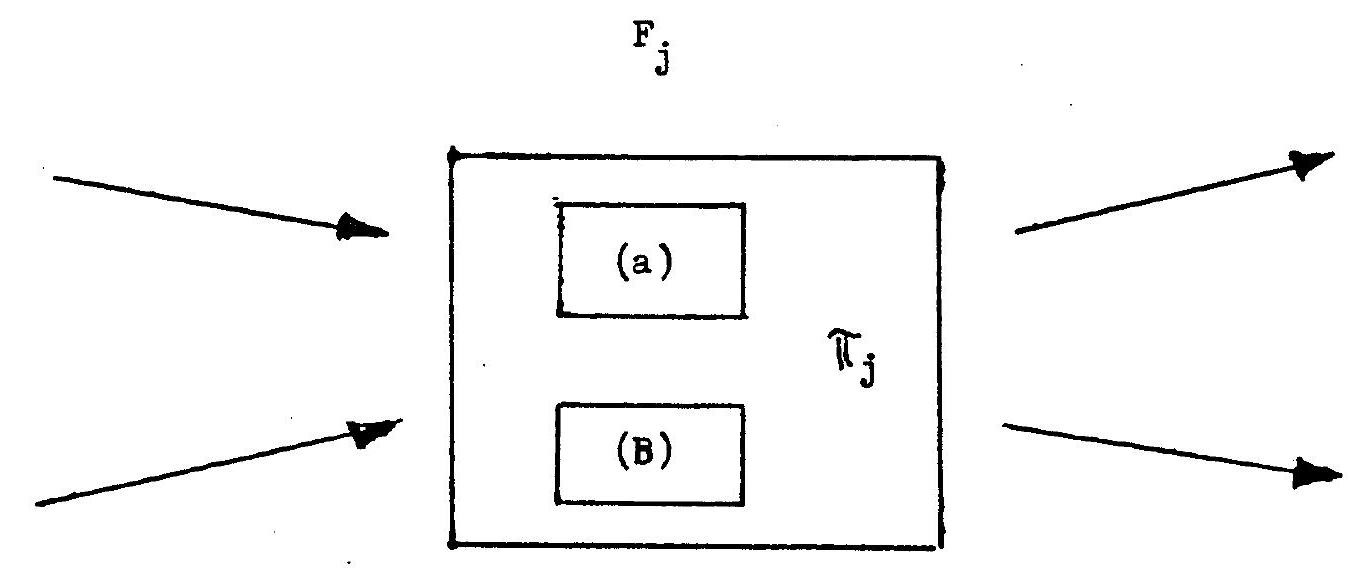
\includegraphics[scale=0.5]{2023_01_30_a974a42f7b7381f3f940g-076}}

The flux depends on the allelic enzymes $E_{j}^{a}$ and/or $E_{j}^{b}$. The $\pi$ value specifies the allelic state of the locus.

\begin{figure}
\centering
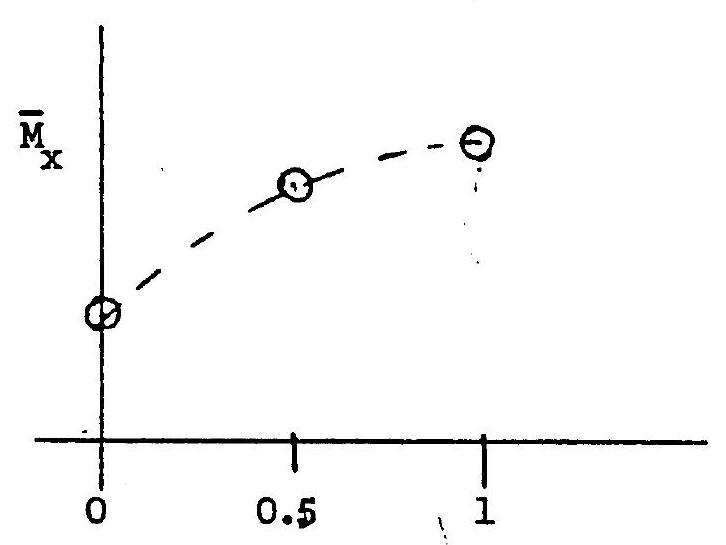
\includegraphics[scale=0.26]{2023_01_30_a974a42f7b7381f3f940g-076(1)}
\caption{The measure $\olsi{M}_{x}$ as a function of the value of $\pi$.}
\end{figure}

Consideration of the phenotype/genotype, or Ph/Ge relation will clearly be facilitated if these ir parameters can be included in the specification of the functions $\varphi_1 \cdots, \varphi_{n}$. This can conveniently be done by extending the idea of a rate expression, the new formulation depending on the ploidy and the number of alternative alleles at each locus. The case of two alternative alleles per variable locus will be considered for haploid and diploid organisms.

Thus for a haploid organism suppose that the alleles for the jth locus give alternative enzyme concentrations $\mathrm{E}_{j}^{\mathrm{a}}$ and $\mathrm{E}_{j}^{\mathrm{b}}$ and alternative rate expressions $f_{j}^{a}(\ldots)$ and $f_{j}^{b}(\ldots$) , it being noted that these expressions may be of quite different form as for example one being sensitive to end product inhibition and the other not. A composite expression (cf. Fig. (2)) can be written for the flux/unit volume at the jth step thus.
%
\begin{equation}
F_{j}=\left(1-\pi_{j}\right) E_{j}^{a} f_{j}^{a}(\cdots)+\pi_{j} E_{j}^{b} f_{j}^{b}(\cdots)
\label{eqn:26}
\end{equation}
%
and clearly $\pi_j = 0$ gives the (a) allele and $\pi_i = 1$ gives the (b) allele so that 0 and 1 are the possible values for $\pi^{j}$

Since the description is formally the same as before, only with a more complex set of rate expressions which involve the if $g$ the same numerical techniques will work. In particular it will be possible to consider how a measure $\olsi{X}$ depends on the set of alleles constituting the genotype since the non algebraic functional relationship
%
\begin{equation}
\olsi{M}_{X}=\olsi{M}_{X}\left(\pi_{1}, \pi_{2}, \ldots, \pi_{16}\right)
\label{eqn:27}
\end{equation}
%
can now be investigated numerically.

For a diploid organism it is only. necessary to allow the $h_{j}$ to take three values, $0,1/2,1$, where $\pi_{j}=1/2$ corresponds to the heterozygous state at the $j$th locus. This involves the assumption that enzyme quantity is proportional to gene dosage which seems reasonable so long as enzyme quantity is till treated as a genetically specified parameter. The response of a measure to $\pi_{j}$ indicated in fig. (2) now gives an indication of the importance and the degree of dominance of the $j$th locus and the effect on this of varying other $\pi_{j}$, that is the genetic background, can be tried.

The introduction of the or notation makes clearer what is meant by the Ph/Ge relation. It also reveals a difficulty not previously raised. Thus the_Ph/Ge response matrix $\left[\mathrm{C}_{\mathrm{P}_y}^{\mathrm{M_X}}\right]$ of (1.9) can now be recognised as $[C^{\olsi{M}_X}_{\pi_y}]$ but since ${\pi}_y$ can only assume discrete values the meaning and usefulness of the differential sensitivity analysis will have to be considered. The uses of the general relationship (2.7) in the framework of theoretical ! population genetics will be discussed in CH.V.

\section{Non-enzymic transformations}

In metabolism there will be many situations where non-enzymic transformations are important, e.g. in the case of surface transport by simple diffusion. These can be represented perfectly well using rate expressions the only difference being that instead of enzyme concentration there will be some other factor. Thus `non-enzymic transport' rate-expressions will involve the quantity area/volume, or $A/V$. That is the 'concentration of area' rather than the concentration of enzyme. Enzymically mediated transport expressions will not involve $A/V$ since the amount of surface over which the enzyme is distributed is not relevant. The inclusion of nonenzymic transformations will not alter the general form of (2.8) except that a new category of pseudo-enzymes are introduced.

\section{Expanding systems}

It is often of interest to consider growing systems, particularly since the condition of steady or exponential growth of a culture of such systems is a well defined experimental situation: such a growing system clearly does not possess a stationary state, since certain system parameters are no longer constant with time.(Grainger, 1966, 1968).

However, subject to the conditions that these parameters do not vary too rapidly or over too wide a range and that the system itself is intrinsically stable (see next section) the stationary state approach still proves useful.

Thus an investigator of such a non-stationary system would be interested in the mean values over time, $\left\langle S_{i}\right\rangle_{t_1}$ of system variables. Given the above conditions the $\left\langle S_{i}\right\rangle_{t}$ will be well approximated by the stationary $\olsi{S}_{i}$ corresponding to average values of varying parameters. In fact fluctuating parameters in a growling system are often quite well behaved In the above sense. For example in a spherical cell which continuously doubles its volume and then divides, perhaps representing a growing bacterium, the parameter (A/V) suffers a sharp increase of $\approx 25 \%$ at each division and then gradually falls to reach its former value just prior to the next division. Thus, given reasonable metabolic stability, the system will be close to a stationary solution during most of the time and will suffer its greatest disturbance at each cell division. A similar situation holds for the parameter combinations 'relative gene dosage', whose importance will be seen in the section on control. These double at certain points in the cell cycle when each gene is duplicated and decline steadily during the rest of the cycle due to other genes being replicated. For syncytial growth the stationary state assumption may be a very good approximation, thus (A/V) will vary hardly at all during the tube like growth of hyphae and the `relative gene dosage' will remain almost constant since in this case a number of asynchronously dividing nuclei inhabit a common metabolic space. Supposing then that it is acceptable to study the stationary state corresponding to average parameter values the effect of growth on this S.S. will still have to be allowed for. This arises because it is no longer permissable to assume $\dot{V}=0$ when simplifying the dynamic equations (2.2). Thus instead of the form (2.3) there arises

\begin{equation}
\varphi_{i}=\dot{S}_{i}=\sum \lambda_{ij} E_{j} f_{j}(\ldots)-(1/V \dot{V}) \cdot S_{i}
\label{eqn:28}
\end{equation}

Clearly a stationary. solution with growth will require all $S_{i}$ constant and $\dot{V} \neq 0$ and will only be possible if the term $(1/V \dot{V})$ is constant. This means that such growth will be exponential with growth constant $G$, where
%
$$
G = \frac{1}{V} \dot{V}
$$
%
Since, for the present, only `subsystems' are being considered $G$ has to be treated as a parameter. The equations (2.8) are then formally equivalent to a metabolic system within a fixed volume and having a ``flux to expansion'' of $G \times S_{i}$ away from each $S_{i}$. Whether these expansion terms will constitute more than a minor correction will depend on the metabolic pathways contained in the subsystem. In any particular case the G constant will, of course, be known and the problem in setting up the model is to assign levels to the $E_{j}$ consistent with general data.

For example in the arginine pathway it may be known that arginine in pool form is of the order of $5 \%$ of arginine in protein in which case the ${E}_{j}$ in arginine pathway would be adjusted until the terms $\lambda_{i j} E_{j} f_{j}(\ldots)$ are approximately twenty-fold greater than GS$_{\text {arg }}$. This involves some guesswork but can usually be done satisfactorily. The expansion terms can usually be ignored in major pathways such as the glycolytic, which carry a large flux, but may be of dominant importance in pathways carrying a small flux such as co-enzyme synthesis. In addition any mutants tending to block the flux in a pathway and at the same time raise the pool levels will enhance the importance of the expansion terms.

\section{Stability of networks of general reactions}

The unimolecular systems studies previous were fairly generally $\gamma$ stable. The more general reactions now under discussion do not, (Higgins, 1968), possess any general, stability property but there is nevertheless reason to suppose that stability may be a common property. This is suspected because in a large system it will often be the case that the dynamics of a part of it, for example a single pathway, will approximate to that of a pseudo-unimolecular system which is known to be stable. However, since the interaction of stable sub-systems can produce large scale instability no general assertion can be made. Further evidence of a tendency to stability is that the dynamical matrix $[\mathrm{D}]$ will almost invariably have all its diagonal elements -ve.

\section{Control by repression and induction of gene activity}

{\bf Control of enzyme quantity by repression and induction of gene activity}

This phenomenon, which is widespread can be expected to be important in determining the response of a system to its environment. Subject to certain restrictions it can be represented fairly adequately and involves the addition of a `control level' to the type of system previously discussed. Thus in the example given in fig. (1), which had 16 structural genes and directly specified not only the rate expressions but also the enzyme concentrations there would be added a set of regulator genes. The regulator genes are assumed to produce very small concentrations of control proteins on a more or less constitutive basis. Some of the structural genes then have their activity controlled either separately or in groups by these control proteins which can be thought of as 'transducers' able to receive signals from concentrations of specific intermediate metabolites. This can be represented diagrammatically by extending the genetic level of fig. (1), as indicated below.

\begin{center}
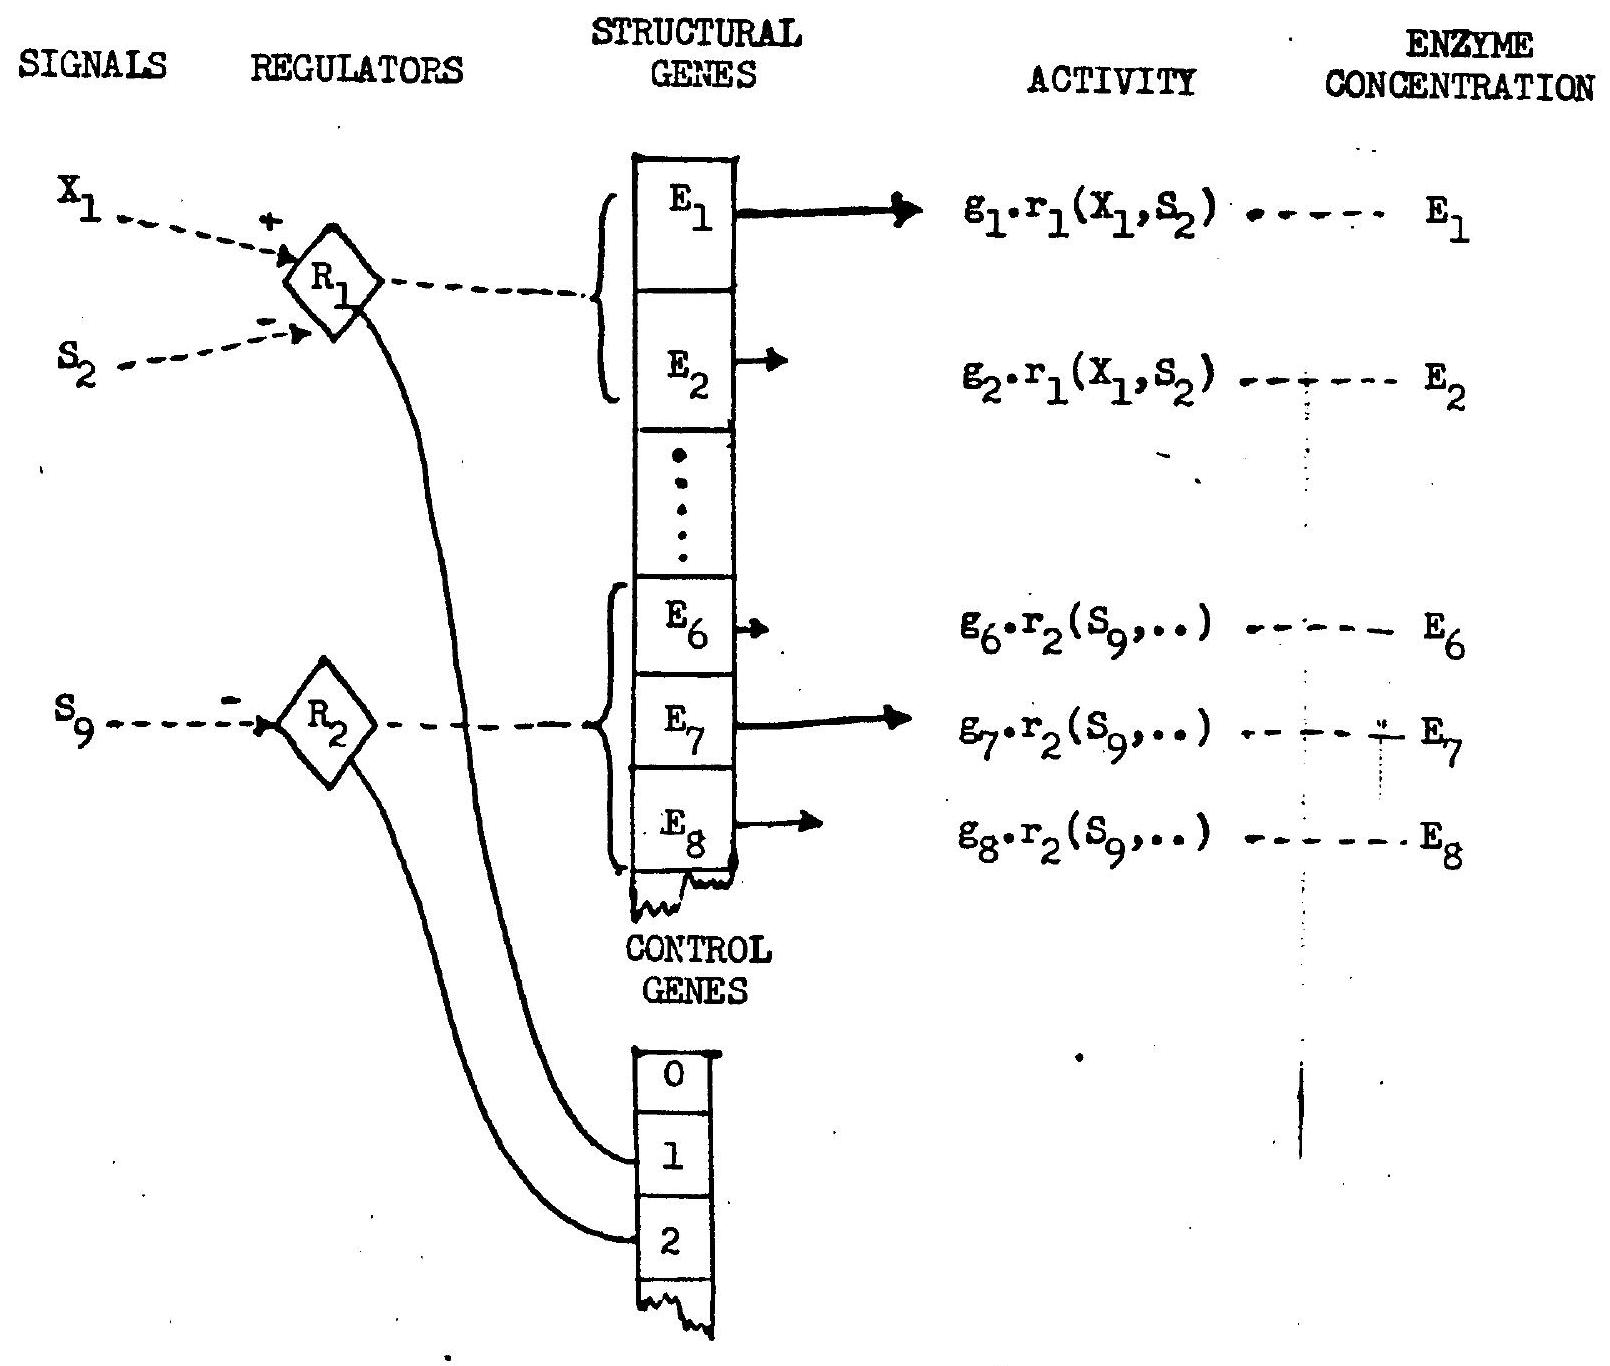
\includegraphics[max width=\textwidth]{2023_01_30_a974a42f7b7381f3f940g-083}
\end{center}

Thus the regulatory protein, represented functionally by say a block of type {(\color{red}Diamond R)} has a `regulatory function', $r_1 (X_1, S_2)$, representing induction by $\mathrm{X}_{1}$ and endogenous repression by $\mathrm{S}_{2}$ and this acts co-ordinately on the enzymes $\mathrm{E}_{1}, \mathrm{E}_{2}$ of the initial pathway. Or again the three enzymes E6, E7, E8 are coordinately repressed by the end product of their pathway, $S_{9}$. Enzymes not subject to control can be formally thought of as under, the control of $R_{0}$ which produces constant gene activity The constants $g_{1}, g_{2}, \ldots$ are determined by the structural genes for enzymes $E_{1}, E_{2}, \ldots$ and are a measure of their intrinsic messenger producing power, thus if two copies of the same structural gene were present its `g' constant would be doubled. The regulatory functions $r_{1}(\ldots)$.. etc. will be represented by suitable algebraic expressions. with values lying between `1' and `0' representing maximum and zero gene activity respectively. Unlike `rate-expressions' there is little theoretical basis for such functions and they are intended only to represent what is known or surmised about the functional aspects of regulation. For example the feedback from $S_{9}$ mediated by the function $r_{2}$ may be of the form $r_{2}\left(S_{9}\right)=1 /\left(1+S_9\right)$, the gene having half of maximal activity at unit concentration of $S_{9}$. More complex functions can express the known features of regulation somewhat better and this will be returned to in $\mathrm{CH}$ IV.

The relation of enzyme concentration to gene activity involves making a number of rather general assumptions and in addition cannot be discussed without involving a `complete' system. However, for the case of a subsystem which can be regarded as a small part of a larger system then the level of an enzyme in the subsystem will be proportional to the activity of its structural gene. Subject then to this restriction that the subsystem is a small part of the whole of metabolism, it becomes possible to consider control loops acting within the subsystem and also from its 'environment', which now includes `constant' internal metabolites, by extending the general equation (2.3) to be
%
\begin{equation}
\varphi_{i}=\sum \lambda_{ij} g_{j} f_{j}(\ldots) \cdot \eta_{jk} {r_{K}}(\ldots)
\label{eqn:29}
\end{equation}
%
Here summation is over $j$ and $k$ and $[\eta{jk}]$ is a regulatory matrix showing which regulator genes control which enzymes. Even when such `control' is added the mathematical situation is unchanged except that an additional type of `block' has to be considered in arriving at the $\varphi_{i}(\ldots$) . The formulation of a system now consists in providing all rate expressions and all regulatory functions together with the stoichiometric and regulatory matrices $\lambda_{ij}$ and $\eta_{jk}$

The introduction of `genotypic parameters', via relation \eqref{eqn:26} , previously assumed, in the diploid case, that enzyme concentration was proportional to gene dosage. If genotypic parameters are embedded in a system with a `control' level this becomes the much more reasonable assumption that 'capacity' for gene action, or the value of g, constants,  is proportional to dosage. If it is further assumed that the alternative alleles at a locus are regulated in parallel, which will often be the case, then (2.9) becomes
%
\begin{equation}
\varphi_{i}(\ldots)=\sum_{j, k} \lambda_{ij}\left[\left(1-\pi_{j}\right) g_{j}^{a} f_{j}^{a}(\cdots)+\pi_{j} g_{j}^{b} f_{j}^{b}(\ldots)\right] \eta_{j  r_{k}}(\ldots)
\label{eqn:210}
\end{equation}
%
\section{Complete growing systems}

On p.58 we considered how to formulate a subsystem within a steadily growing larger system. The effect of growth on pools and fluxes within the subsystem was allowed for by adding an extra flux to expansion' term, $G \times S_i$ away from each pool when formulating the equations for the S.S. The exponential growth constant, $\left.G=\left(\frac{1}{V}\right) {\dot{V}}\right)$, was, in these circumstances, assumed to be given as a fixed parameter. Clearly this is not an adequate formulation if we wish to consider problems such as how the growth constant $G$ itself arises as a system measure and how it is dependant, via the complete system, on the various genetically specified parameters.

The problem of formulating the necessary `complete' systems is theoretically rather different from our previous considerations insofar as it become necessary to specify how the rate of increase of volume, $\dot{v}$, is determined.

Account must also be taken in such systems of the fact that the rate of increase of the different enzymes must compete for the currently available overall synthetic capacity of the system. Thus if more of this capacity is allocated to any enzyme less will be available for all the others. such formulations tend to assume specific mechanisms which are at best of dubious generality. However, a simple type of formulation which represents growth and allows for competition whilst making only fairly general assumptions is as follows.

Let the volume of the system at any instant be $V$ then the rate of change of the total quantity of the ith pool can be expressed in the usual way as

$$\frac{d}{d t}\left(S_{i} \cdot V\right)=\sum \lambda_{ij} \cdot V \cdot E_{j} \cdot f_{j}(S)$$

Suppose that there is some conceptual enzyme $E$, which mediates the overall rate of protein synthesis, representing, perhaps, the complete ribosomal machinery. Assume further that this overall rate (which is responsible for the production of all enzymes) is allocated to a particular enzyme, $E_{j}$, in proportion to priming activity, $g_j$, of its structural genes. On this basis we can write down the rate of increase of the total quantity of the jth protein as follows
%
$$
\frac{d\left(E_{j} V \right)}{dt} =\frac{g_{j}}{\sum g_{j}} \quad V \cdot E_{p} \cdot f_{p}(S)
$$
%
Where the $g_{j}$ may now be functions of pool levels if gene activity is supposed subject to control. Finally suppose that a priming activity, $g_{0}$, decides the allocation to non enzymic structural material such as cell wall. Assuming this structural material to be, synonymous with volume we then have an equation for $\dot{V}$. Thus, where $k$ is a constant, we have
%
$$
\dot{V}=V \times k \times \frac{g_{o}}{\sum g_{j}} \cdot E_{p} \cdot f_{p}(S)
$$
%
Simplifying these equations in the usual way the S.S. of the growing system is defined by
%
\begin{equation}
\begin{aligned}
& \dot{S}_{i}=\sum \lambda_{ij} \olsi{E}_{j} \cdot f_{j}(\olsi{S})-\left(\frac{1}{V} \dot{V}\right) \cdot \olsi{S}_{i}=0  \qquad (a) \\[5pt]
& \dot{E}_{j}=\frac{g_{j}}{\sum g_{j}} \cdot \bar{E}_{p} \cdot f_{p}(S)-\left(\frac{l}{V} \cdot \dot{V}\right) \cdot \olsi{E}_{j}=0 \qquad (b) \\[5pt]
& \left(\frac{1}{V} \dot{V}\right)=\frac{k g_{0}}{\sum g_{j}} \cdot E_{p} \cdot f_{p}(\olsi{S}) \qquad (c)
\end{aligned}
\label{eqn:211}
\end{equation}
%
These can be reduced to only $n$ equations, for the pools $\olsi{S}_{i}$, by using (b) and (c) to eliminate the $\olsi{E}_{j}$ and the term $\left(\frac{l}{\olsi{V}} \dot{V}\right)$ from $(a)$. Thus we have
%
\begin{equation}
\sum \lambda_{ij} g_{j} f_{j}(\olsi{S})-\frac{g_{0}}{\sum g_{j}} \cdot g_{p} \cdot k_{\cdot} f_{p}(\olsi{S}) \cdot S_{i}=0
\label{eqn:212}
\end{equation}
%
Furthermore we can show, from the equation for $\dot{E}_{p}$ in the set $(b)$, that the growth rate, G, is given by a simple measure on the S.S. system defined by \eqref{eqn:212} . Thus
%
\begin{equation}
G=\left(\frac{1}{\olsi{V}} \dot{V}\right)=\frac{g_{p} f_{p}(\olsi{S})}{\sum g_{j}}
\label{eqn:213}
\end{equation}
%
Equations of the type \eqref{eqn:212} are thus suitable for computer studies of the S.S. properties of growing systems with allocation. The question of `optimal allocation' in such systems will be considered at the end of CH. III. 


\chapter{Sensitivity Analysis}

At the start of CH 1 a general mathematical framework was outlined within which it world be possible to consider tho stationary state properties of metabolic systems. Following this, the problem of how any particular system might be formulated in mathematical terms was treated, when it was seen that this necessitated only the provision of a suitable set of rate expressions together with a stoichiometric matrix. Using this formulation it was possible to describe systems ranging from the simple `straight chain of linear unimolecular enzymes' through to complex networks containing bimolecular reactions, enzyme levels modulated by control loops and other non-linear effects.

However, it was pointed out that only for the hypothetical case of a system composed of purely linear reactions was it possible to write down an explicit algebraic solution for the stationary state pools, $\olsi{S}_{i}$, in terms of the genetic and environmental parameters, $P_{1} \ldots, P_{b}$ Even for such linear systems this explicit solution, requiring as it does the inversion of a fixed `D' matrix involved cumbersome algebraic formulae and provided little insight into the way the S.S. is determined by the parameter values. Therefore, since systems of interest tend to possess non-linear features, it appears that even for theoretical `models' we will normally be without any algebraic formulation of the functional relationship connecting the S.S. pools, $\olsi{S}_{i}$, with the parameter values and represented by the following set of equations:
%
\begin{equation}
\olsi{S}_{i}=\olsi{S}_{i}\left(P_{1}, \ldots P_{b}\right), i=1 \text { to } n
\label{eqn:31}
\end{equation}
%
Similarly we will be without the corresponding functions for any measure, $\olsi{M}_{x}$, these functions being represented by the equation below:
%
\begin{equation}
\olsi{M}_{x}=\olsi{M}_{x}\left(P_{1}, \ldots P_{b}\right)
\label{eqn:32}
\end{equation}
%
Given that our main purpose is to `understand' how variation in genetic and environmental parameters will affect properties of the S.S. solution it seems that the `theorist' is reduced to a merely numerical investigation, using a computer to evaluate the functional forms of type \eqref{eqn:31}, \eqref{eqn:32}  for specific values of the parameters.

This places the theorist, using model systems, in a very similar situation to that of the quantitative experimentalist studying real systems, for in each case the basic operation is to modify one or more parameters from some standard position and observe the quantitative effect of this on some system measure(s). The theorist achieves this by using the computer to evaluate this functions (3.2) to any desired accuracy, for a given model and a given set of parameter values, whereas the experimentalist must construct altered genotypes and environments and determine what effect this has on a range of system measures. In both cases, then, data is collected by the procedure of discovering values of the functions \eqref{eqn:32} over some limited region of parameter space. The experimenter and theorist however have different though related aims. The former is usually concerned to establish the structure and parametric values of model metabolic systems witch are consistent with his present data within the limits of experimental accuracy. Hopefully this will enable him to predict the probable outcome of future experiments on his `real', system and at the same time provide a basis for understanding its general quantitative behaviour when subject to parametric disturbances. However, in order to achieve this ho will have to try out a series of models with varying structures and parametric values until a reasonable fit with the data is obtained and such an activity will require considerable general understanding of how the S.S. properties of a system arise out of its structure and parametric values. This leads to a major aim of the quantitative theorist which is to provide a basis for such `understanding' by studying the response to parametric disturbance of a variety of systems of defined structure.

Despite this impossibility of theory to provide simple expressions for functions of type \eqref{eqn:32}, the computer theoretical approach to understanding has distinct advantages over an experimental approach, which attempts to use real systems to achieve the same end. Thus in experimental work the underlying metabolic system, which it is desired to understand, is never known with complete certainty and in addition all measurements and estimates of parameter values are subject to considerable error. Furthermore the effort and time required to construct and measure tho necessary genotype/environment combinations usually limits very severely the number which can be employed when compared with those which can be generated and analysed in a computer study. Thus it can be seen that a study of the response to parameter variation in a variety of model systems can rapidly provide the necessary body of reliable data upon which any understanding of the properties of S.S. systems will have to be based.

A final very considerable advantage of a theoretical study is the possibility of using the computer not only to locate the values, $\olsi{M}$ of relationship \eqref{eqn:32} but also to discover their sensitivity coefficients with respect to one or more of the parameters $P_{1}, P_{2}, \cdots$

This can easily be done for several parameters and measures at a time and, as will be shown in CH IV, involves only a small amount of computation above that already required to merely locate the S.S. The equivalent experimental determinations are, in terms of time and effort, almost impracticable.

\section{Sensitivity coefficients}

Such simulation studies are, of course, purely numerical and can deal only with particular cases. This inherent limitation makes it essential, (Lewontin, 1963), to define clearly what indices of response should be computed and, tentatively, what sort of relations may exist between the various indices descriptive of system response. Only in parallel with such theoretical ideas can the simulation techniques of the next chapter be usefully employed.

In this respect a theoretical index for the response of a measure $\olsi{M}_{x}$ to a differential change in a parameter $P_{y}$ was introduced in the first part of CH.I as $\mathrm{C}_{\mathrm{P}_{\mathrm{y}}^{\mathrm{x}}}^{\olsi{\mathrm{M}}^{\mathrm{x}}}$.

Where
%
\begin{equation}
C_{P_{y}^{X}}^{\olsi{M}}=\frac{P_{y}}{\olsi{M}_{X}} \times \frac{\partial \olsi{M}_{X}}{\partial P_{y}}=P_{y} \dfrac{\partial\left(\log \left(\olsi{M}_{X}\right)\right)}{\partial P_{y}}
\label{eqn:33}
\end{equation}
%
We now wish to explain in more detail the meaning of such sensitivity coefficients and show how a knowledge of their values can aid understanding in both theoretical and real metabolic systems. We will also prove, in a general way, a number of relations between the different coefficients possessed by a system, some of these relations arising out of the `block' structure of metabolic systems while others are merely formal consequences of differential analysis. Clearly, the understanding provided by a knowledge of the sensitivity coefficients will usually be relevant for only a small region of parameter space around an existing steady state, since the coefficients will themselves vary both absolutely and relative to each other when parameters are subject to appreciable change.

\section{Operational meaning of the coefficient}

\stepcounter{equation}
The definition \eqref{eqn:33} gives rise to the approximate relation\footnote{There appears to be no equation (3.4) in the original document.}
%
\begin{equation}
C_{P}^{\olsi{M}} \simeq \frac{\Delta \olsi{M}}{\olsi{M}} \big/ \frac{\Delta P}{P}
\label{eqn:35}
\end{equation}
%
or
%
\begin{equation}
C_{P}^{\olsi{M}} \simeq \frac{\text { fractional response in } \olsi{M}}{\text { small fractional change in P which caused it }}
\label{eqn:36}
\end{equation}

Suppose that a system exists in which it is possible to measure $\olsi{M}$ without error and also to make arbitrarily small changes in a parameter P. To measure $C_P^{\olsi{M}}$ in such a system using the relation \eqref{eqn:36} it is only necessary to create a small disturbance in $P$ and when the system has settled to a new slightly displaced S.S. measure the fractional response in $\olsi{M}$ Thus if a $10 \%$ increase in P produced only a $1 \%$ increase in $\olsi{\mathrm{M}}$ we should have $C_P^{\olsi{M}} \bumpeq 0.1$. Alternatively if the coefficient is known it can be used to estimate the response of $\olsi{M}$ to a small finite change in $P$

Clearly for the limit of increasingly small disturbances tho relation \eqref{eqn:36} defines a measure of response which is independent of the particular units in which $\olsi{M}$ and $P$ happen to be measured and also of the actual size of the disturbance in P. Because of this, the sensitivity coefficient is a more meaningful index of response than, say, the differential coefficient $\frac{\partial \olsi{M}}{\partial P}$.

Knowledge of the relative values of the sensitivity coefficients in a system can give considerable insight into the relative importance of the different variable parameters in controlling different measures. For example the question of which enzyme in a chain of enzymes is 'rate controlling' for the flux through the chain was considered in CH.I to bo equivalent to the question of whether the coefficient of the flux with respect to one of the enzymes was markedly greater than any of the others. Another example arises in relation to a quantitative concept of 'metabolic distance' where we are interested to know whether a disturbance in say, a particular enzyme, E, has a larger effect on pools which are situated close to it on the metabolic chart than on pools which appear to be more distant. In this case the relative values of the coefficient $C_{E}^{S_1}, C_{E}^{S_2}, \ldots$, would enable us to see whether `chart' distance, perhaps measured as the number of intervening metabolic steps, is generally similar to quantitative `metabolic distance'.

The two examples just given show that it would be of little use to know a single coefficient since usually we are interested in comparisons between a group of coefficients, either over different measures or with respect to different parameters. In general, therefore, it is valuable to know a matrix of coefficients $\left[\olsi{C}^{\olsi{M}}_{P_y}\right]$ whore $x$ an $y$ run over a suitable set of measures and parameters respectively. It was mentioned previously that such a matrix can ba obtained automatically almost as a by-product of this computation necessary to evaluate the set of function \eqref{eqn:32}, and it is therefore advantageous in computer studies to obtain this matrix since it provides a great deal of extra information about this response of the system to parameter variation. In real systems, however, considerable effort is necessary to measure each coefficient and it will usually not be possible or worthwhile to build up any sort of matrix by straightforward measurements. However, in many systems the measurement of the response of pools and independent fluxes to only a few parameter modulations together with a knowledge of the ratios of the independent fluxes will enable the relative values of many coefficients of interest to be found without excessive experimental effort. This can be done by using our prion knowledge of the `structure' of system and employing the methods and relationships set forth later in this chapter.

\section{Formal relations of different measures}

Although at first sight it appears that there are as many independent measurements on the S.S. of a system as one cares to make; it will in fact often happen that a measure is related in some way to other measures.

For example it was pointed out on p.52 that in a system with m transformational steps and n pools it is always possible to express $n$ of the S.S. fluxes as linear combinations of remaining $(m-n)$. A simple illustration of this is a divided pathway where the flux, F, in the main chain mast be equal to the sum of the fluxes $\left(F_{1}, F_{2}\right)$ in the separate arms or
%
\begin{equation}
F = F_{1}+F_{2}
\label{eqn:37}
\end{equation}
%
A general formal result will now be obtained for use whenever such dependance between measures exists. Suppose that a measure $\olsi{M}$ depends in some way on a set of other measures $\olsi{M}_{1}, \olsi{M}_{2}, \ldots$ and possibly directly on various parameters of type $P$, this can be expressed in the usual functional notation by
%
\begin{equation}
\olsi{M} = \olsi{M}\left(\olsi{M}_{1}\left(P_{1}, \ldots\right), \olsi{M}_{2}(\ldots), \ldots, P_{d}, P_{e}\right)
\label{eqn:38}
\end{equation}
%
Where each of the measures $\olsi{M}_{1}, \olsi{M}_{2}, \ldots$ is itself regarded as a function of the system parameters. By applying the formal rules of partial differentiation to (3.8) we obtain, with respect to $P_{k}$
%
$$
C_{P_k}^{\olsi{M}}=\frac{P_k}{\olsi{M}} \frac{\partial \olsi{M}}{\partial P_k}=\frac{P_k}{\olsi{M}}\left[\frac{\partial \olsi{M}}{\partial P_k}\right] + \sum \frac{M_i}{\olsi{M}}\left[\frac{\partial \olsi{M}}{\partial \olsi{M}_i}\right] \cdot \frac{P_k}{\olsi{M}_i} \frac{\partial M_i}{\partial P_k} $$
%
or
\begin{equation}
\quad C_{P_{k}}^{\olsi{M}}=\left[C_{P_{k}}^{\olsi{M}}\right]+ \sum C_{P_{k}}^{\olsi{M}_{i}} \left[C^{\olsi{M}}_{M_i}\right]
\label{eqn:39}
\end{equation}
%
In this formula the coefficients enclosed within square brackets refer to tho sensitivity of function \eqref{eqn:38} considered in isolation from the overall system, whereas the ordinary system coefficients are, unbracketted. Iwo examples will be given to illustrate what is meant by this:

A) Taking the simple branched pathway case of \eqref{eqn:37} we have
%
$$
\left[C_{F_{1}}^{F_{1}}\right] = \frac{F_{1}}{F} \frac{\partial\left(F_{1}+F_{2}\right)}{\partial F_{1}}=\frac{F_{1}}{F_{1}+F_{2}}
$$
%
and similarly $\left[\mathrm{C}_{\mathrm{F}_{2}}^{\mathrm{F}}\right]=\frac{\mathrm{F}}{\mathrm{F}_{1}+\mathrm{F}_{2}} \cdot$ Then, since no parameter is directly involved in \eqref{eqn:37} the general relation \eqref{eqn:39} gives:
%
\begin{equation}
C_{P}^{F}=\frac{F_{1}}{F_{1}+F_{2}} \cdot C_{P}^{F_{1}}+\frac{F_{2}}{F_{1}+F_{2}} \cdot C_{P}^{F_{2}}
\label{eqn:310}
\end{equation}
%
This shows that the sensitivity of the main flux to any parameter is just a weighted sum of the sensitivity of the pathway fluxes; the weighting being proportional to the contribution of each branch to the main flux.

B) A simpler form of the relation \eqref{eqn:37} occurs when a measure $\olsi{M}$ results from multiplying and dividing together a set of other measures. Consider for example
%
$$
\begin{aligned}
\olsi{\mathrm{M}}=\left(\olsi{M}_{1} \times \olsi{M}_{2}\right) /\left(\olsi{M}_{3} \times \olsi{M}_{4}\right), \\[4pt]
\text { In this case } C^{M}){\olsi{M}_1} = 1 \text { and similarly for } \olsi{M}_{2} \text {, } \\
\text { also } C^{\olsi{M}}_{\olsi{M}_3} = -1 \text {, and similarly for } \olsi{M}_{4} \text {, So that \eqref{eqn:39} } \\
\end{aligned}
$$
becomes
%
\begin{equation}
C_{P}^{\olsi{M}} = C_{P}^{M_1} + C_{P}^{M_{2}} - C_{P}^{M_{3}}- C_{P}^{M_{4}}
\label{eqn:311}
\end{equation}
%
Thus when a measure is formed by multiplication and division of a set of measures its coefficient with respect to any parameter is merely the sum of the separate coefficients of the measures in the numerator minus that of the measures in the denominator.

\section{Block coefficients}

In the last chapter it was shown that metabolic systems can be regarded as made up of functional blocks. Thus `transformational blocks' which could be enzymic or non enzymic, were represented in a diagram by,

\centerline{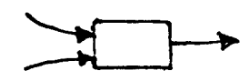
\includegraphics[scale=0.7]{figure3_block.png}}

described by a rate expression giving, $F$, the net flux carried by the block. Similarly there were `regulatory blocks' represented by, \scalebox{2}{$\diamond$} and quantitatively described by a regulatory function, $R$, giving the fraction by which the maximal activity of a structural locus should be multiplied to take account of regulation.

The concept of the sensitivity coefficient $C_{P}^{M}$ was introduced as a means to describing and measuring the nett effect of changes in genetically determined parameters on some systemic property say the measure $\olsi{M}$. Even with the simplest rate expression, a number of parameters are associated with each block and this number increases considerably when bimolecularity, regulation and inhibition has to be introduced. Insofar as all such parametric changes can affect the system only by acting through the one block, it is convenient to consider their common effect by defining a new coefficient, the `block coefficient'. It will be shown that, on the other hand, the differences between the effects of parameter within a given block are described by a set of further coefficients descriptive of the behaviour of the isolated block.

The block coefficient is introduced by the following considerations. A fairly general set of equations defining the S.S. was of the form
%
\begin{equation}
\sum \lambda_{i \mathbf{j}} F_{\mathfrak{j}}=0
\label{eqn:312}
\end{equation}
%
Where $F_{j}$ stands for a 'complete' transformational expression involving, in general, both a rate expression $f_{j}$ and a regulatory function $R_{k}$.

Consider a new `constructed' system related to the original one in that each complete transformational expression, in (3.32), is replaced by a modified form $F^{\prime}_j$ obtained by multiplying each $F$ in \eqref{eqn:312}  by an extra parameter $\alpha_{j}$. When the constructed system has all its $\alpha_{j}$ equal to unity it will, of course, have the same S.S. solution as the original system and will behave identically with regard to other parameter variations. The equations defining the S.S. of the constructed system will be
%
\begin{equation}
\sum \lambda_{ij} \alpha_{j} F_{j}=0
\label{eqn:313}
\end{equation}
%
The coefficient of a measure $\olsi{M}$ with respect to, say, the 3rd transformational block in the constructed system can now be defined in the usual way as
%
\begin{equation}
C_{\alpha_{3}}^{\olsi{M}}=\frac{\alpha_{3}}{\olsi{M}} \cdot \frac{\partial \olsi{M}}{\partial a_{3}}
\label{eqn:314}
\end{equation}
%
The block coefficient in the original system is then defined as $C^{\olsi{M}}_{\alpha_3}$ evaluated with all $\alpha$'s equal to unity, that is around the position where the original and the constructed systems behave identically.

It will now be shown how the sensitivity coefficient, $C_{P}^{\olsi{M}}$, is related to $\mathrm{C}_{\alpha_{3}}^{\olsi{M}}$ when $P$ is a parameter embedded within the expression $F_{3}$.

The relation can be discovered by considering that it is always possible to make simultaneous small changes $\Delta \alpha_{3}$ and $\Delta \mathrm{P}$ such that the S.S. solution, $\olsi{S}_{i}$, will remain completely unchanged, as also will all measures on this S.S. not directly involving $\alpha_{3}$ or $P$. This gives rise to two relations.

Considering first, the system as a whole it gives rise to the relation
%
\begin{equation}
C_{\alpha_{3}}^{\olsi{M}} \cdot \frac{\Delta \alpha_{3}}{\alpha_{3}} + C_{P}^{M} \cdot \frac{\Delta P}{P} = 0 \tag{a}
\label{eqn:315a}
\end{equation}
%
On the other hand considering the transformational flux expression, $F_{3}^{\prime}$, in isolation, and noting that the only quantities occurring in it which are subject to change are $\alpha_{3}$ and $P$ and that these produce zero net effect we have
%
\begin{equation}
\left[\mathrm{C}_{\alpha_{3}}^{\mathrm{F}_{3}^{\prime}}\right] \cdot \frac{\Delta \alpha_{3}}{\alpha_{3}} + \left[\mathrm{C}_{\mathrm{P}}^{\mathrm{F}^{\prime}_3}\right] \cdot \frac{\Delta \mathrm{P}}{\mathrm{P}}=0 \tag{b}
\label{eqn:315b}
\end{equation}
%
in (b) the square brackets are used to denote coefficients of the transformational flux expression, considered in isolation from the and rest of the system and with respect to one of its arguments.

Combining (a) and (b) and remembering that, since $\mathrm{F}_{3}^{\prime}=\alpha_{3} \cdot \mathrm{F}_{3^{\prime}}$
%
$$
\left[C^{F^{\prime}}_{\alpha_3}\right]=1 \text { and }\left[C_{P}^{F^{\prime}}\right] \equiv\left[C_{P}^{F}\right] \text { we get }
$$
%
\begin{equation}
C_{P}^{\olsi{M}} = C_{\alpha_3}^{\olsi{M}} \cdot\left[C_{P}^{F_{3}}\right]
\label{eqn:315}
\end{equation}
%
The relationship \eqref{eqn:315} which applies in both the original and the constructed system, states that the sensitivity of a measure $\olsi{M}$ to a parameter $P$ will depend jointly on the sensitivity of $\olsi{M}$ to the block in which $P$ acts and on the sensitivity of the flux through this block, when considered in isolation from the rest of the system, to the parameter $P$ itself.

In the more general case where the parameter $P$ occurs in connection with several transformational blocks (such as multiple inhibition by an external. substance) the relation \eqref{eqn:315} becomes
%
\begin{equation}
C_{P}^{\olsi{M}}=\sum C_{\alpha_{r}}^{\olsi{M}} \times \left[C_{P}^{F_r}\right]
\label{eqn:316}
\end{equation}
%
where the summation effectively extends over all blocks influenced directly by P. Consider for example a system, as indicated below, containing a group of three enzymes having rate expressions $f_{1}, f_{2}, f_{3}$ and each under co-ordinate control from a block with regulatory function $\mathrm{R_1}$

\begin{center}
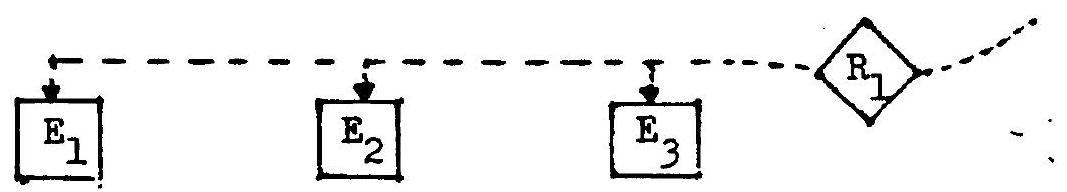
\includegraphics[max width=\textwidth]{2023_01_30_a974a42f7b7381f3f940g-101}
\end{center}

The separate $f$ flux expressions will then be $f_{1} \times R_{1}, f_{2} \times R_{1}, f_{3} \times R_{1}$, and the sensitivity of any measure $\olsi{M}$ to the regulatory block, $R_{1}$, can be considered as the sensitivity to a parameter $\beta$, of value unity, multiplying into the regulatory function $\mathrm{R}_{1} \cdot$ Using the relation \eqref{eqn:316} we get
%
$$
C_{\beta}^{\olsi{M}} = C_{\alpha_{1}}^{\olsi{M}_{1}} \cdot \left[C_{\beta}^{f_{1} \times \beta \times R_1}\right] + C_{\alpha_{2}}^{M}\left[C_{\beta}^{f_{2} \times \beta \times R_1} \right]+\cdots
$$
%
Using the formal relationship \eqref{eqn:311}  to simplify the bracketed expressions we get
%
$$
C_{\beta}^{M} = C_{\alpha_{1}}^{M} + C_{\alpha_{2}}^{M} + C_{\alpha_{3}}^{M}.
$$
%
This result shows that the sensitivity to the regulatory block is just the sum of the sensitivities to the separate transformational blocks involved in the co-ordinate regulation.

\subsection{Coefficient with respect to an enzyme}

In a system where enzyme quantities are specified as parameters, that is one in which no gene control loops are operative, all flux expressions will be of the form
%
\begin{equation}
F_{j}=E_{j} \times f_{j}(--)
\label{eqn:317}
\end{equation}
%
Using, relation \eqref{eqn:315}  to connect the block coefficient to the enzyme we have
%
$$
C_{E_j}^{M}= C_{\alpha_{j}}^{M} \cdot\left[{C_{E}^{F_j}}\right]
$$
%
then using \eqref{eqn:317} and the formal relationship \eqref{eqn:311}
%
$$
C_{E_j}^{M} = C_{\alpha_j}^{M} \left[ C_{E_j}^{E^j} \right] + \left[ C^{f_j}_{E_j}\right] = C_{\alpha_{j}}^{M}(1+0)
$$
%
so that
%
\begin{equation}
C^M_{E_j} \equiv C^M_{\alpha_j}
\label{eqn:318}
\end{equation}

Thus for such a system, the block coefficient is synonymous with the coefficient with respect to enzyme quantity previously considered in CH. 1. When, however, the enzyme level is subject to control there is no such identity since $E_{j}$ is no longer a parameter and $C_{E_{j}}^{M}$ has no clear meaning.

\subsection{Coefficient with respect to turnover number}

Even when enzyme quantity is subject to control, the rate expression will still be of the form $F_{j}=E_{j} (\cdots) t_{j} f_{j} (\cdots)$ Where the enzyme level, $E_{j}$, is now a function of some sort and $t_{j}$ is the turnover number. In this case an argument, similar to that above, will show that
%
\begin{equation}
C_{\alpha_{j}}^{M} \equiv C_{t_{j}}^{M}
\label{eqn:319}
\end{equation}
%

\subsection{Coefficient with respect to gene dosage}

When control is operative and on the assumption that the system under consideration is a small part of some larger system the gene dosage parameter $g_{j}$ introduced in the last chapter will always appear multiplied into the complete flux expression for the jth transformation or
%
$$
F_{j}=g_{j} \times t_{j} \times f_{j}(-) \times n_{jk} \times R_{k}(-)
$$
%
Therefore once again
%
\begin{equation}
\mathrm{C}_{\alpha_j}^{\olsi{M}} \equiv \mathrm{C}_{g_j}^{\olsi{M}}.
\label{eqn:320}
\end{equation}
%
A slight correction to this result will be necessary if it is conceded that the system under consideration is not a small part of a larger system but it will still be approximately true. Another difficulty arises, in relation to the meaning of $\mathrm{C}_{g_{j}}^{M}$ in (3.2.0), because in most organisms it is not possible to vary $g_{j}$ continuously. However, this problem will not arise in e.g. Neurospora where $g_{j}$ can be varied almost continuously

\section{Measurement of coefficients in a `real' system}

From the foregoing it can be seen that in understanding a real system considerable insight will be obtained if the sensitivity of a selected set of measures can be determined even with respect to each transformational block, rather than for all parameters. These block coefficients cannot usually be measured as $C_{E}^{\olsi{M}}$ since in most systems there is some degree of enzyme control and enzyme quantity is not a true parameter. However, there is no such objection to obtaining the block coefficients via $C_{t_j}^{\olsi{M}}$ or $C_{g_{j}}^{\olsi{M}}$ and both of these methods have been employed. Even so several difficulties arise in practice. Thus, since it is not easy, to measure small changes in $\olsi{M}$ and $P$ with sufficient accuracy, it will usually be necessary to measure $\olsi{M}$ as accurately as possible for a number of more widely spaced `P' values and construct a smooth curve showing the relationship between $\olsi{M}$ and $P$ when all other parameters are held constant. From this curve $C_{P}^{\olsi{M}}$ can be estimated around the original $P$ value using the definition (3.6). When the sensitivity with respect to external concentration (of type $X$) is required no further difficulties arise since such quantities can be varied continuously and measured with reasonable accuracy. However, in order to measure internal `block' coefficients it is necessary to produce a controlled change in a single internal (genetically controlled) parameter and this is not always simple, or indeed possible.

For example, one way of estimating the block coefficient of an enzyme would be to measure $C_{t}^{M}$ using a series of revertants from a mutant in which the activity of the enzyme had been abolished by a mutation at its structural locus. Unfortunately each of these `new' proteins would not only have a different turnover number from the original enzyme but, in general, also different values for all the other kinetic parameters characterising the protein. In such a case it is only possible to plot $\olsi{M}$ against turnover number after establishing that other kinetic parameters are effectively uncharged. A method of this general type has been employed by C. Chilcott (Honours Thesis, Edinburgh, 1961) and B. I. Barthelmess (personal communication) using revertants in the arginine pathway of N.crassa. Another method, which is intended to avoid the complication of simultaneous changes occurring in several parameters, is to attempt to alter only the quantity of a particular structural gene. In principle this can be done by altering the `dose', that is the parameter $g_{j \text { ' }}$ and estimating the block coefficient via $\mathrm{C}_{\mathrm{g}_{j}}^{\mathrm{M}}$.

A way in which a particular $g_{j}$ can be altered almost continuously without altering anything else is by constructing heterokaryons in fungi between wild type and a strain in which activity at the structural locus in question is abolished. By varying the input of the two types contributing to the heterokaryon the dosage of the structural gene in question can be controlled over a considerable range. A method of this general type has been employed by W. Tateson (Ph.D. Thesis, Edinburgh, 1971), also for steps in the arginine pathway of Neurospora.

Since it is clear that the determination of coefficients by these `direct' experiments is extremely laborious, it is important, to establish any further general properties of coefficients, particularly in relation to the expected distribution of control between different blocks and to any 'diagnostics' which would make it easier to determine the pattern of coefficients experimentally. We will return to this subject after considering the various relations between coefficients and demonstrating how the coefficient values arise from measurable properties of the individual transformation blocks.

\section{Summation properties of block coefficients}

At the end of CH.I it was shown, relation (1.31), that the sum of the flux-control coefficients in a chain of non linear enzymes was equal to unity. Now that we have suitably extended the definition of
coefficient to general networks and networks in which enzyme quantities cannot be treated as a parameter it will be demonstrated that this and other properties still hold, being indeed a very general and simple consequence of the block structure of metabolic systems.

Thus consider the general S.S. equations (3.13) defining the constructed system:

$$
\sum \lambda_{ij} \alpha_j F_j = 0
$$

I. ``The sum of the sensitivity coefficients of any given pool, $S$, with respect to each of the separate transformation blocks in the system is zero''

\tcbset{colback=yellow!10!white, colframe=red!50!black,leftrule=0.45mm,
        highlight math style= {enhanced, %<-- needed for the ’remember’ options
            colframe=red,colback=red!10!white,boxsep=0pt}
        }

\begin{tcolorbox}[ams equation]
\sum_{j=1, \ldots m} C_{\alpha_j}^{\olsi{S}}=0
\label{eqn:321}
\end{tcolorbox}


II. ``The sum of the sensitivity coefficients of any given flux, $F$, in the system with respect to each of the separate transformation blocks in the system is unity''

\begin{tcolorbox}[ams equation]
\sum_{j=1, \ldots m} C_{\alpha_j}^{\olsi{F}} = 1
\label{eqn:322}
\end{tcolorbox}

These two results can be obtained by supposing that the same fractional differential change $x$ is made in all the $\alpha_{j}$. Then for a given pool the fractional response is found by summing up the responses predicted from the separate sensitivities or:
%
$$
\frac{\Delta S}{S}= \sum C_{\alpha_{j}}^{S} \cdot x
$$
%
But $\frac{\Delta S}{S}=0$, from the co-ordinate property. Therefore $\sum \mathrm{C}_{\alpha_{j}}^{\mathrm{S}}=0$, as required.

In the case of the flux coefficients we have, similarly.

$$
\frac{\Delta F}{F} = \sum C_{\alpha_{j}}^{F} \cdot x
$$
%
and in this case the co-ordinate property predicts $\frac{\Delta \mathrm{F}}{F}=\mathrm{x}$, so that
%
$$
x = \sum \mathrm{C}_{\alpha_{\mathbf{j}}}^{F} \cdot x \text { or } \sum \mathrm{C}_{\alpha_{\mathbf{j}}}^{F}=1 \text {, as required }
$$
%
The result (3.22) is particularly useful in relation to the problem of discovering the rate-controlling enzyme for a particular flux in an experimental situation. Thus it predicts that provided that, the structure is such that all coefficients are +ve, the value of the coefficient for a rate controlling enzyme would have to be close to unity. This means that a single experiment on a suspected enzyme can confirm or deny the hypothesis that it is the rate controlling one. Whereas in the absence of an expected value for the coefficient of a rate-controlling enzyme it would be necessary to perform such an experiment for all the enzymes in the system and compare their values, which is hardly practical.. Unfortunately no simple prediction can be made when -ve coefficients are a possibility, as for example in systems having divided pathways.

The result (3.21) for pool coefficients shows that they must be both +ve and -ve but otherwise places no limit on their values. In a later section it will be shown, by algebraic study of a simples system, that there is no general restriction on the values which can be taken by the individual coefficients of either pools or fluxes.

\section{Elasticities of complete flux expressions}

In the preceding discussion of block coefficients the sensitivity of a complete flux expression, $F_{j}$, in isolation from the rest of the system was used, that is for one of its arguments when all others are held at their S.S. levels. This was expressed by enclosing the ordinary sensitivity coefficient notation in square brackets as for example $\left[C_{P}^{F_r}\right]$ in (3.16). Such terms occur frequently in relations between system block coefficients and it is useful to distinguish them from these by a suitable notation. Accordingly we call them `elasticities' writing the above example as $\varepsilon_{p}^{F_r}$.
%
\begin{equation}
C_{P}^{\olsi{M}} = \sum C_{\alpha_{r}}^{\olsi{M}} \cdot \varepsilon^{F_r}_P
\label{eqn:323}
\end{equation}
%
The elasticities of a flux expression are, of course, not constant but will depend on the operating conditions of the appropriate enzymes under in vivo S.S. conditions. In principle they could be measured by extracting the appropriate enzymes, reconstructing their exact operating conditions in vitro and determining the sensitivity of the flux to separate modulations in substrates, products, regulators etc. In practice such a procedure is not usually feasible but it will be shown later in this chapter that it is still possible to obtain estimates of all elasticities by considering data from modulation experiments carried out around an existing S.S. in vivo.

Using the idea of elasticity it becomes straightforward to write down the response of a typical flux expression, considered in isolation, to variation in it's arguments. Thus consider the subunits indicated below which together define the flux expression $F_{1}$

\begin{center}
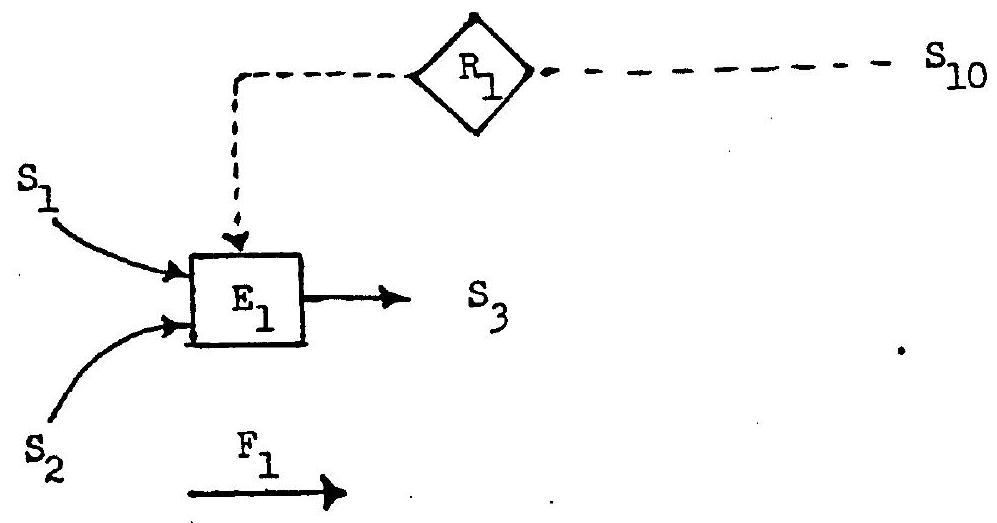
\includegraphics[max width=0.6\textwidth]{2023_01_30_a974a42f7b7381f3f940g-110}
\end{center}

If $\alpha_{1}$ is modulated it will produce consequent changes in $S_{1}, S_{2}, F_{1}$ and throughout the system, but it will. always be true that:
%
$$
\frac{\Delta F_{1}}{F_{1}} = \varepsilon^{F_1}_{\alpha_{1}} \cdot \frac{\Delta \alpha_{1}}{\alpha_{1}} + \varepsilon^{F_{1}}_{S_{1}} \cdot \frac{\Delta S_{1}}{S_{1}} + \varepsilon_{S_{2}}^{F_{1}} \cdot \frac{\Delta S_{2}}{S_{2}} + \ldots
$$
%
Here the complete flux expression $F_{1}$ involves more than just the rate equation, being of the form:
%
$$
F_{1}=\alpha_{1} \cdot f_{1}\left(S_{1}, S_{2}, S_{3}\right) \cdot R\left(S_{10}\right)
$$
%
Consequently the elasticities can be simplified, for example
%
$$
\varepsilon_{\alpha_{1}}^{F_{1}} = 1
$$
%
$$
\varepsilon_{S_{1}}^{F_{1}} = \varepsilon_{S_{1}}^{f_{1}}
$$
%
and $\quad \varepsilon_{S_{10}}^{F_{1}}=\quad \varepsilon^{R_{1}}_{S_{10}}$. So that
%
$$
\frac{\Delta F_{1}}{F_{1}}=\frac{\Delta \alpha_{1}}{a_{1}}+ \varepsilon_{S_{1}}^{f_{1}} \cdot \frac{\Delta S_{1}}{S_{1}} + \varepsilon_{S_{2}}^{f_{1}} \cdot \frac{\Delta S_{2}}{S_{2}}+ \varepsilon_{S_{3}}^{f_2} \cdot \frac{\Delta S_{3}}{S_{2}}+ \varepsilon_{S_{10}}^{R} \frac{\Delta S_{10}}{S_{10}}
$$

Expressions of this type will be used in subsequent discussion.

\section{Relative Importance of two successive enzymes in a straight chain}

The situation often arises, even within a complex system, that two enzymes can be found such that the product of one is the substrate of the next and has no strong interaction with any other protein in the system. Such a situation is indicate below for two hypothetical enzymes, $\mathrm{E}_{1}$ and $E_{2}$, which may be quite complicated such as being bimolecular and suffering inhibition.

\begin{center}
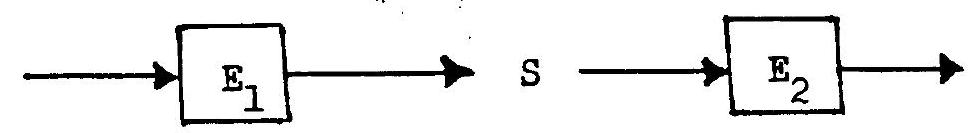
\includegraphics[max width=0.6\textwidth]{2023_01_30_a974a42f7b7381f3f940g-112}
\end{center}

Provided that $S$ only affects $E_{1}$ and $E_{2}$ it will always be possible to make simultaneous changes in the block parameters $\alpha_{1}, \alpha_{2}$ such that only $S$ is altered. This is achieved by increasing $\alpha_{1}$ and then decreasing $\alpha_{2}$ so as to exactly cancel the effect on all pools and fluxes other than the common pool S. Suppose that such an operation produces a small fractional change $\frac{\Delta S}{S}$ in S. Considering the flux expression, $F_{1}$, in isolation from the rest of the system and noting that simultaneous changes in $\alpha_{1}$ and $S$ produce no change in $F_{1}$, we have, using the elasticity notation
%
$$
\varepsilon_{\alpha_{1}}^{F_{1}} \cdot \frac{\Delta{ }^{\alpha_1}}{\alpha_1} + \varepsilon_S^{F_1} \cdot \frac{\Delta \mathrm{S}}{\mathrm{S}}=0
$$
%
or
%
\begin{equation}
\quad \frac{\Delta \alpha_{1}}{\alpha_{1}} = -\varepsilon_{S}^{F_1} \cdot \frac{\Delta S}{S} \tag{a}
\label{eqn:323a}
\end{equation}
%
Similarly for $E_2$
\begin{equation}
\frac{\Delta \alpha_2}{\alpha_2}=-\varepsilon_S^{F_2} \cdot \frac{\Delta S}{S} \tag{b}
\label{eqn:323b}
\end{equation}

Finally, since the simultaneous changes in $\alpha_{1}, \alpha_{2}$ have no effect on any system measure, except $S$, we have for the whole system,
%
\begin{equation}
C_{\alpha_{1}}^{M} \cdot \frac{\Delta \alpha_{1}}{\alpha_{1}}+C_{\alpha_{2}}^{M} \cdot \frac{\Delta \alpha_{2}}{a_{2}}=0 \tag{c}
\label{eqn:323c}
\end{equation}
%
where $C_{\alpha}^{M}$ are the ordinary systemic block coefficients of a measure M.

Combining the three equations $a, b, c$, we have that for two successive enzymes in a chain the ratio of their sensitivity coefficients $C_{1}, C_{2}$ for any measure is given by

\begin{tcolorbox}[ams equation]
\frac{C_1}{C_2} = -\frac{\varepsilon^{F_2}_2}{\varepsilon^{F_1}_1}
\label{eqn:324}
\end{tcolorbox}

This result will be true no matter how complex the system within which the two enzymes are embedded.

For example consider two `linear' enzymes, $E_{1}$ and $E_{2}$ within some larger system as indicated below and suppose them subject to repression via a manression function $R$ and the first one to non competitive inhibition with an inhibitory function $\phi$.

\begin{center}
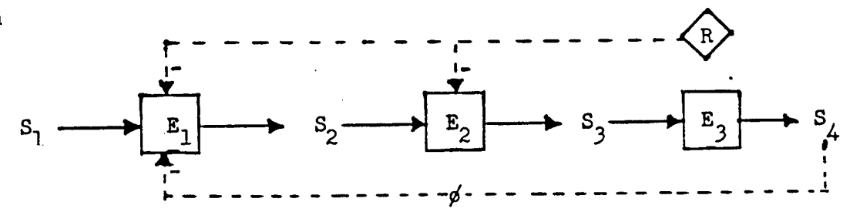
\includegraphics[max width=\textwidth]{figure3_324.png}
\end{center}

To find the relative importance of their block coefficients for a.1 measures (other than $S_2$) we apply $\left(3.24\right)$ or
%
$$ \frac{C_1}{C_2} = -\frac{\varepsilon_{S_2}^{F_2}}{\varepsilon_{S_2}^{F_1}} = -\frac{\varepsilon_{S_2}^{\left(\alpha_2 \cdot f_2 \cdot R\right)}}{\varepsilon_{S_2}^{\left(\alpha_1 \cdot f_1 \cdot R \cdot \phi\right)}} $$
%
Using the formal relation (3.11) to simplify this we get
%
$$
\frac{C_{1}}{C_{2}}=\frac{\varepsilon_{S_{2}}^{\alpha_{2}}+\varepsilon_{S_{2}}^{f_{2}}+\varepsilon_{S_{2}}^{R}}{\varepsilon_{S_{2}}^{a_{1}}+\varepsilon_{S_{2}}^{f_{1}}+\varepsilon_{S_{2}}^{R}+\varepsilon^\phi_{S_{2}}} = \frac{0+\varepsilon_{S_{2}}^{f_{2}}+0}{0+\varepsilon_{S_{2}}^{f_{1}}+0+0}
$$
%
or
%
$$\quad \frac{C_{1}}{C_{2}}=\frac{\varepsilon_{S_{2}}^{f_{2}}}{\varepsilon_{S_{1}}^{f_{2}}}$$
%
so that the ratio of block coefficients depends on the ratio of the elasticities of the two rate expressions with respect to the common pool. In particular, if the reactions are linear, $f_{1}$ will be of the form
%
$$ f_{1}= v_{1}\left(S_{1}-\frac{S_{2}}{K_{1}}\right)$$,
%
and using the definition (3.3) for the coefficient we have
%
$$
\varepsilon_\mathrm{S_2}^{f_1} = \left[\mathrm{C}^{\mathrm{f}_{1}}_{\mathrm{S}_{2}}\right] = \mathrm{S_2} \frac{\partial\left(\log \mathrm{f}_{1}\right)}{d\mathrm{S}_{2}}=\frac{\mathrm{S}_{2} / \mathrm{K}_{1}}{\mathrm{S}_{1}-\mathrm{S}_{2} / \mathrm{K}_{1}}
$$
%
$$
\begin{aligned}
& \text { similarly } \quad \varepsilon^{f_2}_{S_2} = \frac{\mathrm{S}_{2}}{\mathrm{S}_{2} - \mathrm{S}_{3} / \mathrm{K}_{2}} \\[5pt]
& \text { so that } \quad \frac{\mathrm{C}_{1}}{\mathrm{C}_{2}}=\frac{\left(\mathrm{S}_{1}-\mathrm{S}_{2} / \mathrm{K}_{1}\right)}{\left(\mathrm{S}_{2}-\mathrm{S}_{3} / \mathrm{K}_{2}\right)} \cdot \mathrm{K}_{1}
\end{aligned}
$$
%
The two terms in numerator and denominator will be recognised as the `out-of-equilibrium' of the two steps. This confirms and extends the result in CH.I concerning the usefulness of the `out-of-equilibrium' term as a diagnostic for rate control in simple cases.

\section{Relation between the coefficients of all blocks affected a given pool}

The relation (3.24) applying to two successive blocks affected by a common pool can now be generalised to cases where the given pool influences more than two enzymes, as for example if it is a signal for repression or perhaps at the dividing point of a branched pathway.

Since it turns out that the argument does not depend on the \underline{flux} relationship of the influenced enzymes it will be sufficient to refer to a general pool influence diagram, indicated below for enzymes $\mathrm{E}_{1}, \mathrm{E}_{2}, \mathrm{E}_{3}$ and $E_{4}$ which are all affected by pool S. In this diagram the dotted lines signify influence, that is non zero elasticities with respect to $S$, and flux arrows, which may coincide, have been omitted.

\begin{center}
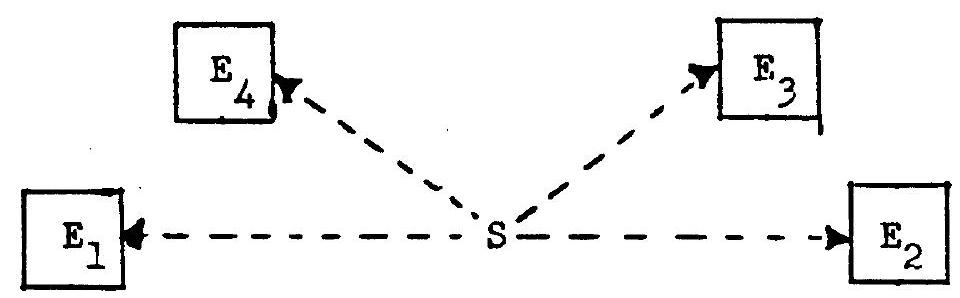
\includegraphics[max width=0.8\textwidth]{2023_01_30_a974a42f7b7381f3f940g-115}
\end{center}

As in the previous argument, when S affected only two enzymes, it is always possible to make simultaneous movements in $\alpha_{1}, \alpha_{2}, \alpha_{3}$ and $\alpha_{4}$ such that only $S$ is changed, all other pools in the system remaining constant. By considering $F_{1}$ in isolation we must have:
%
$$ 0 = \frac{\Delta F_1}{F_1} = \varepsilon_{\alpha_1}^{F_1} \cdot \frac{\Delta \alpha_1}{\alpha_1}+ \varepsilon^{F_1}_S \cdot \frac{\Delta_S}{S} $$
%
or
%
\begin{equation}
\frac{\Delta \alpha_{1}}{\alpha_{1}}=\varepsilon_{S}^{F_1} \cdot \frac{\Delta S}{S} \tag{a}
\label{eqn:324a}
\end{equation}
%
and similar relationships for $\mathrm{E}_{2}, \mathrm{E}_{3}$ and $\mathrm{E}_{4}$

Also since no measure, other than $S$, is affected by these simultaneous changes in the a values, we can write for the system as a whole
%
\begin{equation}
C_{\alpha_{1}}^{M} \cdot \frac{\Delta \alpha_{1}}{\alpha_{1}}+ C_{\alpha_{2}}^{M} \cdot \frac{\Delta \alpha_{2}}{\alpha_{2}} + \ldots =0 \tag{b}
\label{eqn:324b}
\end{equation}
%
Combining (b) with the four relationships of type (a) the connection between the system coefficients of the four blocks and their elasticities with respect to the chosen pool, $S$, is found to be:
%
\begin{equation}
C_{\alpha_{1}}^{M} \cdot \varepsilon_{S}^{F_{1}}+ C_{\alpha_{2}}^{M} \cdot \varepsilon_{S}^{F_{2}}+ C_{\alpha_{3}}^{M} \cdot \varepsilon_{S}^{F_{3}}+ C_{\alpha_{4}}^{M} \cdot \varepsilon_{S}^{F_{4}}=0
\label{eqn:325}
\end{equation}
%
This is the required generalisation of (3.24), when only two pools were involved, and clearly such an equation can be written down for every pool in the system. The relationship for each pool, of course, involves only those blocks having non-zero elasticities with respect to it. Expressed generally the relationship is:
%
\begin{equation}
\sum C_{\alpha_{j}}^{M} \cdot \varepsilon_{S}^{j}=0
\label{eqn:326}
\end{equation}
%
Where $\varepsilon_{S}^{j}$ is short for $\varepsilon_{S}^{F_j}$.

For a system containing $n$ pools there will be a relations of type (3.26) and within each of these most of the $\varepsilon_{S}^{j}$ will be zero, since most pools influence only a few enzymes. A special case arises in the above arguments when the pool being modulated is \underline{itself} taken as the measure. When this is so the result (3.26) will be slightly modified. Thus the relationship (b), above, now becomes
%
$$
C_{\alpha_{1}}^{S} \cdot \frac{\Delta \alpha_{1}}{\alpha_{1}} + C_{\alpha_{2}}^{S} \cdot \frac{\Delta \alpha_{2}}{\alpha_{2}} + \cdots \cdot=\frac{\Delta S}{S}
$$
%
and when combined with (a) and written in the `elasticity' notation yields
%
$$
\sum C_{\alpha_{j}}^{S} \cdot \varepsilon_{S}^{j} = -1
$$
%
This can be generalised for the case where the measure is any pool $S_{i}$ and the modulation is performed on any pool $\mathrm{S}_{\mathrm{k}}$, when
%
\begin{equation}
\sum C_{\alpha_{j}}^{S_{i}} \cdot \varepsilon_{S_{k}}^{j}=-\delta_{k}^{i}
\label{eqn:327}
\end{equation}
%
In relation (3.27), $\delta_{k}^{i}=1$ when $i=k$ and zero when $i \neq k$

Clearly in an $n$ pool $m$ block system it will be possible to write down $n$ relations of type (3.26) or (3.27) connecting the m block coefficients of any given measure. However, since for a general system $m \geq n+1$, these will not suffice to determine the separate block coefficients and it will be necessary to write down a further $(m-n)$ relations between the block coefficients.

\section{System coefficients and a given independent flux}

{\bf Relations between system coefficients for all blocks contributing to a given independent flux}

The $(m-n)$ supplementary relationship referred to above can be written down by considering the different distinct ways in which it is possible to modulate various $\alpha_{j}$ and change the relative fluxes in the S.S. condition of the network without altering any pools. Once this has been achieved it will be possible to solve the block coefficients in terms of the underlying elasticities.

In general this can be done in exactly $(m-n)$ distinct ways, each one corresponding to that set of a modulations which alters a particular one of the $(m-n)$ independent fluxes without affecting any of the other independent fluxes or any of the pools. Thus a local flux can be expressed as a linear combination of the independent fluxes, as in the example previously given on p.53 CH.II.

For the jth dependent flux,

\begin{equation}
F_{j}= \sum a_{jk} Y_{k}
\label{eqn:328}
\end{equation}

Where $Y_{k}$ stands for the values of the designated set of independent fluxes at the S.S. and the $a_{jk}$ can be found from the stoichiometric matrix $\left[\lambda_{ij}\right]$ Suppose that we wish to find the set of `$\alpha$ ' modulation which will affect the independent flux $Y_{1}$ and no other independent flux or pool. Clearly if, by differentiation of the stoichiometric relation (3.28), $\frac{\Delta Y_{1}}{Y_{1}}$ is the small fractional change in one of the independent fluxes, $Y_{1}$, then the charge in a local flux, $F_{j}^{\prime}$, of the constructed system must be given by
%
\begin{equation}
\frac{\Delta F_{j}^{\prime}}{F_{j}^{\prime}} = \left[\frac{Y_{1}}{F_{j}^{\prime}} \cdot \frac{\partial\left(\sum \alpha_{jk} Y_{k}\right)}{\partial Y_{1}}\right] \cdot \frac{\Delta Y_{1}}{Y_{1}}
\label{eqn:329}
\end{equation}
%
a convenient notation for this is
%
\begin{equation}
\frac{\Delta F_{j}^{\prime}}{F_{j}^{\prime}} = \varepsilon_{Y_{1}}^{F^\prime_j} \cdot \frac{\Delta Y_{1}}{Y_{1}}
\label{eqn:330}
\end{equation}
%
In relation (3.30) $\varepsilon^{F^\prime_j}_{Y_1}$ stands for what may be called the `stochiometric elasticity' of $F_{j}^{\prime}$ with respect to the independent flux $Y_{1}$. Carrying out the differentiation of $(3.28)$ we have
%
$$
\varepsilon_\mathrm{Y_1}^{F^\prime} = \frac{a_{j1} Y_{1}}{\sum a_{jk} {Y}_{k}}
$$
%
and it appears that the stoichiometric elasticity measures the ``proportion of the jth flux which is accounted for by a given independent flux''. If now at each transformational block the $\alpha_{j}$ is changed proportionally to the stoichiometric elasticity with respect to the independent flux $Y_{1}$, the final result will be that the necessary flux changes are achieved without altering any pools and without altering any independent fluxes other than $Y_{1}$. Since for any pool. S the set of a modulations just described has no effect we have
%
$$
\sum C_{\alpha_{j}}^{S} \cdot \frac{\Delta \alpha_{j}}{\alpha_{j}}=0 \text {, where all the. } \alpha_{j} \text { are equal to } \varepsilon_{Y_{1}}^{F_{j}^{\prime}} \cdot \frac{\Delta Y_{1}}{Y_{1}}
$$
%
so that
%
\begin{equation}
\sum C_{\alpha_{j}}^{S} \cdot \varepsilon_{Y_1}^{F_{1}^{\prime}} = 0
\label{eqn:331}
\end{equation}
%
Relations of the type (3.31) provide the necessary $(m-n)$ equations referred to earlier since there is one such relation for each of $(m-n)$ independent fluxes. If the measure involved is the independent flux itself then
%
$$
\sum C_{\alpha_{j}}^{Y_{1}} \cdot \frac{\Delta \alpha_{j}}{\alpha_{j}}=\frac{\Delta Y_{1}}{Y_{1}} \text {, where } \frac{\Delta \alpha_{j}}{\alpha_{j}}=\varepsilon_{Y_{1}}^{F_{j}^{\prime}} \cdot \frac{\Delta Y_{1}}{Y_{1}}
$$
%
so that
%
\begin{equation}
\sum C_{\alpha_{j}}^{Y_{1}} \cdot \varepsilon_{Y_{1}}^{F_{j}^{\prime}}=1
\label{eqn:332}
\end{equation}
%
or more generally
%
\begin{equation}
\sum C_{\alpha_{j}}^{Y_{i}} \cdot \varepsilon_{Y_{k}}^{F_{j}^{\prime}}=\delta_{k}^{i}
\label{eqn:333}
\end{equation}
%
The (m-n) relation of type (3.31) or (3.33) obtained by considering modulation of the different independent fluxes and involving the appropriate `stochiometric elasticities' are clearly similar to the $n$ relation of type (3.26) or (3.27) obtained by considering modulation of pools and involving flux expression elasticities. Together they are sufficient to determine the block sensitivities for any specified measure. The use of this will be shown in the examples which will follow.

\section{Relations between the system coefficients}

{\bf Relations between the system coefficients of different measures connected with a given block}

The relation of $(3.26),(3.27)$ and (3.31), (3.33) all connect the coefficient of a given measure with respect to different blocks. A similar type of argument can be used to establish the relationship  between the coefficient of different measures with respect to a single block so that once we have established, say, the flux coefficients $C_{\alpha_{j}}^{F}$ it will be possible to calculate from them the various pool measures $C_{\alpha_{j}}^{S}$.

Consider for example the kth block and suppose it to be influenced by $\mathrm{S}_{1}, \mathrm{S}_{2}, \mathrm{S}_{3}, \mathrm{S}_{4}$ as shown below.

\begin{center}
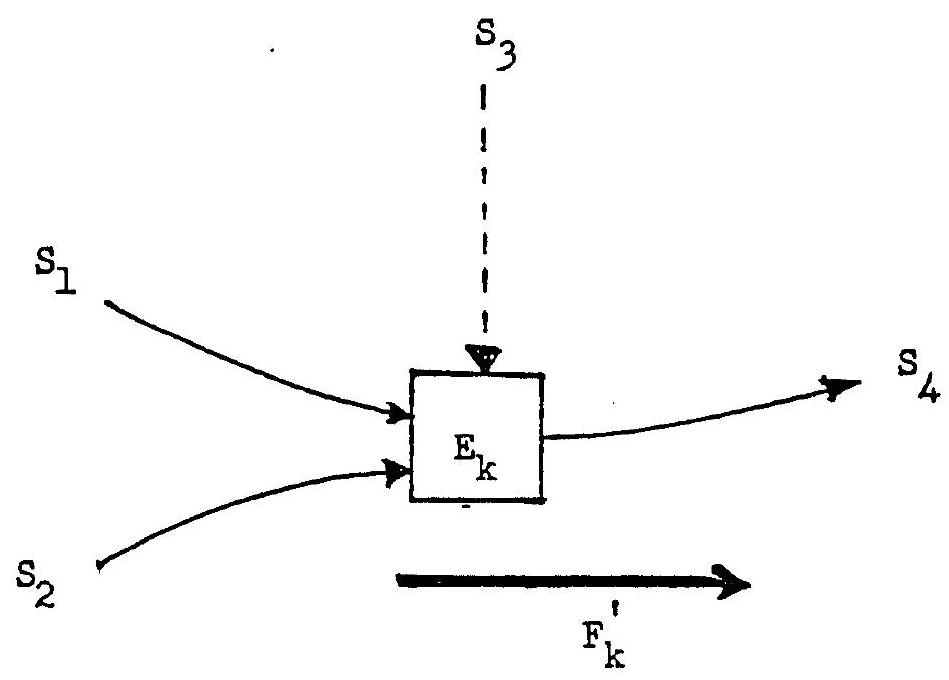
\includegraphics[max width=0.6\textwidth]{2023_01_30_a974a42f7b7381f3f940g-121}
\end{center}

Suppose that the $\alpha$ of the $j$th block is modulated by $\frac{\Delta \alpha_{j}}{\alpha_{j}}$, then considering the whole system.
%
\begin{equation}
\frac{\Delta F_{k}^{\prime}}{F_{k}^{\prime}}= C_{\alpha_{j}}^{F_{k}^{\prime}} \cdot \frac{\Delta \alpha_{j}}{\alpha_{j}}, \frac{\Delta S_{1}}{S_{1}}=C_{\alpha_{j}}^{S_{1}} \cdot \frac{\Delta \alpha_{j}}{\alpha_{j}}, \ldots \text { etc. }
\label{eqn:334}
\end{equation}
%
Considering now the kth block in isolation we can write 99.
%
$$
\begin{aligned}
& \frac{\Delta F_{k}^{\prime}}{F_{k}^{\prime}}= \varepsilon_{\alpha_{j}}^{F_{k}^{\prime}} \cdot \frac{\Delta \alpha_{j}}{\alpha_{j}} + \varepsilon_{S_{1}}^{F_{k}^{\prime}} \frac{\Delta S_{1}}{S_{1}} + \varepsilon_{S_{2}}^{F_{k}^{\prime}} \cdot \frac{\Delta S_{2}}{S_{2}}+\ldots \\
& \text { Replacing the fractional changes by means of relations (3.34) this becomes } \\
& C_{\alpha_{j}}^{F_{k}^{\prime}} \cdot \frac{\Delta \alpha_{j}}{\alpha_{j}}=\varepsilon_{\alpha_{j}}^{F_{k}^{\prime}} \frac{\Delta \alpha_{j}}{\alpha_{j}}+ \varepsilon_{S_{1}}^{F_{k}^{\prime}} \cdot C_{\alpha_{j}}^{S_{1}} \cdot \frac{\Delta \alpha_{j}}{\alpha_{j}}+\ldots \\
& \text { Now } \varepsilon_{\alpha_{j}}^{F_{k}^{\prime}}=\delta_{j}^{k}, \frac{\Delta \alpha_{j}}{\alpha_{j}} \text { will cancel out and if we suppose, for example, } \\
& \text { that } C_{\alpha_{j}}^{S_{4}} \text { is unknown and the other coefficients are known we get: } \\
\end{aligned}
$$
%
\begin{equation}
C_{\alpha_{j}}^{S}=\left(C_{\alpha_{j}}^{F_{k}^{\prime}}-\delta_{j}^{k}- C_{\alpha_{j}}^{S_{1}} \cdot \varepsilon_{1}^{k}- C_{\alpha_{j}}^{S_{2}}: \varepsilon_{2}^{k}- C_{\alpha_{j}}^{S_{3}} \cdot \varepsilon_{3}^{k}\right) / \varepsilon_{4}^{k}
\label{eqn:335}
\end{equation}
%
Relations of type (3.35) and those discussed earlier can be used to progressively discover the sensitivity of measures from the known sensitivity of other measures and in many simple networks it is possible to obtain a complete sensitivity matrix in this way using only the known or estimated values of flux elasticities at the existing S.S.

\section{Application of theorems relating system coefficients to elasticities}

Some examples will now be given to make clear how sensitivity matrices may be computed from elasticities.

{\bf\large EXAMPLE I: Straight Chain with Multiple Inhibitory Loops}

Consider the straight chain system indicated below where values of elasticities around the S.S. working conditions of the transformation blocks are written inside brackets at the appropriate points in the diagram. Thus:

\begin{center}
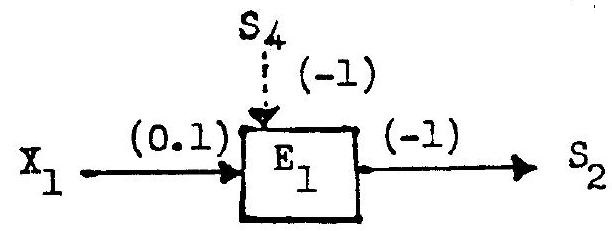
\includegraphics[max width=0.5\textwidth]{2023_01_30_a974a42f7b7381f3f940g-123}
\end{center}

means that the elasticities of enzyme 1 are: $0.1,-1,-1$, with respect to substances $\mathrm{X}_{1}, \mathrm{S}_{2}$ and $\mathrm{S}_{4}$ respectively. The negative values reflect the 'normal' behaviour that a product inhibits the forward reaction and that $S_{4}$ is a true inhibitor. The example includes three inhibitory loops, two of which are intersecting, to demonstrate how this affects the computation. Most of the elasticities have been taken as either $+1$ or -1, so that the arithmetic shall remain simple. Although quite feasible they are not intended to represent any real system.

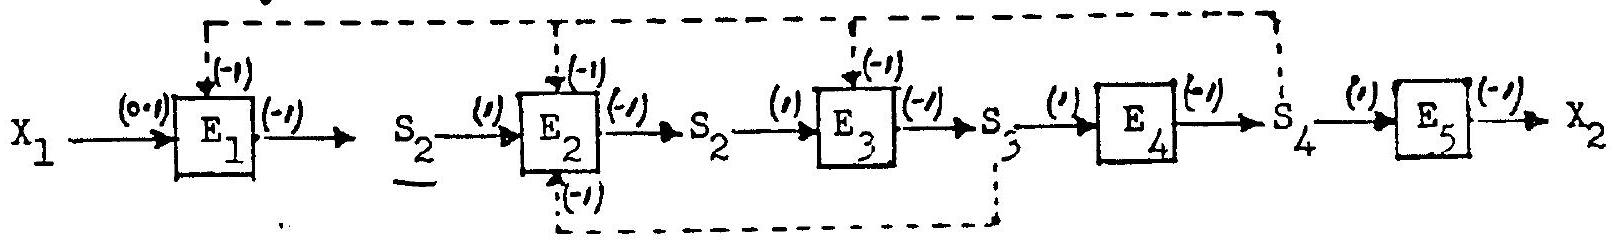
\includegraphics[max width=\textwidth, center]{2023_01_30_a974a42f7b7381f3f940g-123(1)}

The computation of a sensitivity matrix for the pools and for the pathway flux,$\left[\begin{array}{c} C^{F, S_{i}}_{\alpha_j}\end{array}\right]$ proceeds as follows:

Assume $C_{\alpha_{1}}^{F}$ to be scaled to unity, then using relations of type (3.26) arising from the virtual modulation of pools we get 101.

from pool $S_{1}: \quad C_{2}=-C_{1} \times \frac{\varepsilon_{1}^{1}}{\varepsilon_{1}^{2}}$, where $\varepsilon_{1}^{1}$ stands for $\varepsilon_{1}^{F_{1}^{\prime}}$ and so on

or

$C_{2} = -(1) \times \frac{(-1)}{(1)}=1$

from pool $S_{2}: \quad C_{3}=-C_{2} \times \frac{\varepsilon_{2}^{2}}{\varepsilon_{2}^{3}}=1$

$$S_{3}: \quad C_{4} = -\frac{\left(\varepsilon^{2}_3 \cdot C_{2} + \varepsilon^{3}_3 \cdot C_{3}\right)}{\varepsilon^{4}_3} = C_{2}+ C_{3}=2$$

$$S_{4}: \quad C_{5} = -\frac{\left(\varepsilon_{4}^{1} C_{1}+\varepsilon_{4}^{2} C_{2}+ \varepsilon_{4}^{3} C_{3}+\varepsilon_{4}^{4} \cdot C_{4}\right)}{\varepsilon_{4}^{5}}$$

$$C_{5}=C_{1}+C_{2}+C_{3} + C_{4} = 5$$

The actual coefficients must satisfy the summation theorem (3.21) and can be found by normalising the numbers just discovered, which are proportional to the flux coefficients.

This gives
%
$$
\left[C_{1}, C_{2}, C_{3}, C_{4}, C_{5}\right]=[0.1, 0.1, 0.1, 0.2, 0.5]
$$
%
Having discovered the vector of flux coefficients with respect to the different blocks $C_{\alpha_{j}}^{F}$, we may use it to successively generate the vectors for pool coefficients in the order
%
$$ C_{\alpha_{j}}^{S_4}, C_{\alpha_{j}}^{S_{3}}, C_{\alpha_{j}}^{S_{2}}, C_{\alpha_{j}}^{S_{1}} \text { using relations of type (3.35) }
$$
%
arising from the consideration of the enzymes $\mathrm{E}_{5}, \mathrm{E}_{4}, \mathrm{E}_{3}, \mathrm{E}_{2}$ in isolation.

Thus for $E_{5}$ we get: $C_{\alpha_{j}}^{S_4}=\left(C_{\alpha_{j}}^{F}-\delta_{j}^{5}\right) / \varepsilon_{4}^{5}$

$\text{which generates the vector } C_{\alpha_j}^{S_4}=[0.1, 0.1, 0.1, 0.2, -0.5]$
%

For enzyme $E_{4}$ : $
C_{\alpha_{j}}^{S_{3}}=\left(C_{\alpha_{j}}^{F}-\delta_{j}^{4}-C_{\alpha_{j}^{4}}^{S} \cdot \varepsilon_{4}^{4}\right) / \varepsilon_{3}^{4}
$

generating $ C_{\alpha_{j}}^{S_{3}}=[0.2, 0.2, 0.2, -0.6, 0] $

For enzyme $E_{3}: \quad C_{\alpha_{j}}^{S_{2}}=\left(C_{\alpha_{j}}^{F}-\delta_{j}^{3}-C_{\alpha_{j}}^{S_{3}} \cdot \varepsilon_{3}^{3}-C_{\alpha_{j}}^{S^{4}} \cdot \varepsilon_{4}^{3}\right) / \varepsilon_{2}^{3}$

generating $ C_{\alpha_{j}}^{S_{2}}=[0.4, 0.4, -0.6, -0.2, 0] $

Finally using the relationship for either $E_{1}$ or $E_{2}$, which will yield

identical results, we get $C_{\alpha_{j}}^{S_{1}}=[0.8, -0.2, -0.2, -0.4, 0.]$

The general sequence of computation can be summarised as:

\begin{center}
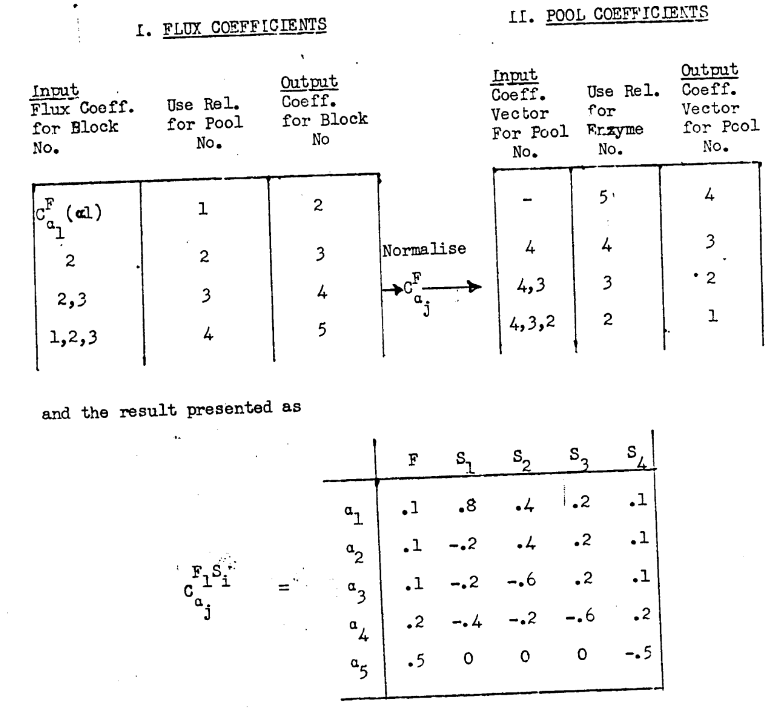
\includegraphics[max width=\textwidth]{figure3_ExampI.PNG}
\end{center}

Inspection of this matrix shows that various qualitative expectations are fulfilled. Thus a given pool always has positive coefficients for enzymes upstream from it and -ve coefficients for enzymes downstream. Furthermore all flux coefficients are +ve, as would be expected in a straight chain without positive feedback.

Two further examples follow, using the same format. These are intended to illustrate how quite complex networks can be dealt with and also to give some idea of the numerical range and the general pattern which sensitivity coefficient may take.

{\bf\large EXAMPLE II: Bimolecularly Coupled Pathways}

\begin{center}
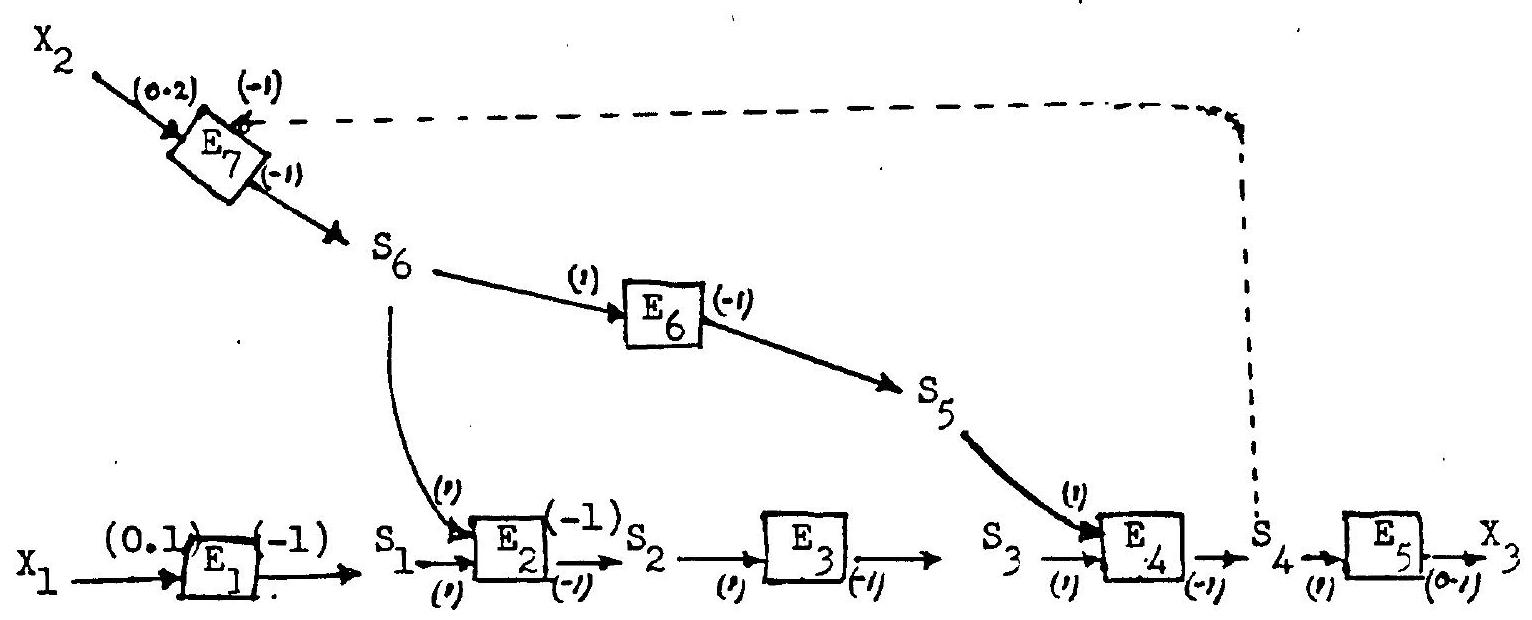
\includegraphics[max width=1\textwidth]{2023_01_30_a974a42f7b7381f3f940g-127(1)}
\end{center}

In this case the sequence of computation is:

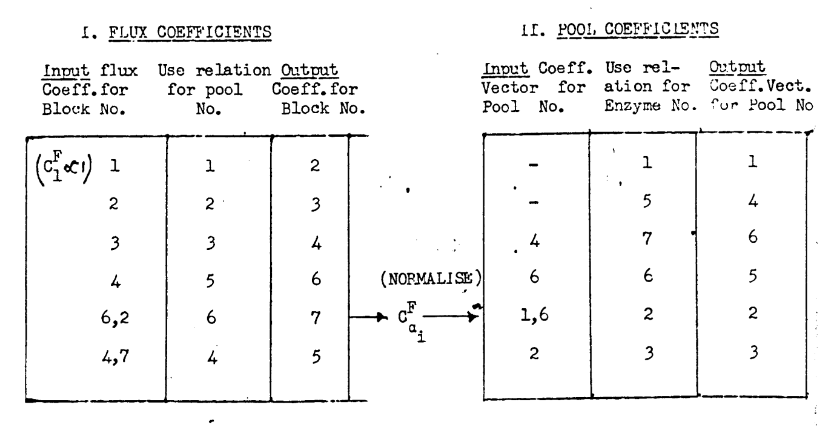
\includegraphics[max width=1.1\textwidth]{figure3_ExampII}

\begin{center}
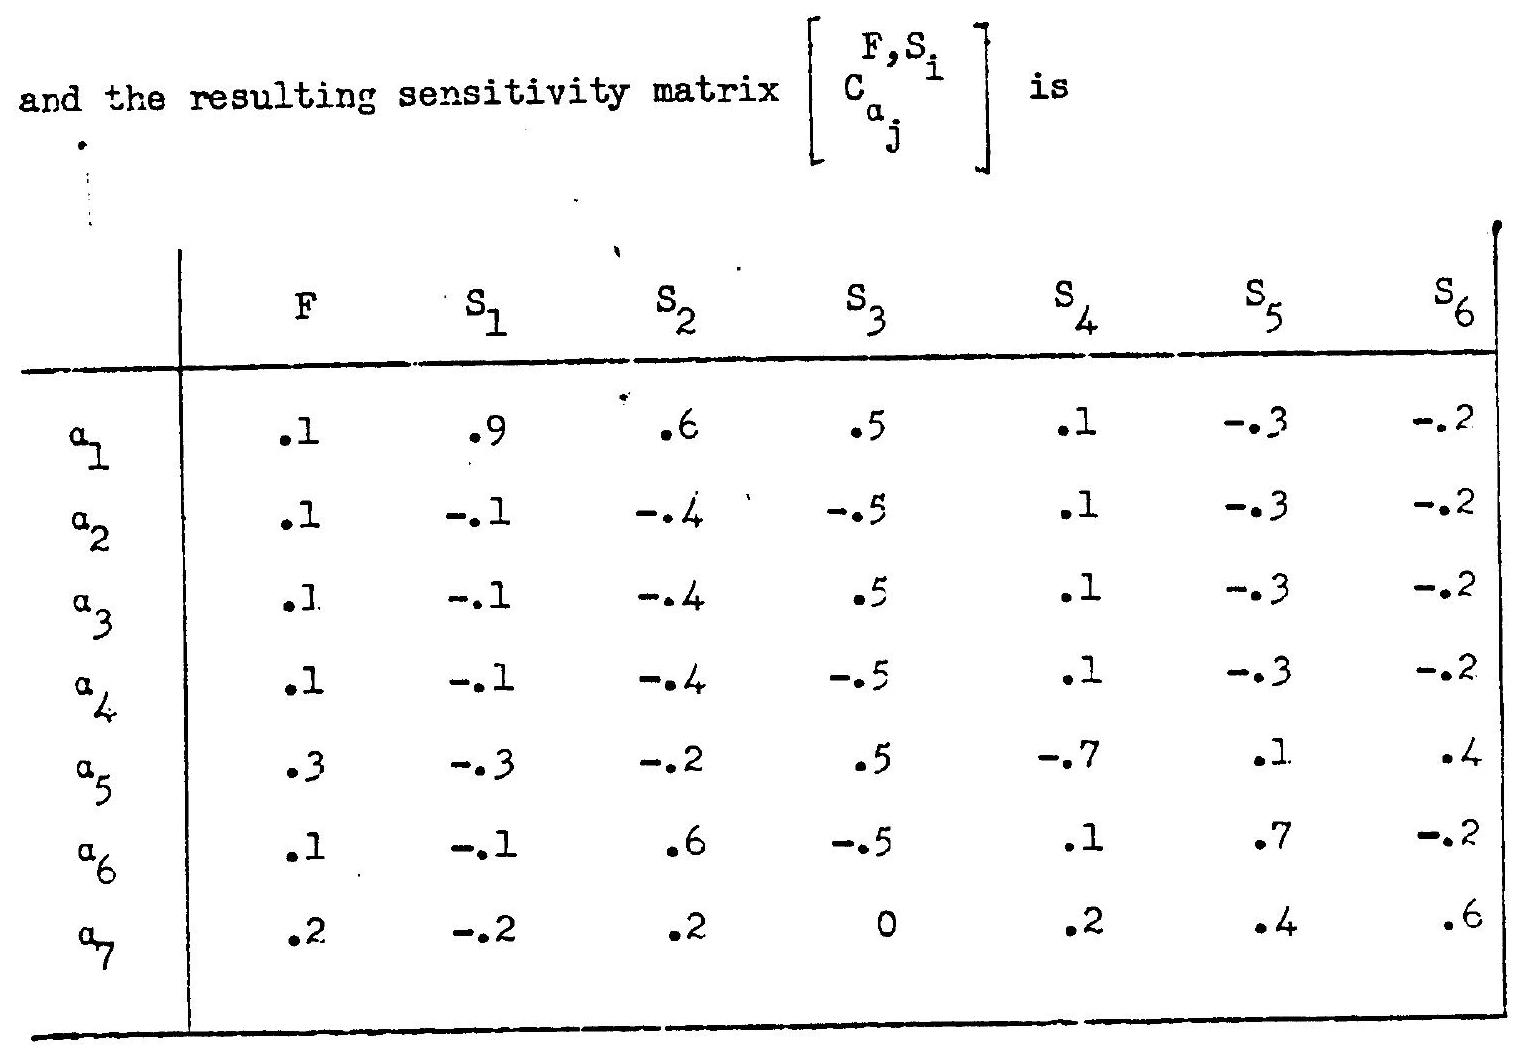
\includegraphics[max width=0.8\textwidth]{2023_01_30_a974a42f7b7381f3f940g-128}
\end{center}

{\bf\large EXAMPLE III: UREA TYPE CYCLE}

The two previous examples have considered 'uniflux' systems, that is systems characterised by $m-n=1$, and therefore possessing only one independent flux. For suck systems, once the $n$ relations of type (3.26) arising from pool modulations have been used, only one extra condition relating the coefficients was required and this condition was provided by the fact that $\sum C_{\alpha_{j}}^{F}=1$.

We now wish to consider systems with several independent fluxes where it will be necessary to use relations of type (3.33) which involve stoichiometric elasticities. As an example we will consider the system shown below which contains two independent fluxes $Y_{1}$ and $I_{2}$ and is similar to the urea cycle if $\mathrm{S}_{1}, \mathrm{S}_{2}, \mathrm{S}_{3}, \mathrm{S}_{4}$ stand respectively for ORN, CIT, ASA, ARG and $x_{2}$ is UREA. In order to define the stoichiometric elasticities it is necessary to know the ration $Y_{2} / Y_{1}$, i.e. the ratio of the flux round the cycle to the flux into protein and this is taken in this example to be $1 / 2$. As before all flux elasticities are taken to be $+1$ or $-1$ except for $\varepsilon_{1}^{6}$ which is taken as zero since this step is regarded as irreversible and $\varepsilon_{4}^{5}$ which is taken as $2 / 7$, again for arithmetic reasons.

\begin{center}
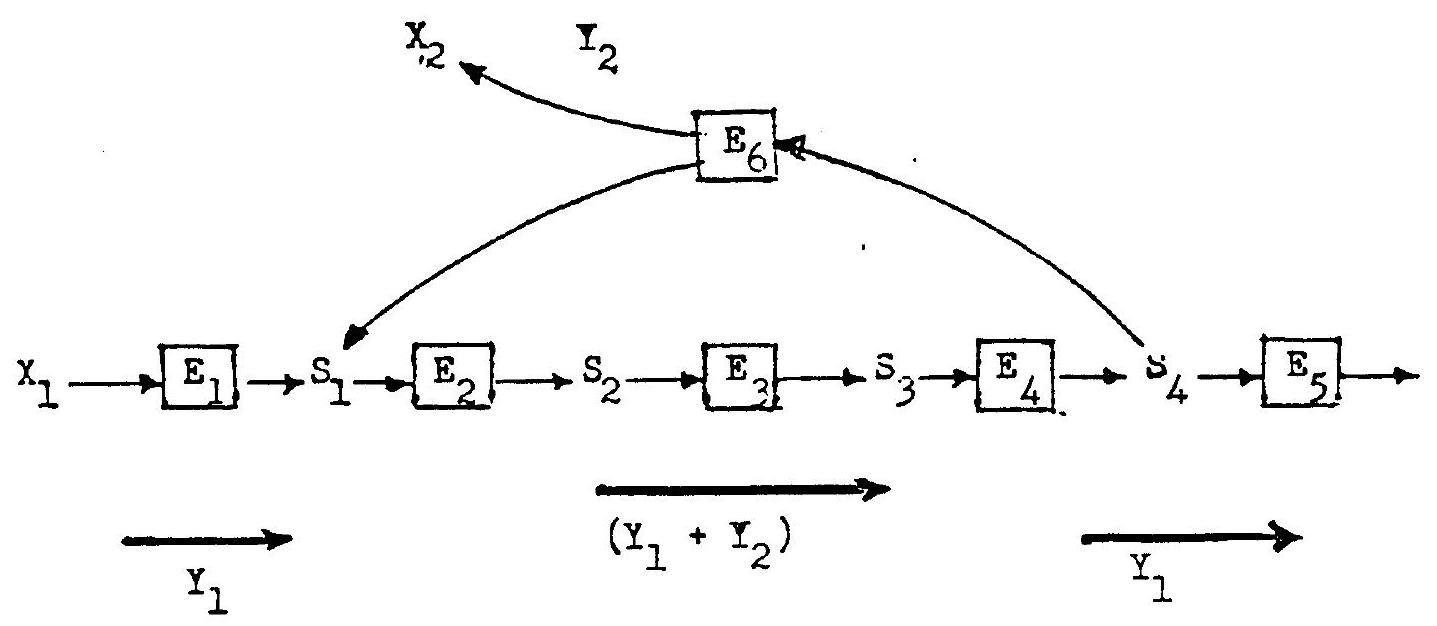
\includegraphics[max width=0.9\textwidth]{2023_01_30_a974a42f7b7381f3f940g-129}
\end{center}

Given then the ratio of the independent fluxes and the flux expression elasticities the computation of $\left[C^{Y_1,Y_2,S_i}_{\alpha_j}\right]$ proceeds as follows:

First of all we note that the stoichiometric elasticities of the local fluxes with respect to the independent fluxes can be written down by considering what fraction of a given flux is accounted for by a particular independent flux. This gives

$$ \varepsilon_{Y}^{F_j} \quad = [1, 2/3, 2/3, 2/3, 1, 0] $$

$$\mbox{ and } \varepsilon_{Y}^{F_2} \quad = [0, 1/3, 1/3, 1/3, 0, 1] $$

Considering first the sensitivity of the independent flux $Y_{1}$ to the separate blocks, let us suppose that $C^{Y_1}_1 = x$. Then the pool relationships for $S_{1} S_{2} S_{3}$ show that $C_{1}^{Y}=C_{2}^{Y_{1}}=C_{3}^{Y_{1}}=C_{4}^{Y_{1}}=x$ Suppose further that $C_{5}^{Y}=y$ and $C_{6}^{Y_{I}}
=2$

We can now use the relation for pool $\mathrm{S}_{4}$ to give
%
$$
(-1) \cdot x+(2 / 7) \cdot y+(1) \cdot z=0
$$
%
and the flux modulation relations of type (3.33), where modulation of $Y_{2}$ gives
%
$$
1 / 3 \cdot x+1 / 3 \cdot y+1 / 3 \cdot x+(1) \cdot z=0
$$
%
and modulation of $Y_{1}$ gives
%
$$
(1) \cdot x+2 / 3 \cdot x+2 / 3 \cdot x+2 / 3 \cdot x+(1) \cdot y=1
$$
%
These three equations are easily solved to yield
%
$$
x=0.1, y=0.7, z=-0.1
$$
%
or
%
$$
C_{\alpha j}^{Y_{1}}=[0.1, 0.1, 0.1, 0.1, 0.7, -0.1]
$$
%
A similar argument then yields $\mathrm{C}_{\alpha_j}^{\mathrm{Y_2}}=[0.35, 0.35, 0.35, 0.35, -1.05, 0.65]$ Before proceeding to discover the $C_{\alpha_j}^{S_{i}}$ using enzyme equations of type (3.35) it is necessary to know the sensitivity to each of the $\alpha_{j}$ of the flux carried by each enzyme. This has already been established for $E_{1}$, $E_{5}, E_{6}$, but we still require the sensitivities for $E_{2}, E_{3}, E_{4}$ which all carry the flux $\left(Y_{1}+Y_{2}\right)$.

This can be written down using the relation (3.10) proved earlier for a branched pathway.
%
$$C_{\alpha_{j}}^{\left(Y_{1}+Y_{2}\right)}=\frac{Y_{1}}{Y_{1}+Y_{2}} C_{\alpha_{j}}^{Y_{1}}+\frac{Y_{2}}{Y_{1}+Y_{2}} \cdot C_{\alpha_{j}}^{Y_{1}} = 2/3 C_{C_{\alpha_j}}^{Y_{1}}+1 / 3 C_{\alpha_{i}}^{Y_{2}}$$
%
or
%
$$\mathrm{C}_{\alpha_{j}}^{\left(Y_{1}+Y_{2}\right)} = [0.183, 0.183, 0.183, 0.183, 0.183, 0.116, 0.150]$$
%
From this point it is straightforward to obtain the $C_{\alpha_{j}}^{S_{1}}, C_{\alpha_{j}}^{S}, C_{\alpha_{j}}^{3} C_{\alpha_j}^{S}$ using successively the relation of type (3.35) for $\mathrm{E}_{1}, \mathrm{E}_{2}, \mathrm{E}_{3}, \mathrm{E}_{4} \cdot$ In this case it is important to remember that the term $C_{\alpha_{j}}^{F_{k}^{\prime}}$ in (3.35) refers in each case to tho flux carried by the particular enzyme which is involved.

\begin{center}
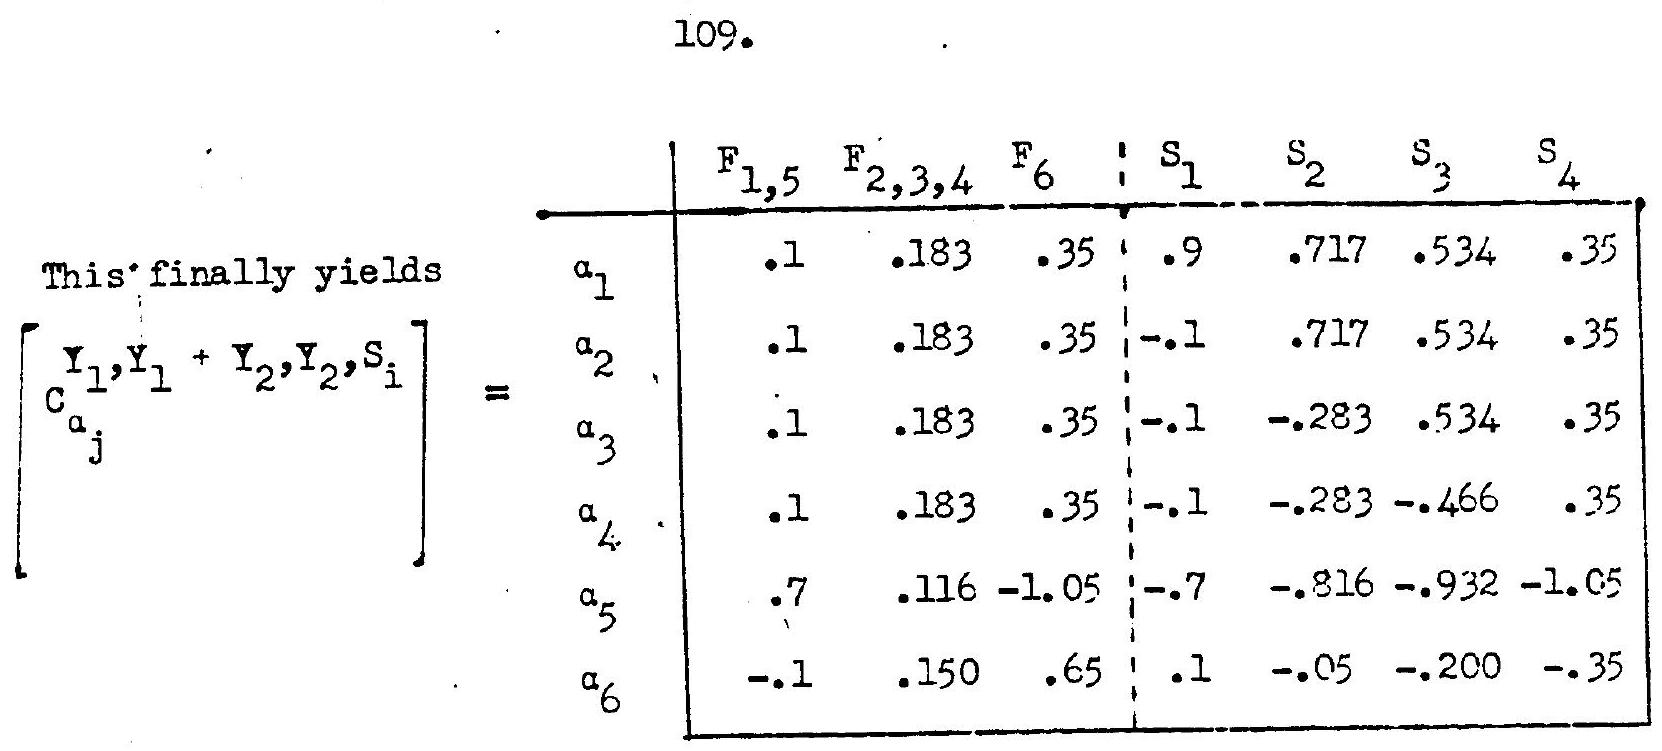
\includegraphics[max width=0.9\textwidth]{2023_01_30_a974a42f7b7381f3f940g-132}
\end{center}

Suppose now that it is required to know the sensitivity of the internal pools and fluxes to the level of $\mathrm{X}_{1}$. To obtain this we can use the relation (3.16) and, since the parameter $X_{1}$ only occurs in the block characterised by $\alpha_{1}$, we have
%
\begin{equation}
C_{X_{1}}^{M} = C_{\alpha_{1}}^{M_{1}} \cdot C_{X_{1}}^{F_{1}} = C_{\alpha_{1}}^{M} \cdot \varepsilon^{1}_{X_1}
\label{eqn:336}
\end{equation}
%
Noting from the diagram that the 1st block is rather saturated with respect to $X_{1}$, having an elasticity of only $0.1$, we can use the first row of the sensitivity matrix, together with $(3.36)$ to obtain
%
$$
\dot{C}_{X_{1}}^{F_{1,5}, F_{2, 3, 4}, F_{6}, S_{i}} = 0.01,\ 0.0183,\ 0.035,\ 0.09,\ 0.0717,\ 0.0534,\ 0.0351
$$
%
The above consideration shows that for a given S.S. system a knowledge of the relative values of the fluxes and of the elasticities of the separate flux expression at their working position is sufficient to determine the sensitivity matrix. In the examples given the task of calculating the sensitivity matrix from known. flux and stoichiometric elasticities was always straightforward. This was because the relatively simple `structure' of the systems under consideration gave rise in each case to a set of $m$ equations which could be solved by inspection.

\section{General limitations on coefficient values}

Previously we have seen that in certain uniflux systems we were able to state a general limit for the value of flux coefficients. These are systems in which all the $C_{\alpha_{j}}^{F}$ are necessarily + $v e$, when it follows that $0<C_{\alpha}^{F}<1$ for all j. No limitations were present for the pool coefficients. However, as soon as -ve coefficients become possible, either because of branching or perhaps, even in a uniflux system, when certain types of inhibition are operative, it is no longer clear that there are any such limits. Since it is not easy to consider this question in a general way we shall look instead at what limitation may exist in particular systems.

\section{Pool sensitivities in a chain of saturable enzymes}

Consider the simplest possible case; shown below, in which there is just one pool S. We wish to consider what limits are imposed on $C_{1}^{S}$.

\begin{center}
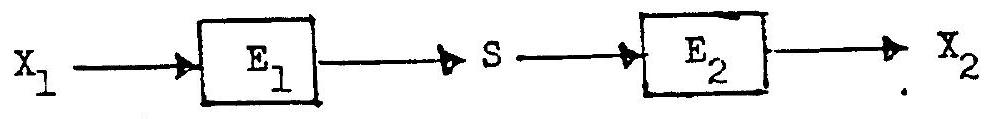
\includegraphics[max width=0.8\textwidth]{2023_01_30_a974a42f7b7381f3f940g-133(1)}
\end{center}

Clearly, by manipulating the relative quantity of $\mathrm{E}_{1}$ and $\mathrm{E}_{2}, \mathrm{S}$ car be anywhere within the range $X_{1} > S>  X_{2}$ (where the a are scaled concentrations taking account of the equilibrium constants). From the point of view of discussing the extreme, values of $C_{\alpha_{1}}^{S}$ and $C_{\alpha_{2}}^{S}$ we may take $S$ as being variable within this range.

Now using our previous theorem $(3.26)$ and denoting the elasticities by $\varepsilon_{S}^{1}$ and $\varepsilon_{S}^{2}$ we can write
%
$$
\mathrm{C}_{\alpha_{1}}^{F} \cdot \varepsilon_{S}^{1}+\mathrm{C}_{\alpha_{2}}^{F} \cdot \varepsilon_{S}^{2} = 0
$$
%
also $C_{\alpha_{1}}^{F} + C_{\alpha_{2}}^{F}=1$

so that $C_{\alpha_{1}}^{F}=\frac{\varepsilon_{S}^{2}}{\varepsilon_{S}^{2}-\varepsilon_{S}^{1}}$

and $\quad C_{\alpha_{1}}^{S} = C_{\alpha_{1}}^{F} / \varepsilon_{S}^{2}=\frac{1}{\varepsilon_{S}^{2}-\varepsilon_{S}^{1}}=-C_{\alpha_{2}}^{S}$

Clearly we car go no further without considering the form of the saturable rate expressions $f_{1}, f_{2}$ for the two enzymes. Let us assume that these are the simplest which will take saturation and reversibility fully into account, viz:
%
$$
\begin{aligned}
& f_{1}=\frac{X_{1}-S}{1+\frac{1}{M_{1}}+\frac{S}{M_{1}^{\prime}}} \\[6pt]
& f_{2}=\frac{S-X_{2}}{1+\frac{S}{M_{2}}+\frac{X_{2}}{M_{2}^{\prime}}}
\end{aligned}
$$
%
Where $M_{1}^{\prime}$ and $M_{2}^{\prime}$ are the `reverse' Michaelis constants. then using the formal relation, $C_{P}^{M_{1} / M_{2}}=C_{P}^{M_{1}}-C_{P}^{M_{2}}$, and finding the coefficients of the numerator and denominator by differentiation we have
%
\begin{align*}
\varepsilon_{S}^{1} &= C_{S}^{f_1} = -\left[\frac{S}{X_{1}-S}+\frac{S / M_{1}^{\prime}}{1 + X/M_{1} + S/M_{1}^{\prime}}\right] = -(a+b) \\
%
\mbox{ and } \varepsilon_{S}^{2} &= C_{S}^{f_{2}} = \left[\frac{S}{S - X_{2}}-\frac{S/M_{2}}{1+ S/M_{2} + X_{2}/X_{2}^{\prime}}\right] = (c-d)
\end{align*}

Where $a, b, c$, d represent the appropriate algebraic groupings. Clearly $a$ and $c$ represent components of the elasticity which depend mainly on `out of equilibriumness' of the reaction whereas $b$ and $d$ are concerned with the degree of saturation of the reaction. Inspection shows that
%
$$
0<a<\infty, \quad 1<c<\infty, \quad 0<b<1, \quad 0<d<1
$$
%
and that when the reaction steps are close to equilibrium the saturation term will be unimportant. Using this notation we have
%
$$
\begin{aligned}
C_{\alpha_{1}}^{S} &=\frac{1}{\varepsilon^{2}-\varepsilon^{1}} \\[4pt]
C_{\alpha_{1}}^{S} &=\frac{1}{a+b+c-d} \hspace{12PT}\mbox{and it is easy to establish} \\[4pt]
C_{\alpha_{1}}^{S} &>0
\end{aligned}
$$
%
Is there any upper bound for $\mathrm{C}_{\alpha_{1}}^{\mathrm{S}}$ ? The problem is to consider the maximum value of $C_{\alpha_{1}}^{S}$ for any values of $M_{1}, M_{1}^{\prime}, M_{2}, M_{2}^{\prime}$ and any value of $S$ in the range $X_{1}> S > X_{2}$

We require a `minimum' of $(a+b+c-d)$ and this will be so when

\begin{enumerate}[label=(\roman*),parsep=-3pt]
\item d is maximal, $=1$, i.e. $E_{2}$ fully saturated

\item b is minimal, $=0$, i.e. $E_{1}$ fully unsaturated
\end{enumerate}

This merely requires sufficiently extreme values of $M_{1}^{\prime}$ and $M_{2}$ and can be satisfied regardless of the value of S.

(iii) S lies at a value which will minimise $(a+c)$

$\displaystyle \mbox{Now} \quad a+c=\frac{S}{X_{1}-S}+\frac{S}{S-X_{2}} $

and it can be shown that the minimum occurs at $S = \sqrt{X_{1} \cdot X_{2}}$ So that
%
$$
\begin{aligned}
\left(C_{\alpha_{1}}^{\mathrm{S}}\right)_{\max } & =\frac{1}{(a+c)_{\min}+0-1} \\[6pt]
& =1 / 2\left(\sqrt{\frac{\mathrm{X}_{1}}{\mathrm{X}_{2}}}-1\right)
\end{aligned}
$$
%
At this maximum position the value of the flux coefficient is
%
$$
\mathrm{C}_{\alpha_{1}}^{\mathrm{F}} = 0.5
$$
%
Thus we have established that in the absence of any knowledge other the than a general form for the saturable expression and the values of $X_{1}, X_{2}$
%
$$
0 < C_{\alpha_{1}}^{S} < 1/2\left(\sqrt{\frac{X_{1}}{X_{2}}}-1\right)
$$
%
Clearly then if $X_{1} \gg X_{2}$ there is no effective limit to the value of $C_{\alpha_{1}}^{S}$ and we may expect that under certain circumstances very large values of pool coefficients could occur.

In particular a large pool coefficient appears likely whenever a saturated and almost irreversible enzyme appears at the end of a chain and when the flux control is shared equally between it and the rest of the chain.

\section{Pool sensitivities in a chain of linear enzymes}

In the case of two linear enzymes an almost identical argument applies, except that the saturation components of the elasticities are absent so that
%
$$
C_{\alpha}^{S}=\frac{1}{a+c}
$$
%
Once again the minimum occurs when $S=\sqrt{X_{1} X_{2}}$

\medskip
and gives the result $0 < C_{\alpha}^{S}<\frac{\sqrt{X_{1}}-\sqrt{X_{2}}}{\sqrt{X_{1}}+\sqrt{X_{2}}}$, so that $C_{\alpha}^{S} < 1$

\medskip
the value of $C_{\alpha_{1}}^{F}$ at this maximum is $C_{\alpha_{1}}^{F} \bumpeq \frac{\sqrt{X_{1}}}{\sqrt{X_{1}}+\sqrt{X_{2}}}$

\medskip
$ \displaystyle \text { For example if } \mathrm{X}_{1}=100, \mathrm{X}_{2}=1,\left(C_{\alpha}^{S}\right)_{\max }=\frac{10 -1}{10+1}=82 \% $

\medskip
$ \displaystyle \text { at which position } C_{\alpha_{1}}^{F} \bumpeq \frac{10}{10+1}=90 \% \text { This indicates that the } $

\medskip
$ \displaystyle \text { result } C_{\alpha_{1}}^{F}=0.5 $  for the saturable case is not general and, more importantly, we have demonstrated that in a chain of linear enzymes the  pool coefficients are strictly bounded.


\section{Flux coefficients}

The results just proved for pool coefficients can be used to show that in systems with branching, that is with more than one independent flux, there is no a priori limit on the values of flux coefficients as there is for a straight chain of enzymes.

Consider the branching system shown below, where $E_{1}$ and $E_{2}$ may be saturable enzymes.

\begin{center}
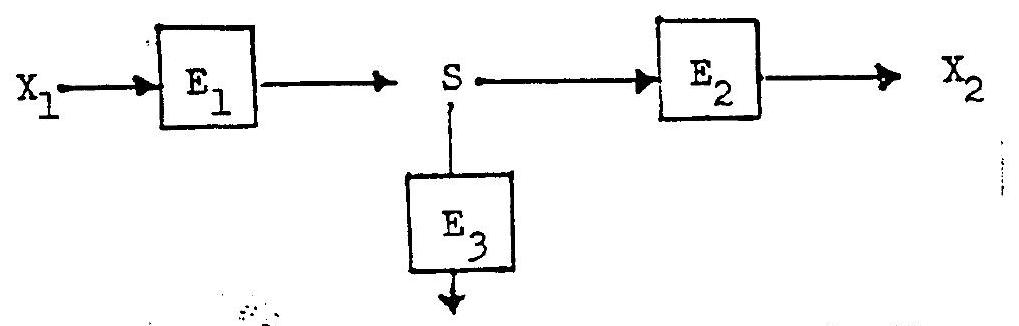
\includegraphics[max width=0.7\textwidth]{2023_01_30_a974a42f7b7381f3f940g-138}
\end{center}

Let us suppose that the enzyme $E_{3}$ is effectively linear and irreversible and that the flux through it, $F_{3}$, is small compared with the fluxes $F_{1}$ and $F_{2}$ in the main pathway.

Under these circumstances it follows that $\mathrm{C}_{\alpha_{1}}^{\mathrm{F}_{3}} \bumpeq \mathrm{C}_{\alpha_{1}}^{\mathrm{S}}$ and, from the result just proved for a chain of two saturable enzymes, also
%
$$
\left(C_{\alpha_{1}}^{S}\right)_{\max } \bumpeq 1/2\left(\sqrt{\frac{X_{1}}{X_{2}}}-1\right)
$$
%
Thus
%
$$
\left(C_{\alpha_{1}}^{F_3}\right)_{\max} \bumpeq 1/2\left(\sqrt{\frac{X_{1}}{X_{2}}}-1\right)
$$
%
This demonstrates that very large + or -ve values of flux coefficients are possible in a branching system which contains saturable enzymes.

It will be noticed, however, that this result is for the coefficient of a flux with respect to an enzyme not directly in the pathway carrying the flux. In fact it is often possible to identify, within a larger system, major pathways which carry a flux large by comparison with any branches from them. The coefficients of the flux ir: such major pathways with respect to the enzymes actually in them will under normal circumstances still satisfy the limitation $0 < C_{\alpha}^{F} < 1$

\section{`Diagnostics' for rate control in non-linear systems}

In $\mathrm{Ch}$ I it was shown, for a sequence of linear enzymes, that the difference in pool levels across enzymes in a chain was Iror.rrtional to their respective flux coefficients, $C_{\alpha_{i}}^{F}$, provided the pool concentrations were scaled to take account of the product of equilibrium constants along the chain. Thus the pattern of scaled pool levels at the S.S. could be used as a simple diagnostic for rate control. We now wish to consider how this simple diagnostic for rate control in a chain of enzymes will be altered when allowance is made for enzymes having saturable rate expressions.

\begin{center}
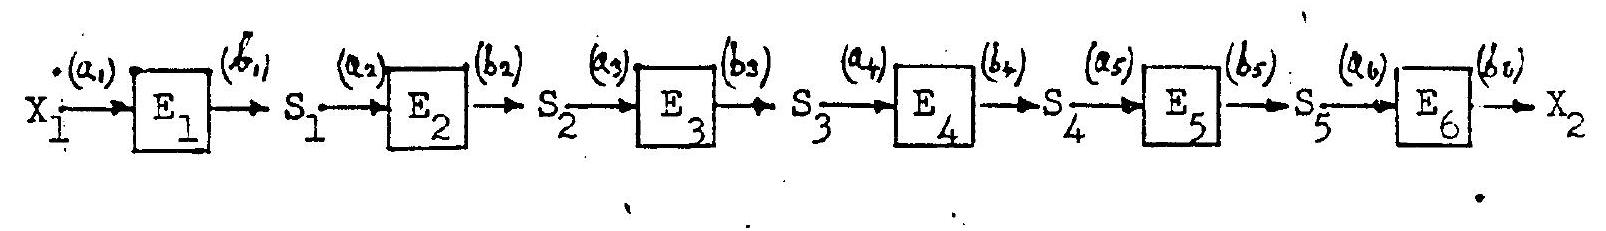
\includegraphics[max width=\textwidth]{2023_01_30_a974a42f7b7381f3f940g-140}
\end{center}

Such a system is shown above and the substrate and product elasticities `a' and `b' respectively, are written next to each enzyme using the appropriate suffixes. By using the pool modulation relations (3.26) and arbitrarily taking the unnormalised value of the 1st flux coefficient, $C_{1}$, as $1/a_{1}$ we can show that:
%
\begin{equation}
\left[C_{1}, C_{2}, C_{3}, \ldots\right] \propto\left[\frac{1}{a_{1}}, \quad \frac{1}{a_{2}}\left(-\frac{b_{1}}{a_{1}}\right), \quad \frac{1}{a_{3}}\left(-\frac{b_{1}}{a_{1}}\right)\left(-\frac{b_{2}}{a_{2}}\right), \ldots \ldots \ldots\right]
\label{eqn:339}
\end{equation}
%
This shows that the elasticities of a given enzyme, say $E_{3}$, affect its own coefficient directly through the factor $\frac{1}{a_{3}}$ and indirectly by multiplying all terms 'downstream' from it by the factor $\left(-\frac{b_{3}}{a_{3}}\right)$. In order to proceed further we must now assume the simplest rate expression which will adequately represent the saturability and reversibility of the typical step shown below.

\begin{center}
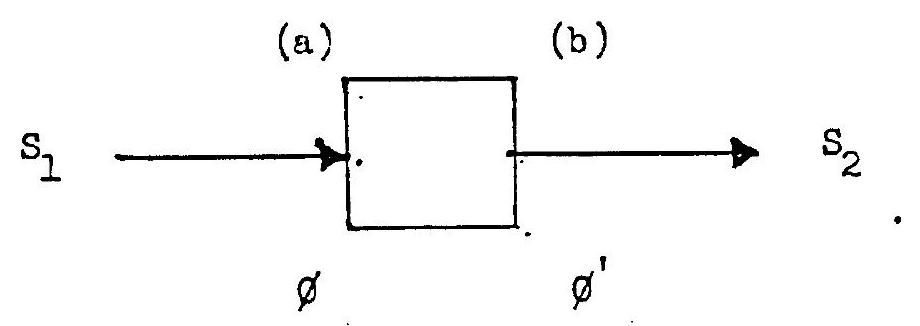
\includegraphics[max width=0.9\textwidth]{2023_01_30_a974a42f7b7381f3f940g-140(1)}
\end{center}

If $S_{1}$ and $S_{2}$ are suitably scaled so that the equilibrium constant is eliminated such an expression will be
%
\begin{equation}
F=\frac{\frac{\mathrm{V}}{\mathrm{M}}\left(\mathrm{S}_{1}-S_{2}\right)}{I+\frac{S_{1}}{M}+\frac{S_{2}}{M^{\prime}}}=\frac{\frac{\mathrm{V}^{\prime}}{M^{\prime}}\left(S_{1}-
S_{2}\right)}{1+\frac{S_{1}}{M}+\frac{S_2}{M^{\prime}}}
\label{eqn:339}
\end{equation}
%
In this expression $V$ and $V^{\prime}$ represent the forward and reverse maximum velocities of the enzyme while $M$ and $M^{\prime}$ represent Michaelis constants for the substrate $S_{1}$ and the product $S_{2}$ respectively.

Using this rate equation it is now possible to write down the elasticities `a' and `b' with respect to $S_{1}$ and $S_{2}$ as
%
\begin{equation}
\begin{aligned}
& a =\frac{S_{1}}{S_{1}-S_{2}}-\frac{\frac{S_{1}}{M}}{1+\frac{S_{1}}{M}+\frac{S_{2}}{M^{\prime}}}=\frac{S_{1}}{S_{1}-S_{2}}- \phi \\
& b =-\frac{S_{2}}{S_{1}-S_{2}}-\frac{\frac{S_{2}}{M^{\prime}}}{1+\frac{S_{1}}{M}+\frac{S_{2}}{M^{\prime}}}=-\frac{S_{2}}{S_{1}-S_{2}}-\phi^{\prime}
\end{aligned}
\label{eqn:339}
\end{equation}
%
Where the terms $\phi$ and $\phi^{\prime}$, arising from the saturation property of the rate expression with regard to $S_{1}$ and $S_{2}$ respectively, are both positive and can be seen to satisfy the inequality $\left(\phi+\phi^{\prime}\right) < 1$. The latter condition means that it is impossible for  $\phi$ and $\phi^{\prime}$  to approach
their maximum values of unity simultaneously. The elasticities of (3.39) can be written as their 'linear' parts multiplied by correction
factors which differ from unity when saturation effects are important, thus
%
\begin{equation}
\begin{aligned}
& a = \frac{S_{1}}{S_{1}-S_{2}}\left(1-\phi \frac{S_1-S_2}{S_1}\right) \\
& b = -\frac{S_{2}}{S_{1}-S_{2}}\left(1+\phi^{\prime} \frac{S_{1}-S_{2}}{S_{2}}\right)
\end{aligned}
\label{eqn:340}
\end{equation}
%
Inspection of these correction factors indicates that the effect of saturation depends not only on the terms $\phi$ and $\phi^{\prime}$ but also on the equilibrium situation around the enzyme. For example if the `out of equilibrium ration, $\frac{S_{2}}{S_{1}}$, is close to unity the correction will be negligible even though one or other of the saturation terms may be at its maximal value.

The factors $\left(\frac{1}{a}\right)$ and $\left(-\frac{b}{a}\right)$ which occur for each enzyme in (3.37) can also be written as a `linear' part multiplied by correction factors $\beta$ and $\gamma$ respectively. Thus,
%
\begin{equation}
\frac{1}{a}=\frac{S_{1}-S_{2}}{S_{1}} \cdot \frac{1}{\left(1-\phi \frac{S_{1}-S_{2}}{S_{1}}\right)}=\frac{S_{1}-S_{2}}{S_{1}} \cdot \beta
\label{eqn:341}
\end{equation}
%
$$\left(-\frac{b}{a}\right)=\frac{S_{2}}{S_{1}} \cdot \frac{\left(1+\phi^{\prime} \frac{S_{1}-S_{2}}{S_{2}}\right)}{\left(1-\phi \frac{S_{1}-S_{2}}{S_{1}}\right)}=\frac{S_{2}}{S_{1}} \cdot \gamma
$$
%
Using the relation (3.41) with appropriate suffixes we can write (3.37) as
%
\begin{equation}
\left[C_{1}, C_{2}, C_{3}, \cdots\right] \cdot \left[\frac{X_1-S_1}{X_1} \cdot \beta_1, \frac{S_1-S_2}{X_1} \cdot \beta_2 \cdot \gamma_1, \frac{S_2-S_3}{X_1} \cdot \beta_3 \cdot \gamma_1 \cdot \gamma_2, \cdots \cdot\right]
\label{eqn:342}
\end{equation}
%
In the linear case, when $\phi=\phi^{\prime}=0$ for all enzymes, all $\beta$ and $\gamma$ terms in (3.42) are unity and the successive flux coefficients are just proportional to the scaled pool differences, confirming the result of CH.I. When however saturation effects are important it will be necessary to have some estimate of the factors $\beta$ and $\gamma$ in addition to the ratios of scaled pool levels which were a sufficient diagnostic in the linear case.

One possible way of estimating. the correction factor $\beta$ for an enzyme would be to use the definition, from (3.41), of
%
\begin{equation}
\beta=\frac{1}{1-\phi \frac{S_{1}-S_2}{S_1}}=\frac{1}{1-\frac{\frac{S_1}{M}}{1+\frac{S_1}{M}+\frac{S_2}{M^{\prime}}} \times\left(\frac{S_1-S_2}{S_1}\right)}
\label{eqn:341}
\end{equation}
%
However this would involve making a close study of each enzyme, to determine the Michaelis constants $M$ and $M^{\prime}$, and also a knowledge of \underline{absolute} pool levels rather than ratios.

Alternatively we may note from (3.38) that
%
$$\frac{F}{V}=\left(\frac{S_1}{M} \big/\left(1+\frac{S_1}{M}+\frac{S_2}{M^{\prime}}\right)\right) \quad \times \quad \frac{S_1-S_2}{S_1} = \phi \cdot \frac{S_1-S_2}{S_1}$$
%
so that
%
\begin{equation}
\beta=\frac{1}{1-\phi \frac{S_{1}-S_{2}}{S_{1}}}=\frac{1}{1-\frac{F}{V}}
\label{eqn:344}
\end{equation}
%
and similarly we can show that
%
\begin{equation}
 \gamma = \frac{1 + \frac{F}{V^\prime}}{1-\frac{F}{V}}
\label{eqn:345}
\end{equation}
%
Thus estimates for $\beta$ and $\gamma$ can be made by measuring the flux $F$ for unit weight of the organism and dividing it by the maximum activity in the forward and reverse directions of the enzyme extracted from unit weight, forming the required factors $\frac{F}{V}$ and $\frac{F}{V^\prime}$.

In principle, then, $\dot{a}$ knowledge for each enzyme of pool ratios and of in vivo flux against maximum flux can be used to diagnose relative flux control using the following relation, obtained by substituting the expressions (3.44) and (3.45) for $\beta$ and $\gamma$ into (3.42). Thus we have
%
\begin{equation}
\begin{split}
  \left[C_{1}, C_{2}, C_{3}, \cdots\right] &\propto  \left[ \frac{X_{1}-S_{1}}{X_{1}} \frac{1}{\left(1-\frac{F}{V_{1}}\right)},
%
\frac{S_1-S_2}{X_1}  \frac{1}{\left(1-\frac{F}{V_2}\right)}  \frac{\left(1+\frac{F}{V_1}\right)}{\left(1-\frac{F}{V_1}\right)}, \right. \\[7pt]
%
&\left. \frac{S_2-S_3}{X_0} \frac{1}{\left(1-\frac{F}{V_3}\right)}\left(\frac{1+\frac{F}{V_{1}^{\prime}}}{1-\frac{F}{V_1}}\right), \ldots \hspace{14pt}  \right]
\end{split}
\label{eqn:346}
\end{equation}
%
The pattern of pools around an enzyme in fact imposes limits on the values which $\beta$ and $\gamma$ can assume. Thus inspection of the expression (3.44) reveals that, for a given value of $S_{1}$ and $S_{2}, \beta$ will be a maximum when the forward saturation, $\phi$, approaches unity and a minimum when $\phi$ approaches zero. So that
%
\begin{equation}
1 < \beta < \frac{S_{1}}{S_{2}}
\label{eqn:347}
\end{equation}
%
A similar but rather more complex argument for (3.45) shows that $\gamma$ approaches a maximum when $\left(\phi+\phi^{\prime}\right)$ approaches unity, irrespective of the separate values of $\phi$ and $\phi^{\prime}$. So that we also have
%
\begin{equation}
1 < \gamma < \frac{S_{1}}{S_{2}}
\label{eqn:348}
\end{equation}
%
When attempting to estimate flux coefficients from a given set of pool data a useful first step is to take them as proportional to scaled pool differences, using the linear enzyme assumption. If additional evidence indicates that an enzyme may be saturated the effect of allowing for this will be to increase the value of the coefficient of all enzymes downstream from it by the common factor, $\gamma$, and also to increase its own coefficient by the factor $p$, which will be greater than unity and may approach $\frac{S_1}{S_2}$ if the saturation is predominantly forward. The inequalities established for $\beta$ and $\gamma$ indicate that it will only be important to allow for saturation effects at steps having a large 'out of equilibrium' ratio, $\frac{S_1}{S_2}$.

For example if all enzymes were known to be saturated from in front, in the sense that they had $\phi=1$, the application of (3.42) would give
%
$$
\left[C_1, C_2, C_3, C_4, C_5, C_6\right] \propto\left[\frac{X_1-S_1}{S_1}, \frac{S_1-S_2}{S_2}, \frac{S_2-S_3}{S_3}, \frac{S_3-S_4}{S_4}, \frac{S_4-S_5}{S_5}, \frac{S_5-X_2}{X_2}\right]
$$
%
Clearly if $\frac{X_1}{X_2}$ is close to unity, that is the whole chain is close to equilibrium, then a prediction based on the linear assumption will be good. If, however, $\frac{X_1}{X_2}$, is large then enzymes further down the chain may have much greater coefficients than would be expected on a linear hypothesis.

In particular whenever $X_1$ is close to zero, rendering the last step irreversible, the degree of saturation of the last step becomes of critical importance.

\section{Pools attenuate with metabolic distance}

{\bf Does the effect on pools attenuate with metabolic distance from the site of a modulation?}

We are now in a position to consider this question, for our straight chain of non-linear enzymes, taking the modulation to act on the quantity of some enzyme within the chain and 'metabolic distance' to be the number of enzymes between the modulation and the pool in question. Show below is a typical enzyme in the chain, not subject to modulation, and across which such 'attenuation' might occur once again, `a' and `b' indicate the appropriate elasticities.

\begin{center}
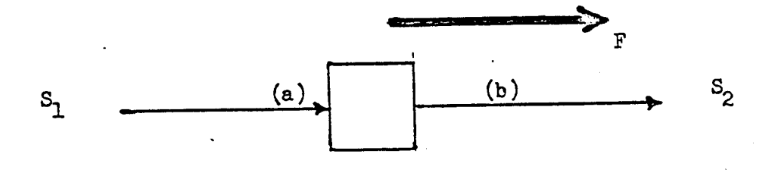
\includegraphics[scale=0.8]{figure3_Chain1.png}
\end{center}

Denoting the coefficients of the pools and of the flux, F, with respect to the remote modulated enzyme as $C_{1}, C_{2}$ and $C_{F}$ respectively it is convenient to consider $C_{1}$ and $C_{2}$ in terms of their deviations $\Delta_{1}$ and $\Delta_{2}$ from $C_{F}$, the flux coefficient $C_{F}$ being, of course, the same no matter which enzyme in the chain is considered. Thus
%
$$
C_{1} = C_{F}+\Delta_{1} \quad \text { and } \quad C_{2}=C_{F} + \Delta_{2}
$$
%
We can then discover whether $\Delta$ increases or decreases on passing through a particular enzyme by applying an enzyme relationship of type (3.35), which gives
%
$$
C_1 = \left(C_F - b \cdot C_2\right) / a
$$
or
%
$$ C_F+\Delta_1 = \left(C_F-b\left(C_F+\Delta_2\right)\right) / a $$
%
so that
%
\begin{equation}
\Delta_1 = A \Delta_2 + B C_F
\label{eqn:349}
\end{equation}
%
where
%
$$
A = \left(-\frac{b}{a}\right) \text { and } B=\frac{(1-b-a)}{a}
$$
%
Clearly the increase or decrease of $\Delta$ on passing through an enzyme will depend on the values assumed by the factors $A$ and $B$. Assuming the non linear enzyme to be of the same form as in the last section we can use the results obtained there to discover the limits on the numbers $A$ and $B$ in terms of the pools $S_{1}$ and $S_{2}$ surrounding the given enzyme.
%
$$
\text { Thus we had, from }(3.41) \text {, that } A=\left(-\frac{\mathrm{b}}{\mathrm{a}}\right)=\frac{\mathrm{S}_{2}}{\mathrm{S}_{1}} \cdot \gamma
$$
%
and using the inequality (3.48), for $\gamma$, this yields
%
\begin{equation}
\frac{S_{2}}{S_{1}} < A < 1
\label{eqn:350}
\end{equation}
%
Also we have from (3.39) that
%
$$
(1-a-b)=1-\frac{S_{1}}{S_{1}-S_{2}}+\frac{S_{2}}{S_{1}-S_{2}}+\left(\phi+\phi^{\prime}\right) $$
%
which simplifies to
%
$$
(1-a-b) = \phi + \phi^{\prime}
$$
%
$ \displaystyle \text { using }(3.41) \text { to provide the factor }\left(\frac{1}{a}\right) \text { this gives } $
%
$$
B = \frac{1-a-b}{a}=\left(\phi+\phi^{\prime}\right) \cdot \frac{\left(S_{1}-S_{2}\right)}{S_{1}} \cdot \beta
$$
%
and finally using the inequality (3.47) for $\beta$ together with the fact that maximum $\beta$ coincides with maximum $\phi$ we have
%
\begin{equation}
0 < B < \frac{S_{1}-S_{2}}{S_{2}}
\label{eqn:351}
\end{equation}

In both of these inequalities the minimum value occurs when the enzyme is `linear', the maximum when it is fully saturated.

Referring to the chain of enzymes indicated in the diagram below, where the disturbance acts at $E_{4}$, it is now possible to see under what circumstances attenuation of the disturbance might be expected, by using the relation (3.49) together with the inequalities just established for $A$ and $B$.

\begin{center}
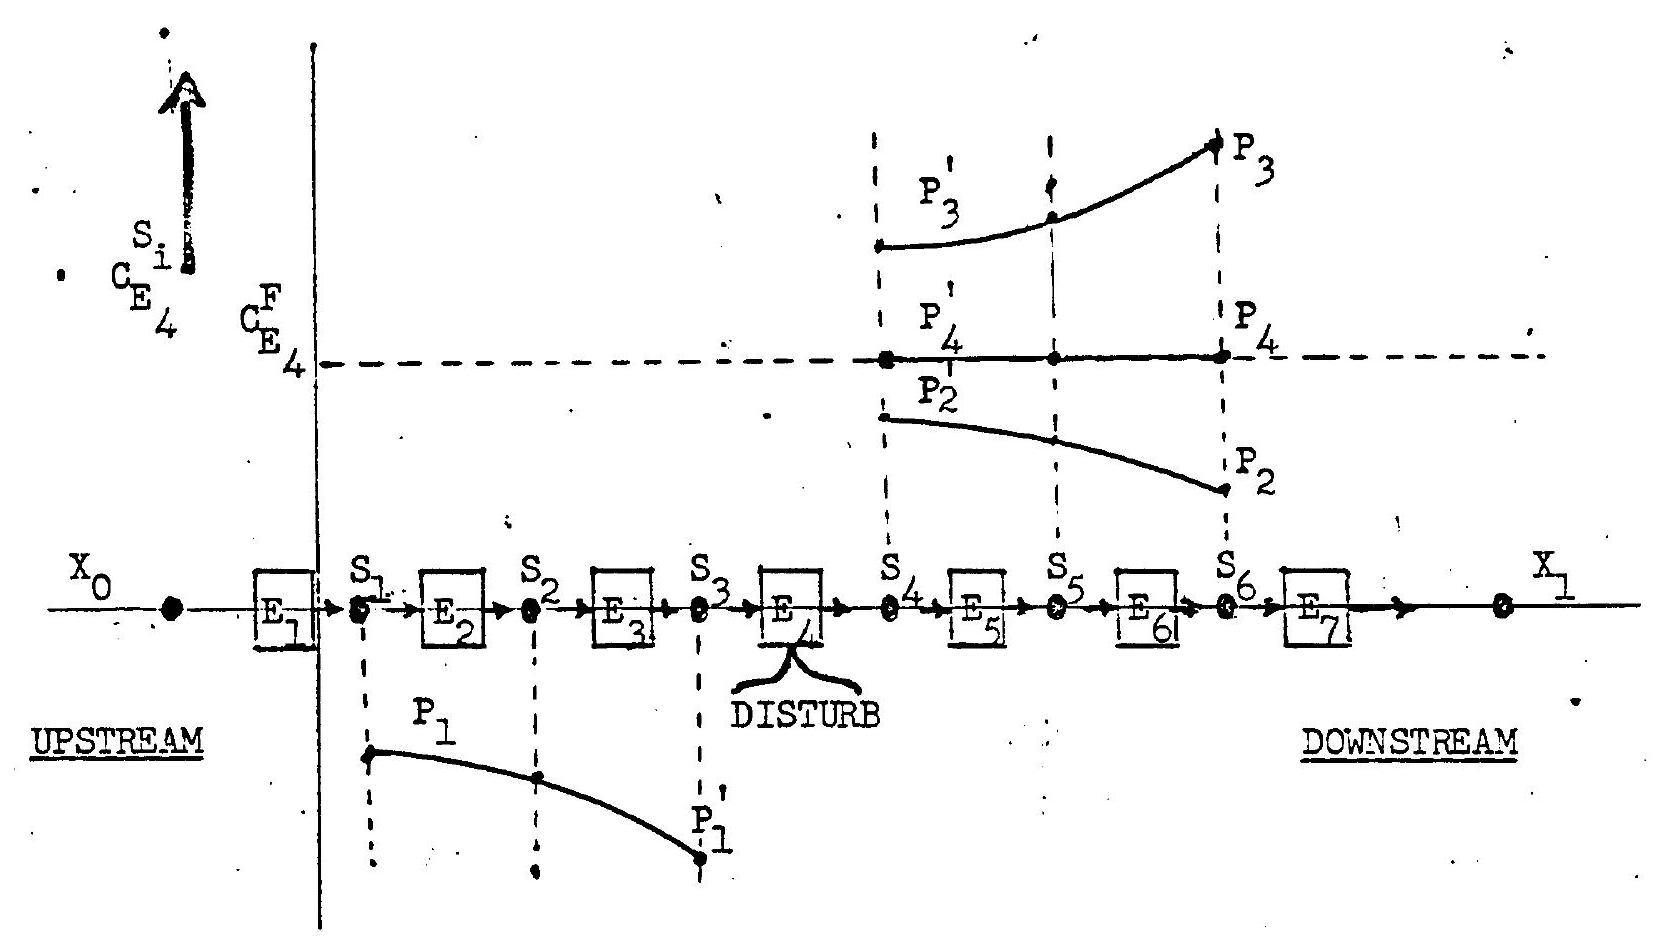
\includegraphics[max width=\textwidth]{2023_01_30_a974a42f7b7381f3f940g-150}
\end{center}

Thus, on the upstream side of the disturbance it is clear that all the $\Delta S$ must be -ve and that the effect of moving through any of the enzymes $E_{3}, E_{2}, E_{1}$ must be to `shrink' this difference from the dotted line, $C_{F}$, by the factor $A$ and then to further add the positive quantity B. $C_{F}$. Thus whatever the condition of the enzymes upstream from $E_{4}$ they will always attenuate the fractional disturbance in the pools according to a curve such as $P_{1} P_{1}^{\prime}$ on the diagram.

Downstream such a result does not necessarily apply. What actually happens will depend on the saturation and `out of equilibriumness' of the separate enzymes.

Let us suppose, for example, that enzymes $\mathrm{E}_{5}, \mathrm{E}_{6}$ are linear. In this case the factor A, for each enzyme, is of the form $\frac{S_{2}}{S_{1}}$ and the factor $B$ will be zero. Applying the relation $(3.49)$ to enzymes 6 and 5 therefore gives
%
$$
\Delta_{5}=\left(\frac{S_{6}}{S_{5}}\right) \cdot \Delta_{6}\hspace{6pt} \text { and } \hspace{6pt} \Delta_{4}=\left(\frac{S_{5}}{S_{4}}\right) \cdot \Delta_{5} \text { This shows that }
$$
%
if $C_6^{\mathrm{E_4}} < C^F_{E_4}$, that is $\Delta_{6}$ is -ve, then a curve $P_{2} P_{2}^{\prime}$ representing attenuation will be the result. If, however $C_{E_4}^{S_6} > C_{E_4}^{F}$ a curve $\mathrm{P}_{3} \mathrm{P}_{3}^{\prime}$, representing amplification of the disturbance will result, A third possibility is that $\mathrm{C}_{\mathrm{E_4}}^{\mathrm{S}_{6}} = \mathrm{C}_{E_4}^{\mathrm{F}}$ in which case the effect is to give a neutral curve $P_{4} P_4^{\prime}$ The sign of $\left(C_{E_4}^{S_6} - C_{E_4}^{F}\right)$, which determines these possibilities, depends on the condition of the last enzyme and can be considered by applying a relationship of type (3.35) to enzyme $\mathrm{E}_{7}$. This gives
%
$$
a_{7} \cdot C_{E_4}^{S_{6}} = C_{E_4}^{F}
$$
%
and hence
%
$$
C_{E_4}^{S_{6}}-C_{E_4}^{F} = C_{F}\left(\frac{1}{a}-1\right)=C_{F} \cdot Y
$$
%
where $Y$ stands for the factor $\left(\frac{1}{a}-1\right)$.

Using relationship $(3.41)$ to replace $\frac{1}{a}$ along with the inequality $1 < \beta < \frac{S_{1}}{S_{2}}$ and noting that $Y$ is a maximum when $\beta$ is a maximum we can show that
%
$$
-\frac{\mathrm{X}_{1}}{\mathrm{S}_{1}} < \mathrm{Y} < \frac{\left(\mathrm{S}_{1}-2 \mathrm{X}_{2}\right)}{\mathrm{X}_{2}}
$$
%
This result shows that whenever $S_{1}>2 X_{1}$ it is possible for $Y$ to be either negative or positive so that either an amplifying or an attenuating curve can result. The existence of the attenuating type curve, $P_{2} P_{2}^{\prime}$, or of the amplifying type, $P_{3} P_{3}^{\prime}$, depending on the degree of saturation of the last enzyme.

A further point is that if the enzymes $E_{5}$ and $E_{6}$ are not linear then there need be no steady gradient at all. However, it is never possible for $C_{E_4}^{S_i}$ to descend below $C_{E_4}^{F}$ if we start with $\mathrm{C}_{\mathrm{E_4}}^{\mathrm{S}_{6}} > \mathrm{C}_{\mathrm{E}_{4}}^{\mathrm{F}}$ and proceed in the direction $\mathrm{S}_{6}, \mathrm{S}_{5}, \mathrm{S}_{4}$.


\section{In vivo destination of elasticities}

{\bf In vivo destination of elasticities as a means of discovering the sensitivity matrix}

We return now to the idea, proposed earlier in this chapter, that it may be possible to estimable the elasticities of system components around their working position on the basis of only. a limited number of in vivo parameter modulation S.S. experiments. Having obtained estimates of these elasticities it will then be straightforward to compute the sensitivity matrix $\left[C_{\alpha_{j}}^{F, S_{i}}\right]$ using the methods already outlined.

Basically the idea is that by using our information about the `structure: of the system, that is its' metabolic diagram together with all control information, and measuring only the ratios of observed small fractional responses of type $\frac{\Delta S}{S}$ and $\frac{\Delta F}{F}$ consequent on the in modulation of only a few environmental parameters it will be possible to arrive at a complete sensitivity matrix.

Such an approach to discovering the sensitivity matrix involves no absolute measurements whatsoever, assumes nothing about the form of the rate-expression except what is implied in the structure diagram, and involves only a small number of parameter modulations which can . often be external and therefore easily manipulable. Furthermore, since the required \underline{ratios} of small fractional responses do not depend on the details of a parametric modulation but only on its location it becomes relatively straightforward to use revertants, with small but measurable effects, as a source of modulation when the structure of the system necessitates manipulation of genetic parameters.

The direct experimental methods for estimating coefficients outlined earlier, although sharing the above advantage of being in vivo and measuring only fractional responses, contrast unfavourably because they involve complicated experiments to produce exactly known modulations of genetic parameters and because it would be necessary to repeat this laborious procedure for each block in the system if we are to produce a sensitivity matrix.

Similarly the `diagnostic' approach, although perhaps useful for a quick appraisal from pool levels of possible rate controlling steps, appears even more unfavourable. Thus it involves assumptions about the form of rate-expression which are based on in vitro studies and may be of dubious relevance to the actual in vivo working of the enzyme. In addition it is difficult to determine the necessary factors to produce `scaled' pool values and the method itself is not easy to extend beyond the straight chain case just presented.

Assume then that the structure of a problem is tentatively known, that the system under study has three external pools and that a particular enzyme in it, $\mathrm{E}_{10}$, has non zero elasticity for the three pools, $S_{1}, S_{2}, S_{3}$ as shown below.

\centerline{\includegraphics[max width=0.56\textwidth]{2023_01_30_a974a42f7b7381f3f940g-154}}


Denoting the elasticities by $a, b$, and $c$ as shown and the fractional responses of $S_{1}, S_{2}, S_{3}$ and $F_{10}$ respectively by $r, s$, $t$ and $u$ and using appropriate suffixes we may consider the enzyme in isolation from the rest of the system. Using the elasticities to write down the response of the flux to variation in the pools we have:
%
\begin{equation}
\begin{aligned}
\text {For response to } & X_{1}, \quad r_{1} a + s_{1} b + t_{1} c = u_{1} \\
\text {\phantom{XXXX} " \phantom{XXXX} } & X_{2}, \quad r_{2}a + s_{2} b + t_{2} c = u_{2} \quad \\
\text {\phantom{XXXX} " \phantom{XXXX} } & X_{3}, \quad r_{3}a + s_{3}b + t_{3} c = u_{3}
\end{aligned}
\label{eqn:352}
\end{equation}
%
Provided the three response vectors $(r, s, t, u)_{1,2}, 3$ can be considered independent, which will usually be apparent from inspection of the structure diagram, the equations (3.52) will then be sufficient to determine the three elasticities.An example will make the method clear. Suppose that from general evidence the structure diagram is as below:

(Note that because of the stoichiometry there is only one independent flux, F.)

\begin{center}
\includegraphics[max width=0.9\textwidth]{2023_01_30_a974a42f7b7381f3f940g-155}
\end{center}

Suppose further that the observed fractional responses of the common flux $F$ and pools $S_{1}, \cdots, S_{6}$ to unknown but small modulation in $\mathrm{X}_{1}, \mathrm{X}_{2}$ and $\mathrm{X}_{3}$ is given in the table below.

\vspace{6pt}
\centerline{OBSERVED RESPONSE IN:}
\vspace{6pt}

MODULATE $\left\{\begin{array}{c|ccccccc|}\hline & \mathrm{F} & \mathrm{S}_{1} & \mathrm{S}_{2} & \mathrm{S}_{3} & \mathrm{S}_{4} & \mathrm{S}_{5} & \mathrm{S}_{6} \\ \hline \mathrm{X}_{2} & 0.2 & 1.8 & 1.2 & 1.0 & 0.2 & -0.6 & -0.4 \\ \hline \mathrm{X}_{2} & 0.2 & -0.2 & 0.2 & 0 & 0.2 & 0.4 & 0.6 \\ \hline \mathrm{X}_{3} & 0.15 & 0.15 & -0.6 & 0.75 & 0.15 & -0.45 & -0.3 \\ \hline\end{array}\right.$

\medskip
Using these data with the method just explained we can apply equations of type (3.52) to find that, for example, the elasticities of $\mathrm{E}_{2}$ with respect to $S_{1}, S_{6}$ and $S_{2}$ are $1, 1,-1$ respectively. For enzymes such as $E_{3}$ which have only two elasticities any two out of the three possible equations will be equivalent. Calculating all the elasticities in this way and using them to construct the sensitivity matrix we obtain

\begin{center}
\includegraphics[max width=0.9\textwidth]{2023_01_30_a974a42f7b7381f3f940g-156}
\end{center}

This result will be true even if the different pools have different `extractibilities' and it involves no knowledge of equilibrium ratios or other absolute kinetic quantities. In addition it has been obtained using data from only, three modulation experiments which themselves involve no manipulation of genetic parameters or even knowledge of the size of the modulations.

When performing the necessary modulation experiments it may happen that an X modulation which produces measurable but small responses around one enzyme will produce large changes around another. In such cases it is quite in order to obtain data for the second enzyme using a lower level of modulation, since the equations (3.52) are entirely `Local' in nature. For more complex systems having several independent fluxes it will be necessary to use the observed fractional flux responses to calculate also the stoichiometric elasticities by means of equations similar to (3.52). Inspection of the structure diagram will indicate which of these stoichiometric elasticities will be non zero for each of the enzymes. The sensitivity matrix for such a system can then be found using the additional relations (3.33) which involve the stoichiometric elasticities, the arginine cycle example given earlier illustrates this.

We wish now to consider briefly what problems might arise if the given response data were interpreted on the basis of \underline{wrong} assumptions about the stricture. In particular it is of interest to know whether such errors can be detected by analysis of the given data alone or whether further data becomes necessary.

The diagrams below show a simple example of such a situation Indicating, on the left, the `true' structure, the experimental data on which it is based and the sensitivity matrix which results. On the right of the diagram the situation is shown where the existence of the feedback inhibition is, wrongly, not taken into account and the sensitivity matrix is computed on the basis of only the $X_{1}, X_{2}$ modulation data.

%\begin{center}
%\includegraphics[max width=\textwidth]{2023_01_30_a974a42f7b7381f3f940g-158}
%\end{center}

\begin{center}
\includegraphics[max width=\textwidth]{figure3_observed.png}
\end{center}

%Calculated elasticities will be sa as for true except for enzyme $\mathrm{E}_{2} \mathrm{w}$ $\varepsilon_{3}^{2}$ is assumed to be zero and $\varepsilon_{1}^{2}, e$ are wrongly found to be $-1$ and $2.5$ respectively, instead of their real values of $1,-1$.

Inspection of the above reveals that the matrix deduced from the limited data and based upon false assumption about structure is nevertheless completely compatible with the given data. By this is meant that the 1st and 4th rows of the matrix are indeed proportional to the observed $X_1, X_2$ response vectors. However the unusual elasticities found for enzyme $\mathrm{E}_2$, which in this example are the reverse of the normal pattern of substrate activation and product inhibition, should warn the investigator that his assumptions about structure may be false. Only when further investigation has revealed the true stricture and suitable extra data has been obtained, by modulating $E_3$, can the correct matrix be found. Further consideration shows that whenever such `loops' are in fact present then the discovery of the true matrix will always involve the use of a revertant affecting an enzyme within the loop.

\section{Modulation to determine elasticities and coefficients}

{\bf Use of genetic modulation to determine elasticities and coefficients within a subsystem}

Because of the very large number of pools and enzymes in wry real biological system the experimenter will normally confine himself to observation on only a small part of it, perhaps to the values of pools ana fluxes in a few related pathways. Such a subsystem, A, together with all pools influencing it, $S_{1}, S_{2}$ and $S_{3}$ for example, is indicated below.

\begin{center}
\includegraphics[max width=0.7\textwidth]{2023_01_30_a974a42f7b7381f3f940g-160}
\end{center}

Genetic manipulation in B, possibly via the substitution of altered enzymes at $\mathrm{E}_{1}, \mathrm{E}_{2}$ or $\mathrm{E}_{3}$, can produce several independent response vectors for the pools and fluxes within and around A. How many such modulations will be actually required to estimate the elasticities of all enzymes in A depends on the structure of A. In particular if A contains loops or other complications it may in audition be necessary to use further substitutions actually within the subsystem `$A$'. Once these elasticities have been determined we can write as many 'pool'  relations of type (3.26) connecting the coefficients with respect to blocks inside $A$ as there are pools inside $A$.

However, further information will still be required since the number of blocks in A must always, exceed the number of pools by at least one. This information can be provided by direct measurement, using the methods described earlier, of one or more suitably chosen coefficients within A which can then be used together with the `pool' relations for A to determine the remaining coefficients. This approach involves the labour associated with the necessary `directly measured' coefficients but is much less laborious than direct measurement of all coefficients in A.

Alternatively if certain overall assumptions can be made about the structure of $B$ this difficulty can be completely avoided. The difference between these two methods will be made clear in the following example.

\section{Determination of $C^{F_{1} S_{i}}_{\alpha_J}$ for a system}

\subsection*{a) Making limited use of internal modulation data.}

Suppose that the complete metabolic system is shown below and let the subsystem of interest and the rest of the system be `A' and `B' respectively:

\begin{center}
\includegraphics[max width=0.8\textwidth]{2023_01_30_a974a42f7b7381f3f940g-162}
\end{center}

If no assumptions are made about the structure of $B$ then we may proceed as follows. Since no enzyme inside A has more than two elasticities, substitution of, say, $\mathrm{E}_{2}$ and $\mathrm{E}_{14}$ in $\mathrm{B}$ will provide sufficient pool and flux modulations to determine elasticities within A. These elasticities can then be used with pool relation for $S_{4}, S_{5}$ and $S_{6}$ to write down the equations connecting the six block coefficients within A. If now absolute coefficients for $E_{7}, E_{8}$ and $E_{9}$ are determined directly and the others found from them then the process will be complete.

\subsection*{b) Using only internal modulation data.}

The alternative process, which avoids the laborious direct determination of coefficients within A, involves knowledge of the structure of $B$ and is as follows. From the point of view of subsystem $A$ the details of $B$ need not be known except that it can be regarded as made up of two lumped parts $\mathrm{B}_1$ and $\mathrm{B}_2$ as shown below.

\begin{center}
\includegraphics[max width=0.9\textwidth]{figure3_bInternal.png}%2023_01_30_a974a42f7b7381f3f940g-163}
\end{center}

As before all elasticities within A can be found by substitution in $B_{1}$ and $B_{2}$ and in addition the effective elasticity `a' of the subsystem $B_{1}$ with respect to $S_{2}$. Finally the same substitution in $B_{1}$ together with two more made within $A$, say at $E_{8}$ and $E_{9}$, will together provide sufficient date to determine the elasticities, $(b, c$ and $d)$ of the lumped block $B_{2}$. From these elasticities and the simplified structure the true absolute coefficients within A may be determined. Thus, provided the structural assumptions are correct, the experimental effort is just that of determining pool and flux responses for the subsystem A for four substitutions about which nothing need be known except that their effects be not too large.

This latter approach involves exploiting to the full all structural knowledge of the larger metabolic system which will have been gained by a variety of qualitative methods over many years. It seems to offer the best hope of making a `quantitative' estimate of the relative importance of different transformational steps, or blocks, since it builds effectively on existing qualitative information and involves only a minimum of quantitative data which need not involve any absolute measurements. The difficulties in the method arise mainly from the difficulty in determining with reasonable accuracy the small fractional changes in pools and fluxes which are needed and this will be particularly severe in the case of flux determinations.

\section{Optimal allocation for growth}

At the end of CHI.II it was shown that a fairly general model giving the S.S. of a `complete' growing system was defined by the form% determination of coefficients within A, involves knowledge of the structure of $B$ and is as follows. From the point of view of subsystem $A$ the details of $B$ need not be known except that it can be regarded as made up of two lumped parts $\mathrm{B}_1$ and $\mathrm{B}_2$ as shown below.
%
$$ \sum \lambda_{ij} g_j f_j(\olsi{S})-\frac{g_0}{\sum g_j} \cdot g_p \cdot k \cdot f_p(\olsi{S}) \cdot \olsi{S}_i=0 $$
%
The growth rate, $G$, being given by the measure:
%
$$G=\dfrac{g_{p} f_{p}(\olsi{S})}{\sum_{g_j}}. $$
%
We now wish to consider, for a system where the $g^{\prime}s$ are given as parameters, what configuration of the allocation vector $\left[g_{1}, g_{2}, \cdots\right]$ will maximise $t$ growth rate.

Provided the allocation to structure is small compared with that to active protein $\frac{g_{0}}{\Sigma g_{j}}$ will be small and it is possible to treat the problem in a simple way. Thus under these circumstances the problem becomes identical to one where the $\mathrm{E}_{j}$ are given as parameters and the S.S. is defined by
%
$$
\sum \lambda_{ij} E_{j} f_{j}(\olsi{S}) = 0
$$
%
The aim being to maximise the growth rate, $G=\frac{E_{p} f_{p}(\olsi{S})}{\sum E_j} = \frac{F_P}{\sum E_j}$ by adjusting the different enzymes. This can be done by adjusting only the \underline{ratio} of the enzymes whilst keeping their sum constant, since it is only the ratio of the enzymes which affects G. When the optimal allocation exists a small change in the ratio of any two enzymes such that the sum remains constant will have no effect on the flux to protein $F_{p}$ Thus if an amount $\Delta \mathrm{E}$ is transferred from $E_{k}$ to $E_{j}$ around this optimum condition we must have
%
$$
\frac{\Delta F_P}{F_P} = 0 = C_{\alpha_{j}}^{F_P} \frac{\Delta E}{E_{j}} - C_{\alpha_{k}}^{F_P} \cdot \frac{\Delta E}{E_{k}}
$$
%
So that, when optimal allocation exists, we have for any two enzymes $j$ and $k$
%
\begin{equation}
E_{j} : E_{k} = C_{\alpha_{j}}^{F_P} : C_{\alpha_{k}}^{F_P}
\label{eqn:353}
\end{equation}

What this pattern of coefficients and enzyme concentrations actually turns out to be will of course depend on the details of the separate enzymic proteins and the network in which they are embedded. If one of them, for example, has a very low turnover number it will, even at its optimal allocation, require a large amount of protein and have a large coefficient. The following example will make this clear.

\section{Straight chain of linear enzymes}

Consider the chain of enzymes shown below, where $\mathrm{X}$ is the initial substrate and the final reaction is irreversible. The activity, of the separate enzymes is now given as the product, $E_{i} \cdot t_{i}$, of enzyme quanti ty and turnover number

\begin{center}
\includegraphics[max width=\textwidth]{2023_01_30_a974a42f7b7381f3f940g-166}
\end{center}

Provided the pools are scaled so that all equilibrium constants are effectively unity the relations (1.18) and (1.19) of CH.I giving the flux and the $C_{\alpha_{1}}^{F}$ can be written as follows. Thus
%
\begin{equation}
F=\frac{X}{\sum \frac{1}{V_{i}}} = \frac{X}{\sum \frac{1}{E_i \cdot t_{i}}}
\label{eqn:354}
\end{equation}
%
and
%
\begin{equation}
C_{\alpha_{i}}^{F} = a \cdot \frac{1}{V_{i}} = a \cdot \frac{1}{E_{i} \cdot {t_i}}
\label{eqn:355}
\end{equation}
%
Where $a$ is the same constant for all enzymes.

We can now apply the relation (3.53) in order to discover the optimal allocation of enzymes which will maximise $F$ for a given total enzyme $E_{T}$ and ensure the maximum growth rate.

Thus $(3.53)$ can be written as
%
$$
E_{i}=b \cdot C_{\alpha_{1}}^{F} \text { where } b \text { is the same constant for all enzymes }
$$
%
and combined with the expression (3.55) for the coefficients this gives
%
$$
E_{i}=b_{\cdot} C_{\alpha_{i}}^{F} = a \cdot b \cdot \frac{1}{E_{i} t_{i}}
$$
%
or
%
$$
E_{i} \propto \frac{1}{\sqrt{t_{i}}}
$$
%
Hence we have that the optimal allocation of enzymes in the chain is such that
%
\begin{equation}
E_{1}: E_{2}: E_{3}: \cdots=\frac{1}{\sqrt{t_{1}}}: \frac{1}{\sqrt{t_{2}}}: \frac{1}{\sqrt{t_{3}}}:
\label{eqn:356}
\end{equation}
%
To find the corresponding maximum growth rate we must use this enzyme ratio in (3.54) to give $F_{\max}$ for a given $E_{T}$ Thus from (3.56) we have
%
$$
E_{i} = E_{T} \frac{\frac{1}{\sqrt{t_{i}}}}{\sum \frac{1}{\sqrt{t_{i}}}}
$$
%
and $\dfrac{1}{E_{i} \cdot t_{i}} = \dfrac{\sum \dfrac{1}{\sqrt{t_{i}}}}{E_{T} \sqrt{t_{i}}}$. Putting this into (3.54) we now get
%
$$
F_{\max} = \frac{X_{\cdot} E_{T}}{\left(\sum \frac{1}{t_{i}}\right)^{2}}
$$
%
So that the maximum growth rate is
%
\begin{equation}
\mathrm{G}_{\max } = \frac{F_{\max}}{E_{T}} = \frac{X}{\left(\sum \frac{1}{\sqrt{t_{i}}}\right)^{2}}
\label{eqn:357}
\end{equation}
%
In particular suppose that the chain consisted of three enzymes having turnover numbers of 1, 4 and 9 respectively and that $X=1$ and $E_{T}=9$. If the enzymes are allocated equally the growth rate is given by calculating $\frac{F}{E_{T}}$ using $(3.54)$ giving
%
$$
G=\frac{1}{9} \cdot \frac{1}{\frac{1}{3}+\frac{1}{3 \times 4}+\frac{1}{3 \times 9}} \quad=0.25
$$
%
on the other hand $G_{\max}$ for optimal allocation is given by (3.57) as
%
$$
G_{\max } \bumpeq \frac{1}{\left(1+\frac{1}{2}+\frac{1}{3}\right)^{2}} = 0.3
$$
%
In this case optimal allocation of the enzyme has only improved the growth rate by approximately $20 \%$ from that obtained with an equal allocation.

\section{Optimal solution given alternative food sources}

Consider the three linear enzymes shown below.

\begin{center}
\includegraphics[max width=0.5\textwidth]{2023_01_30_a974a42f7b7381f3f940g-168}
\end{center}

In this case, if we consider $\mathrm{F}_{3}$ as the flux to protein, the problem is to find the best allocation between $\mathrm{E}_{1}, \mathrm{E}_{2}$ and $\mathrm{E}_{3}$ It can be shown by a simple argument that the maximum must be one or other of the solutions in which either $\mathrm{E}_{1}$ or $\mathrm{E}_{2}$ is zero. Using the previous example this gives the maximum as being the greeter of the two expressions
%
$$
\frac{X_{1}}{\left(\frac{1}{t_{1}}+\frac{1}{t_{3}}\right)^{2}} \quad\text{ and }\quad \frac{X_{2}}{\left(\frac{1}{t_{2}}+\frac{1}{t_{3}}\right)^{2}}
$$
%
This means that, depending on the ratio of $X_{1}/X_{2}$, the optimal organism of this type will choose to feed exclusively on one or other of the alternative nutrients but never on both.

\subsection*{Role of regulation}

It seems clear that for organisms such as E.coli where growth rate is of great selective value, an important role for the regulatory loops found may be to adjust the enzyme allocation so that it approximates to optimal over a variety of environmental situations.

In computer studies it will be of interest to introduce suitable regulatory functions for the $g_{i}$, which can respond to both $X$ and $S$ values, and to compare the allocations achieved by such systems with the computed optimal allocations over a range of environmental situations. Such studies could give us some quantitative idea of the value, from the point of view of maintaining a high growth rate, of the various regulatory mechanisms found. 


\chapter{Computer Methods For Studying The Steady State Behaviour Of Theoretical}
\markboth{COMPUTER METHODS}{}

\section{Multi-Enzyme systems}

In this chapter a brief account will be given of computer methods which have been developed in order to facilitate the study by numerical solution of the otherwise intractable sets of simultaneous non-linear algebraic equations which define the stationary solutions of a multi-enzyme system.

In developing suitable methods two general aspects of such a study were considered particularly important. Firstly that the type of study which we have in mind is always experimental in nature, being in fact an experiment `in numero' on a theoretical system rather than, say, an experiment 'in vitro' on a reconstructed system, Because of this it is important that the computer methods used should allow the experimenter great flexibility in varying the values of parameters, in altering the actual structure of the system under consideration and in deciding what `measures' are to be made on the system. Ideally this flexibility will be achieved by having the experimenter `on line' to the computer and able to communicate with it in some sort of `biochemical language' which is simple to learn and use, and will allow him both to specify the metabolic system and to subsequently perform experiments on it. In practice any computer methods developed should be capable of evolving towards this ideal as `on-line' facilities become widely available.

The second aspect of importance is that the demands which such `in numero' experiments place on the available computer resources should not be so large that the user obtains only a poor response from the computing service, For our own purposes it was thought that the computer methods chosen should be able to perform a significant set of in numero experiments, say 100 S.S. and sensitivity matrix determinations on a medium sized system of 20 non linear enzymes, within a resource allocation which could be available to an average user on at least a daily basis.,
Keeping these requirements in mind the first decision is whether to employ an analogue or a digital computer.

\section{The Analogue computer}

For simulation work the analogue computer has two main advantages. Firstly that the analogue components, when suitably interconnected for a particular study, correspond directly to the `blocks' of the system being simulated and secondly that voltages on the components are directly representative of system variables. Secondly there is the ability to `interact' directly with the system by, for example, adjusting parameter(s) which correspond to potentiometer settings and then observing the response of system variables, often by direct oscilloscope display.

These advantages largely meet the requirement to be `onIine' and to have a simple means of carrying out, experiments on the system. However, the task of specifying the system in a form suitable to the analogue computer may still be formidable.

On the other hand the analogue computer has numerous disadvantages. Thus the size and non-linearity of, systems which can be simulated on any given computer is usually severely limited by the number of analogue components available and, furthermore, to avoid serious inaccuracy, system variables have to be `amplitude scaled' so that voltages lie within a limited range. Often repeated `rescaling' of a problem is necessary as an experiment is conducted. In addition there is always difficulty in repeating `runs' since analogue components are constantly developing minor faults.

For our own requirements the disadvantages just noted considerably outweigh the possible advantages, Thus ruling out the use of analogue computers for all but the smallest problems. For example, even with the quite large analogue computer available to us we would have been limited to the equivalent of about 7 nonlinear unimolecular enzymes with the further limitation that it would not have been easy to produce conveniently even an approximation to a sensitivity matrix.

\section{Digital computer systems}

By comparison the digital computer, if it is working at all, is highly accurate and completely reliable, usually being maintained by a service organisation. Furthermore there is, within reason, no limit to the size and non-linearity of the system being simulated except that the larger metabolic systems will require more time. In practice a further important advantage of digital machines is that, for mainly commercial reasons, far more effort is being devoted to * their development than is to that of analogue machines, so that each year they become more powerful and more widely available.

In recent years a large number of `simulation languages' have been written in which the general aim is to retain the undoubted advantages of the analogue computer whilst actually using a digital by machine, a useful review of some of these languages is by R.D. Brennan, (1964). In general these languages have been successful in allowing the user to work in terms of the `block' structure of his problem and in allowing him to easily load the structure and initialise the values of parameters. However, they have been less successful in allowing the user to `interact' with his system, since the proper development of such interaction must await the general availability of `conversational' operating systems at computing centres.

In order to discuss the particular methods which have here been used in devising a suitable 'simulation language' for the steady state properties of multi-enzyme systems. it will be necessary to give a brief description of certain concepts and terms commonly employed in digital computer science.

A computer system is indicated in the diagram below in which all details other than those required for a general understanding have been omitted

\includegraphics[max width=0.9\textwidth]{figure4_cpu}

The C.P.U. or `Central Processing Unit' is capable of reading binary stored patterns stored in locations within the high speed magnetic core store, and interpreting these patterns as 'instructions' which will control the next action of the C.P.U. When an instruction has been completed the C.P.U. will automatically fetch the next one from a designated location.

A modern machine will be capable of distinguishing and executing about one hundred distinct binary patterns as `legitimate' instructions each of which causes the C.P. U. to carry out a specific basic operation. These include `data transfer' instructions which move binary patterns, now considered as data, between registers in the C.P.U. and other registers, either in the core store or associated with various input, output, or mass storage devices. Input devices include teletypes, card and paper. punches, graph plotters, line printers and mass storage, includes magnetic tape, magnetic disc, magnetic drum etc. Other `data manipulation' instructions are concerned with carrying out operations on designated bit patterns, usually held in one or more registers belonging to the C.P.U, these include for example, arithmetic operations such as multiply and divide, logical operations such as `AND'ing two bit patterns etc. Usually the C.P.U. will fetch and execute instructions which lie sequentially in core, but certain instructions can determine from which core location the next instruction is to be fetched, so that, for example, it is possible to repeat a sequence of instructions until some condition is satisfied before continuing with further instructions.

A set of such instructions in core is called a `binary program' and, starting from a given instruction, will cause the C.P.U. to carry out a complete sequence of operations. For example it might read in a set of numbers, previously punched on paper tape and fed to a tape reader, store them as `data' in core, proceed to find their mean value and standard deviation and output the results on a line printer before returning to the start of the program ready to read in further input from the tape reader.

A modern computing system will provide a number of special. `system programs' which greatly simplify the task of the user and also help to ensure that the computer is being efficiently used.

One type of system program is an `operating system' or `O.S.' which has the important task of supervising the activities of all other programs (sequences of instruction in core, or on backing store) which are current. Thus if there are several programs in core at any one time a `multiprogramming' O.S. will allocate C.P.U. time to each in turn and will ensure that their input and output is connected with the appropriate peripherals. Or again the O.S. may maintain a `queue' of programs on a disc, so that the C.P.U. never runs out of work, and arrange for programs to be moved from and to backing store so that valuable core space is not wasted on inactive programs. An important goal for advanced O.S. is to allow a user to work from his own input/output station, just as if the computer were dedicated to him alone, this effect being achieved by the O.S `time sharing' the C.P.U. and other system resources amongst users active at any moment. This will eventually be important for simulation work (D. Garfinkel et al., 1970) since it will then be possible to `interact' with the system under study. Unfortunately such `conversational' O.S. have not proved easy to implement in any efficient way and are only now becoming available to the ordinary user in the U.K.

Another type of system program is a `compiler' which has the task of translating a program written in a `high level' source language into an equivalent binary program suitable for running on a particular machine. This relieves the user of the impossibly tedious task of breaking his problem down to the level of a series of binary coded machine instructions and instead allows him, to concentrate on describing his problem in one of the more or less readable high level languages. These include the well known `ALGOL' (ALGOrithmic Language) and `FORTRAN' (FORmula TRANslation) languages: compilers are available on most large machines to translate source programs, written in these languages into the equivalent binary code.

With the reasonably advanced O.S. presently available the user can call, by means of `control statements' which inform the O.S. of his wishes, any stored binary program such as a compiler and feed data to it from any specified input. This allows him for example to call further binary programs: which will receive as data the output of previous programs. If the O.S. provides conversational facilities he will in addition be able to interact with appropriately written programs. For example with a conversational 'editor program' or perhaps with his own suitably written simulation program.

\section{Design of suitable simulation system}

The actual implementation of a simulation system which broadly meets the requirements set forth at the beginning of this Chapter will depend very mach on the general facilities provided by the local computing centre. In our own case the situation was that the centre provided a reasonably advanced but non conversational 0.S. together with the `ALGOL' type of language compiler considered capable of producing nearly optimal binary code. With regard to `computing power' rough estimates indicated that the `KDF 9' computer, available at the time under this system, would, if carefully programmed, take about 10 minutes to complete the daily simulation work. Neither the limited basic computing power available to us nor the lack of a 'conversational' mode was thought likely to change appreciably for some years.

In these circumstances the basic decision was taken that the `structural input' for a simulation, that is the data which specifies the rate expression and how they are interconnected to give the functions, $\phi_{i}(S, P)$, would have to be converted by the available.

compiler into efficient binary code for evaluating the $\phi_{i}$. This was thought necessary because the `heart' of a simulation involves repeated numerical evaluation of the $\phi_{i}$ and any gain in efficiency at this level will immediately be reflected in the performance of the simulation program. A number of earlier simulation programs have not attempted to produce efficient code in this way and were correspondingly slow, thus limiting their usefulness. For example the earlier programs of Garfinkel were of this so called interpretative type (D. Garfinkel et al., 1970), which in effect meant that each evaluation of the $\phi_{1}$ involved the unnecessary work of rescanning a stored interconnection matrix, a step which in our method would be carried out only once at the compiling phase. G.H. BURGIN, (1966), who converted his originally interpretative `MIDAS' program so as to include a compilation phase claims an increase in `speed' of between 5 and 10 fold over the old version.

Since the `structural input' would not conveniently be in a form suitable for compilation it was decided to feed it as data to a program written by ourselves and designated the `precompiler'. The purpose of this `precompiler' was to convert the incoming structural data into a high level language and combine it with existing code to form a 'simulation program' suitable for passing on to the compiler. It was further decided that'this simulation program should, after compilation, be itself capable of receiving `commands' in a simulation language so that the user would not lose any of the advantages of purely interpretative simulation systems which usually provide a flexible means of controlling the actual simulation ``running phase''.

The use of a `precompiler' phase to construct and present for compilation a simulation program which can itself be driven by its own simulation language is shown in the figure opposite, and this general design has several results. Firstly it avoids the `inefficiency' disadvantages of a purely interpretative system since it ensures that basic and time consuming operations such as evaluation of the $\phi_{i}$, solution of differential equations and inversion of matrices will be in the form of nearly optimal binary code. Secondly it separates simulation into the two distinct phases of 'loading' and 'running' as indicated in the figure. This separation has the advantage that once a structure has been loaded it may be repeatedly investigated by supplying data, in the form of commands in the simulation language, to 2 stored binary version of the simulation program there being no need to return to the precompiler-compiler level unless it becomes necessary to alter the structure. Thirdly, it will be possible, depending on the sophistication of the precompiler and simulation program, for a user who is unfamiliar with programming to load his enzyme network using a notation which involves only simple algebraic and biochemical concepts and run his experiments by means of a series of simple `commands' interspersed with the necessary data. This will have the important effect of putting the power of the computing system directly into the hands of the investigator concerned. A further advantage in this respect is that although the main features of the simulation 'command' language are fixed it becomes a simple matter using the precompiler to add new commands as and when they are needed.

\includegraphics[max width=0.9\textwidth]{figure3_3.png}

Finally the production of the simulation program via a precompiler stage and its command language running technique are well suited for its efficient operation under conversational O.S. as they become available and little reprogramming will be necessary. In this respect the precompiler stage should result in a simulation program of high efficiency and with minimum demands on core storage Both of which are essential attributes if a reasonable response is to be obtained from the conversational 0.s. of the near future which will impose a heavy penalty on programs making large demands on time and core. The advantages of a `fast' simulation program are also very relevant to the `archive' problem. Thus the experiments to which we have referred consist in moving through `parameter-space' and observing the response of all system measures of interest. If the computation of the S.S. were very expensive in computer time it would become necessary to file or `archive' the results of experiments in case they were needed again for comparison with the results of later experiments as indeed they often would be. Such a strategy is, however, hardly practical on account of the difficulty of devising a filing system which could cope with the continuously expanding exploration of a virtually infinite parameter space, both from the point of view of classification and because of the sheer bulk of information. If, however, the computation of the S.S. is sufficiently fast no such problem need arise since it will be possible to recompute the same S.S. whenever it is required for purposes of comparison.

\section{Implementation on the KDF 9}

A simulation system of the general design just outlined was implemented on the Edinburgh University KDF 9 computer during 1968, several earlier versions having been discarded, and demonstrated at the FEBS summer school on `Computing Techniques in Biochemistry' in the same year. General impressions of my own and other, simulation programs are set forth by J.G. Reich, 1969.

In view of the impending removal of the KDF9 and also of proposed modifications to the high level language it was decided to keep the implementation as simple as possible within the general framework of having a `precompiler' and a 'simulation program'. With this in mind the 'biochemical language' was, for the meantime, taken as an algebraic specification of the rate-expression and of their use in forming the $\phi_{i}$ whilst the simulation language was restricted to being entirely numerical, with -ve numbers representing the various commands and +ve numbers the corresponding data. Both of these restrictions could of course be lifted in fuṭure versions of the simulation system, their purpose being merely to facilitate the first version. Thus the restricted biochemical language was suitable for direct compilation by the available compiler (Atlas Autocode). Whilst the precompiler, having no need to transform the incoming data, assumed more the form of an EDITOR which would edit the incoming text into the text of a previously filed simulation program. The editing aspects of the precompiler in fact proved so useful to myself and others that a `public' version, produced in collaboration with Dr. J.G. Burns of Edinburgh University, was made available to other users of the computing centre. A users guide to this is provided in the appendix.

\section{Editor (precompiler)}

This will not be described in detail since it is marginal to the enzyme simulation problem however its main features will be outlined since any future precompiler would almost certainly include them. The user operated the editor by means of issuing 'commands' which were followed, as appropriate, by the names of text files to be manipulated, line no's to be edited within the files and sections of text to be inserted. The basic operation of the editor was to take the text from a magnetic tape file, place it in core and edit it in accordance with the commands `DELETE', `INSERT' and `ALTER'. The resulting text could be passed to the compiler, by means of the command `RUN', for conversion into an equivalent binary program whilst the old version of the text on magnetic tape would automatically be overwritten by the new one unless the command `NOWRIT' was used. In addition text could be moved from one file to another by means of the command `BRANCH', inserted direct into a file from an input device by means of the command `FILE' or stored and retrieved from a `library' by means of special library commands. The editing system in its final form worked off one magnetic tape and maintained six text files each capable of holding a large program as well as a sizeable library.

In retrospect the editor turned out to be an essential part of the complete simulation system. Thus whilst enabling the non-programmer to 'load' the system using a standard sequence of editing instructions it also allowed the more sophisticated user to carry out the following operations.

i) Retain `on file' the text of all `networks' of interest. So that they could be modified when required, using the editor, and the new simulation program automatically established.

ii) Extend the simulation program itself by adding new routines and by developing special versions to study particular problems.

iii) Correct faults which from time to time were discovered in the simulation program.

It may be argued that the functions of the editor amounted to no more than `shuffling cards' or, as was the case at that time, editing paper tape. In practice, however, the ability to store, edit and list several large programs places the user in an altogether different position and makes feasible the type of activity which is essential to simulation. It turned out also that the programming techniques involved in writing the editor were very similar to those required for a simulation program capable of receiving a simple command language. In each case it is necessary to read in commands, look them up in a dictionary and then, using a `switch', select an appropriate sequence of routine calls which will carry out the command returning to read in the next command when execution is complete.

\section{The simulation language}

As mentioned earlier this was kept as simple as possible, being entirely numeric, both to reduce the size and complexity of the simulation program and also to keep the `commands' as concise as was possible. The integer part of each -ve number in the input stream will select a command and the first two decimal digits the particular `type' of that command if alternatives exist. A table of `commands' is shown opposite and an example of their use will be given in the next section. The main features of this table are as follows.

\subsection*{I. Selection of network}

If several networks have been previously loaded and the binary version of their corresponding simulation programs stored on magnetic tape it is possible to select among them using the command of type \kcmd{-0.XX}.

For example the command \kcmd{-0.02} means that the simulation program for a particular network which was previously compiled and filed in binary form in file number 2 is to receive any subsequent commands. If after some time it wished, say, to investigate the network held in file number 1 it is necessary for operations in file 2 to be brought to a close by means of the command \kcmd{-0.99} and the new system can be selected by means of the command \kcmd{-0.01}.

\begin{figure}
\includegraphics[max width=0.9\textwidth]{2023_01_30_a974a42f7b7381f3f940g-186}
\end{figure}

\subsection*{II. Parameter modification}

Parameters embedded within the expressions defining the $\phi_{i}$ can be altered in two ways, either by multiplying them by a specified factor or by replacing them with a new value.

Multiplication and replacement are brought about respectively by the commands \kcmd{-3.XX} and \kcmd{-4.XX} where \kcmd{.XX} specifies the particular type of parameter being modified as indicated in the table. For example the command \kcmd{-3.02} indicates that we wish to alter the quantity of an enzyme by multiplying its present quantity by some factor. Commands of this type must of course be accompanied by the appropriate `data' in the form of a set of +ve numbers preceding the command and provision is made for the user to provide as many pairs of numbers as required each pair specifying the enzyme to be changed and the amount by which it is to be multiplied respectively. For example the line

$11\qquad 10\qquad 4\qquad 5.2\qquad -4.02$

causes the operations $e_{1}=e_{1} \times 10 \mbox{ and } e_{4}=e_{4} \times 5.2$ to be carried out, where $e_{1}$ and $e_{4}$ represent enzyme quantities.

\subsection*{III. Output of the values of parameters and variables and printing of `messages'}

Output of values can be achieved by means of the command \kcmd{-5.XX} where the \kcmd{X} again selects the parameter or variable type which it is required to output. In this case the command always outputs the values of all members of a given parameter type and there is no need for precedent data. For example if there were 10 pools in a given system the command \kcmd{5.06} would cause the values of $S_{1}, S_{2}, \cdots S_{10}$ to be printed out, in that order. For convenience the command \kcmd{-5.00} causes a complete output, being equivalent to \kcmd{-5.01}, \kcmd{-5.02} $\ldots$ \kcmd{-5.08}. In order to improve the legibility of the output the command \kcmd{-7} can be \underline{followed} by any `message', the effect being cancelled when the end of the line is reached.

\subsection*{IV. Selection of sensitivity coefficients for subsequent output.}

Commands of the type {\tt \textquotesingle -6.XX'} will select which parameters the coefficients are to be found with respect to. Thus whenever a S.S. is subsequently computed only selected rows of the generalised sensitivity matrix $\left[C_{P_j}^{S_{i}, F_j, M_{K}}\right]$ will be outputted. In this case, the \kcmd{.XX} specifies the type of parameter, $P, X$, etc, and a list of the +ve numbers preceding the command specifies which members of the type vector, $X_{1}, X_{2}$ etc, are required. For example the two command lines,

$\begin{array}{llll}1 & 5 & 7 & -6.01 \\ 4 & & &-6.05\end{array}$

will select for subsequent output the rows with respect to $P_{1}, P_{5}, P_{7}$ and $X_{4}$ respectively. The command {\tt -6.00} will select \underline{all} rows of type $C_{\alpha i} $ i.e. the block coefficients, and requires no precedent data.

\subsection*{V. Storage and Retrieval of Values}

Often it is convenient, after a sequence of parameter variations for example, to, return to an earlier set of parameter and variable values. There are several commands which are of use in this situation. Thus \kcmd{-1} will `shunt' the existing values of all parameters, variables, matrix elements etc. onto magnetic tape and \kcmd{-2} will `recover' them. The commands \kcmd{-8.XX} and \kcmd{-9.XX} perform a similar function but are more limited, the \kcmd{.XX} referring to manipulation of either the pool or the enzyme quantity vectors by themselves. For example the command \kcmd{-8.01} will store the existing enzyme values and the command \kcmd{-9.01} issued subsequently will then overwrite any new enzyme vector which may have arisen with the original one which was stored.

\subsection*{VI. Computation and output of S.S.}

A number of commands are concerned with causing S.S. calculations to be performed and also with outputting the results. Thus \kcmd{-1}, which can be called after any parameter adjustments, will cause variables to move to their S.S. values and will automatically output all pools, fluxes, special measures and any coefficients which have been selected.

If it is required to compute and output a sequence of S.S.solutions corresponding to a steadily increasing value of some parameter this can be achieved concisely by means of the `SPREAD' command of type \kcmd{-12.XX}. For example the line

{\tt \textquotesingle 1010203 \qquad  3 \qquad 2 \qquad 3 \qquad -12.03\textquotesingle}

will cause $\mathrm{X}_{3}, \mathrm{X}_{2}$ and $\mathrm{X}_{1}$ specified in the leading `KEYWORD', each to be modulated up and down by three powers of 2, thus computing 9 S.S. around the original position.

\subsection*{VII. Adjustment of enzymes to achieve a given S.S.}

A further useful command is \kcmd{-10} or `FLOAT' which, when supplied with precedent data for all pools and `independent fluxes' will adjust or `float' the values of the enzymes carrying 'dependent' fluxes so that a perfect steady state is achieved corresponding to these specified pools and independent fluxes. Since one may often wish to model a situation where relative fluxes and pools are roughly known this command has proved useful.

\section{Loading and running a system}

To make clear the steps which are involved in using the simulation system we will consider the six enzyme divided pathway network shown below:

\begin{center}
\includegraphics[max width=0.75\textwidth]{2023_01_30_a974a42f7b7381f3f940g-191}
\end{center}

The network involves a metabolic inhibition $i_1$, and as an example, is supposed to be a subsystem in an expanding space which has an exponential growth constant $P_{1}$

\section{Loading}

Below are set out the main stages involved in loading the system via the precompiler. The notation used is similar, but not identical, to that actually used on the computer, and corresponds to the notation of CM.I and II. The input is typed onto paper tape or cards or, if an on-line system is available, perhaps direct into the computer. The precompiler stage can detect certain `obvious' errors in the input and `abort' the loading phase, if these are sufficiently severe.

\section{Details of step}

{\renewcommand{\arraystretch}{2}
\begin{tabular}{lp{10cm}}
STEP & DETAILS OF STEP \\ \\
A & Provide correct control. statements to activate the EDITOR/
precompiler and find the relevant text for the required
simulation program from among the editors files. \\
%
B &
Type out the six flux expressions giving the flux at each of the six blocks in terms of the surrounding pools etc. Thus

$F_{1}=E_{1} t_{1}\left(X_{1}-S_{1} / K_{1}\right) \times i\left(1, S_{3}\right)$

$ F_{2} = E_{2} t_{2}\left(S_{1}- S_{2} / K_{2}\right) / \left(1 + S_{1} / P_{2}+ S_{2} / P_{3}\right)$

etc \\
%
C &
Show how the 'Fs' combine to produce the pool rates of change, including the effects of expansion. Thus

$\phi_{1}=F_{1}-F_{2}-P_{1} S_{1}$

$\phi_{2}=F_{2}-F_{3}-P_{1} S_{2}$

etc \\
D &
Taking the two independent fluxes as the outputs $F_{4} F_{6}$ show how the dependant fluxes are related to them

$\mathrm{F}_{3}=\mathrm{F}_{4}+\mathrm{P}_{1} \mathrm{S}_{3}$

$\mathrm{F}_{5}=\mathrm{F}_{6}+\mathrm{P}_{1} \mathrm{S}_{4}$

$F_{2}=F_{3}+F_{5}+P_{1} S_{2}$

etc \\
%
E &
Write down expressions defining any special `measures'
which are currently of interest. For example the ratio
of fluxes in the two pathways
%
$$ M_{1}=\frac{F^{4}}{F_{6}} $$ \\
%
F &
Assign values to all parameters and I.C. to pool
variables any not assigned will automatically have
value unity. Indicate which binary file should hold
the compiled version of the simulation program

$ \mathrm{P}_{1}=0.001 $

$ \mathrm{P}_{2}=10 $ \\
%
G &
Provide a title for the network, which will be automatically printed out whenever it is run. Thus
`SIX ENZYME DIVIDED RATHWAY WITH INHIBITION' \\
%
H &
Provide, in high level programming language, the code necessary to execute any special commands which you wish to add to the basic simulation language for this investigation, these to be numbered from 20 upwards. Thus

$ 20: \ldots\ldots $

$ 21: \ldots\ldots $
\end{tabular}}

In principle sections $C$ and $D$ could be omitted since they duplicate information already contained with the rate expressions of B.

However they do not represent a large amount of input and they have been included rather than employing a more complex form of precompiler. The representation of inhibition is simplified by means of a standard inhibition routine $i(S, n)$ available within the standard simulation program. Any number of functions can be set up in this way, each being defined by four parameters which control its' slope, maximum inhibition, etc. and which can themselves be modified via the simulation language.

When all sections have been loaded the precompiler incorporates them into the text of the standard simulation program held in its files and feeds the resulting complete program to the compiler. If the program compiles successfully, that is has no obvious errors in it, the resulting binary version will be placed into the designated binary file where it can be repeatedly accessed for use in the 'run' phase by the appropriate {\tt -0.XX} command.

\section{Running}

The system just loaded can now be accessed for experimentation indefinitely unless it is required to alter its structure or perhaps add some extra 'commands'. The following sequence of commands exemplifies one such experiment.

\begin{center}
\includegraphics[max width=0.95\textwidth]{2023_01_30_a974a42f7b7381f3f940g-195}
\end{center}

The above experiment is intended to see what effect the presence of the inhibition $i_1$ has on the pattern of sensitivity coefficients for increasing levels of $X_1$

\section{The simulation program}

Here it seems useful to outline certain aspects of the program these being concerned broadly with the `numerical' techniques for locating the S.S. and the programming techniques for interpreting the simulation language. The overall program consists in declaring `arrays' for all the variable types involved, such as $\mathrm{E}, \mathrm{t}$ and $\mathrm{p}$, the size of these arrays being filled in by the precompiler at `load' time. Space is also declared for the matrix $\left[\frac{d \phi_{i}}{d S_{j}}\right]$ which is required. for the iteration procedure mentioned in $\mathrm{CH}$. I and also for

computation connected with the sensitivity coefficients, in addition a large `switch' is declared for use in selecting between the different commands. Following these declarations are a large number of routines each of which carries out a specified operation on the global `arrays' or is perhaps concerned with reading in and interpreting the simulation `language'.

\section{Working section}

The actual `working' part of the program is quite short and readable provided the routines which it uses have been given names which clearly indicate their function. It consists essentially of a multiple 'switch' which is selected on the basis of the lagt command. read in and is represented in the section below.

\begin{center}
\includegraphics[max width=\textwidth]{figure4_4.png}
\end{center}

Let us consider the operation of the above assuming, for example, that the first line of the simulation language is {\tt \textquotesingle 1 10 4 5 -4.02\textquotesingle}

Starting at the 1st line, labelled (1:) the routine `READIN' fills the `array' LIST with the positive data $1,10,4,5$, sets the integer `COMMAND' to 4 and the integer `TYPE' to 2. On the next line the `SWITCH' instruction directed by the value of `COMMAND', will cause the program to jump to the line labelled SWITCH (4): which leads to a series of instructions designed to modify the specified quantities multiplicatively using the information contained in `LIST' and `TYPE'. When this operation is complete the instruction \kcmd{\hspace{40pt}1} is encountered and the program is ready to return to the routine `READIN' and obey the next command. The simulation program will thus read and obey any sequence of instructions until the input ceases. It can easily be seen, now, how the precompiler can `pick up' extra commands, if they are included with a network description at `load time', and attach them opposite the switch labels 20: and upwards which are left vacant in the standard simulator. Another point is that since each command expects to receive a certain data format it is a simple matter to check the contents of `LIST' and `TYPE' to see if they are legitimate. Such error detection facilities were extensively included in the KDF9 implementation and proved to be a valuable feature.

\section{Numerical aspects of locating the s.s. and estimating sensitivity coefficients}

One general way of getting into the neighbourhood of a steady state solution $\olsi{S}_{j}$ is to integrate the differential equations of motion (1.1), thus simulating the natural movement of the $S_{j} \cdot$ However, a criterion for when to stop, or indeed certainty as to whether one is in the region of a steady state at all, are not simple matters.

The criterion of closeness to the desired steady state is as follows; after every half hour of simulation (metabolic system time) the values of $(N - n)$ of the $F_{1}$ fluxes are accepted and the values of $F^{\prime}$ which the remaining $n$ must have in order to satisfy equation (1.1) with all $\dot{S}_{j}=0$ are calculated. In general these will be different from their existing values and

 $$=\sum \frac{F^{\prime}-F}{F} $$

is a measure of the distance of a constructed exact steady state, with slightly altered enzyme concentrations from the desired exact steady state with the prescribed enzyme concentrations. When the rate equations can be expressed in the form (1a) measures the sum of the fractional enzyme changes needed to move from the constructed to the prescribed steady state. Thus, if $0.001$. we can say that we have found a mathematically exact steady state such that no enzyme differs from its prescribed value by more than 1 part in 1000.

Simulation, which is costly, is only employed while 0.20. As soon as $0.20$ the matrix $\olsi{S}_j/\mathrm{E}_i$ is formed, by numerical approximation, for the constructed steady state and is used to estimate the $\olsi{S}_j$ obtaining at the correct enzyme values. This is repeated until is reduced to the required accuracy. This process, similar to Newton-Raphson iteration, converges rapidly for all systems so far tried and it is not necessary to recompute $\olsi{S}_j/E_i$ very frequently. The sensitivity coefficients $C_y^{x}$ can all be found from the matrix without appreciable further computation.

The time to recompute the $\olsi{S}_j/E_i$ matrix as we move about the parameter space is not great, compared with the time spent on simulation, for systems up to 30 enzymes. Also the necessary matrix inversion is numerically well-behaved provided that we already have a reasonable estimate for $\olsi{S}_j/E_i$, which will be the case if parameter movements are not too violent. Initial estimates of both $\olsi{S}_j$ and $\olsi{S}_j/E_i$ are more costly, being formed by simulation. They are computed only once and kept available should the current values be lost. Clearly the integration method employed can have a low accuracy and still suffice. At present 4th order Rutta-Merson is used because it is convenient and reliable. For "stiff" systems considerable improvement would result from the employment of a more suitable integration method.




\chapter{DOMINANCE EPISTASIS AND SELECTION}

In any concerted attempts to describe the effects of changes in genetic parameters on some systemic measure of the whole system, the phenomena of dominance and epistasis becomes a problem which demands `explanation'. Not only is it. a problem to the `Mendelian' geneticist insofar as he is concerned with the mechanism of gene action but it has been the concern of the `quantitative' geneticist insofar as he is concerned with tho selection and maximisation of some desirable character. It is immediately obvious that the treatment of biochemical systems, so far attempted, makes it in principle possible to reformulate the question in molecular terms. Given that we can formulate the dependance of some measure on the quantitatively specified parameters of a locus-specific enzyme, we. can investigate the changes in the measure when substitutions at this locus occur.

As before, it is worth mentioning how far the relatively abstract treatment may be relevant to the phenomena well known in `real' organisms. The characters of economic interest, such as growth rate, milk yield etc. cannot, of course, be specified precisely in biochemical terms. It is, however, generally agreed that the rate of synthesis of the various 'end products' is intimately related to the `flux' through this different pathways leading to them. In these studies this flux was therefore taken as the 'character' since the kinetic formulation in terms of the constituent enzyme activities (and hence the genes) can be given.

Similarly dominance can be measured by observing the effect on this flux of successive substitutions at the locus. Or again epistasis, regarded as the strength of interaction between different loci, can be estimated by observing how the response of the flux to substitution at one locus is influenced by a simultaneous substitution at another. One result which will be demonstrated is that a considerable. degree of dominance and interaction almost invariably arises even when the simplest assumptions are made about the properties of the individual enzymes. With more complex (and more realistic) assumptions, such as saturation, divided pathways and feedbacks, these interactions are even stronger. This appears to arise merely from the fact; true for all organisms, that enzymes are always embedded within a metabolic network of some sort. This seems particularly interesting in the case of dominance since it suggests that the common occurrence of dominance is not in need of a theoretical explanation, (such as the ``evolution of dominance''), arising as it does from the general nature of metabolism common to all organisms.

In addition an attempt will be made to understand the implications of this `gene-interaction' for the response to selection on the flux, for a `population' of such `organisms'.

Two aspects of such an investigation, however, require special treatment which, so far, it has not been necessary to consider in detail. The first is a method of handling a diploid situation, the second the fact that we shall, in general, be concerned not with differential changes but with discrete (and perhaps `large') steps in the parameter space.

As a first attempt to include diploidy and discrete parameter changes within a theoretical treatment it was realised that an analytic study of a straight chain of simple `linear' enzymes, when thps flux through the chain can be found algebraically, might be of considerable general interest. Such a system, whilst always an oversimplification, allows fully for genes, acting via enzymes which are embedded in a metabolic network, and therefore can be expected to possess the type of irreducible interaction which is common to all organisms. Consequently properties of such a system can be regarded as having a fairly general bearing whenever alleles at many loci contribute, within a given metabolic system, towards a character. Such a treatment will now be given.

\section{Dominance and epistasis in a straight chain of enzymes}

In order to discuss the response of the flux through the chain of enzymes to the various allelic substitutions it is necessary to define certain quantities. Firstly, there is the quantity of ``allelic swing'' or, $\lambda$, which measures the ratio between the high enzyme activity of the `good' allele and the low activity of the `bad' one at any particular locus. The allelic swing can, of course, have different values at different loci. Secondly, there is the quantity measuring the importance of a particular enzyme step in controlling the flux through the pathway namely the sensitivity coefficient.

Finally there is the ``maximum response to selection'', $R$, measuring the ratio between the flux of the `best' organism (all alleles good) and the worst (all alleles bad). 

Consider now the straight chain system indicated below:

\includegraphics[max width=\textwidth, center]{figure5_1}

The diagram shows the conversion of a precursor at constant concentration $X_1$ into a product at constant concentration $X_2$ via a sequence of enzymatically catalysed steps $\mathrm{E}_1, \mathrm{E}_2 \ldots$ etc. The concentrations of the metabolic intermediates being $S_1, S_2$, . etc. At the stationary state, when the intermediates have all stopped changing, the pathway will produce $X_2$ from $X_1$ at a steady rate, $F$, where $F$ is the net-flux in the pathway.

In addition we must specify the enzyme activities corresponding to the two alleles, namely $V^H$ and $V^L$. Furthermore the allelic state at any one locus is specified by a number.

\begin{center}
\includegraphics[max width=\textwidth]{figure5_locus.png}
\end{center}

The set of numbers $\pi_{1}, \pi_2,$ etc. can each take one of three values. Thus, $\pi=-1$ corresponds to the homozygote having the low activity enzyme, $\pi=0$ to the heterozygote and $\pi=1$ to the high activity homozygote. The set of integers $\pi_{2}, \pi_{2}$, etc. thus specify the genotype of the `organism', and a finite population of organisms is specified when the $\pi$ vector of each organism in the population is known.

The enzymes are assumed to convert substrate into product at a rate given by a \underline{linear} expression of the form $f = V(A-B/K)$, where $V$ is the activity of the enzyme, $K$, an equilibrium constant, and $A$ and B the concentrations of its substrate and product. This corresponds to an unsaturated `Michaelis' type enzyme, and, on the assumption that enzyme concentration is proportional to gene: dosage, the heterozygous state at the ith locus will \underline{also} be represented by a linear rate expression having an `activity' $V_{i}^{*}$, midway between the low and high activities $V_{i}{ }^{L}$ and $V_{i}^{H}$. It can be shown, CH.I, that if the effective activities, $V_{i}$, at the separate steps are measured in appropriate units the flux $F$ through the pathway is given by
%
\begin{equation}
F = \left(X_{1}-X_{2}\right) / \sum \frac{1}{V_i}
\label{eqn:501}
\end{equation}
%
The effective activity at the ith locus can now be written in terms of $V_{i}^{*}$, its heterozygous value, $\pi_i$ and which indicates the allelic state at the locus and $\lambda_{i}$ the allelic swing at the locus. Thus since $\lambda_{i}$ is the ratio between the high and low activities at the ith locus we have
%
$$
\lambda_{i}=\frac{V_{i}^{H}}{V_{i}^{L}} \text { and }{V_{i}^{*}} = \frac{{V_{i}^{H}} + V_{i}^{L}}{2}
$$
%
From this it follows that
%
$$ V_i^H = V_i^*\left(1+\frac{\lambda_i-1}{\lambda_i+1}\right) $$
%
and 
%
$$V_{1}^{L}=v_{1}^{*}\left(1 - \frac{\lambda_{i} - 1}{\lambda_{i}+1}\right)$$

The activity corresponding to the ith locus, $V_{i}$, can now be written, using $\pi_{i}$ the genotype variable for the ith locus, as:
%
\begin{equation}
V_{i} = V_{i}^{*}\left(1+\pi_{i} \frac{\lambda_{i}-1}{\lambda_{i}+1}\right)
\label{eqn:502}
\end{equation}
%
where $\pi=-1$ means the low homozygote, $\pi=0$ means the heterozygote and $\pi+1$ means the high homozygote.

Combining this with (5.1) and introducing $\beta_{i}=\frac{\lambda_{i}-1}{\lambda_{i}+1}$ we get 
%
\begin{equation}
F=\left(X_{1}-X_{2}\right) / \sum \frac{1}{V_{i}^{*}\left(1+\pi_{i} \beta_{i}\right)}
\label{eqn:503}
\end{equation}
%
When the genotype is known, that is the values of $\pi_i$ are specified for each locus, the flux through the system can be found using relation (5.3). Thus for the rather simple system under consideration we have now an explicit formula relating the measure $F$ and the logical vector $\left(\pi_{1}, \pi_{2}\right.$,...) which specifies the genotype. This genotype/phenotyp mapping function, based on biochemical considerations, can now be used to consider what sort of gene interactions are likely to be significant in this system.

\section{Dominance}

The response of the flux, measured in suitably scaled units, to successive alterations, made at locus I for example, can be used to consider dominance in the model. Thus by using the expression (5.3) and collecting together all terms not directly affected by the 1st locus we have -
%
$$\mbox{writing } a_{1}=\sum_{i \neq 1} \frac{1}{V_{i}^{*}\left(1+\pi_{1} \beta_{i}\right)} $$
%
$$ a_{2}=X_{1}-X_{2} $$
%
\begin{equation}
F = a_{2} / a_{1}+\frac{1}{V_{1}\left(1+\pi_{1} \beta_{1}\right)}
\label{eqn:504}
\end{equation}
%
The rate controlling effect of the 1st enzyme can be found as -
%
\begin{equation}
C_{V_{1}}^{F}=\frac{V_{1}}{F} \cdot \frac{d F}{d V_{1}} = \frac{1}{V_{1}\left(1+\pi_{1} \beta_{1}\right)} /\left(a_{1}+\frac{1}{V_{1}\left(1+\pi_{1} \beta_{1}\right)}\right)
\label{eqn:505}
\end{equation}
%
Clearly since $a_{1}$ is a function of $\pi_{2}, \pi_{3}$, etc. the control effect of $V_{1}$, i.e the value of $C^F_{V_1}$, depends no the genetic background.

When the 1st locus is heterozygous (5.5) takes a particularly simple form. Thus for $\pi_{1}=0$ (i.e. heterozygous) at the let locus we have
%
\begin{equation}
\left(C_{V_{1}}^{F}\right)_{\pi_{1}=0}=\frac{1}{V_{1}} \big/\left(a_{1}+\frac{1}{V_{1}}\right)
\label{eqn:506}
\end{equation}
%
In order to consider the degree of dominance present at a locus a suitable measure of dominance is required, as for example that given by Falconer (1959); Thus if $\mathrm{F}_{-1}, \mathrm{F}_{0}, \mathrm{F}_{1}$ represent the flux corresponding to the low homozygote, the heterozygote and the high homozygote at the 1st locus, all on a given background, then the dominance is given as
%
\begin{equation}
\text { DOMINANCE }=D=\frac{F_{0}-1 / 2\left(F_{-1}+F_{1}\right)}{1 / 2\left(F_{-1}+F_{1}\right)-F_{-1}}
\label{eqn:507}
\end{equation}
%
Using this measure of dominance, complete dominance of the high activity allele would correspond to $D=+1$ and over-dominance to $D>1$, while $D=0$ indicates a purely additive response to successive substitutions at the 1st locus. The equation (5.4) giving the flux as a function. of the state of the Ist locus can now be used in conjunction with (5.7) to obtain an expression for the degree of dominance at the 1st locus.

This manipulation is made easier if (5.4) is rewritten a follows:
%
$$
\begin{aligned}
F & =a_{2} / a_{1}+\frac{1}{V_{1}\left(1+\pi_{1} \beta_{1}\right)} \\
& =a_{2}-\frac{a_{2}}{a_{1} \beta_{1} V_{1}} \cdot \frac{1}{\pi_{1}+1 / \beta_{1}\left(1+1 / a_{1} V_{1}\right)}
\end{aligned}
$$
%
\begin{equation}
F = a_{2}-K\left(\frac{1}{\pi_{1}+\gamma}\right)
\label{eqn:508}
\end{equation}
%
where 
%
$$K=\frac{a_{2}}{a_{1} \beta_{1} v_{1}} \quad \mbox{ and } \quad \gamma=\frac{1+a_{1} V_{1}}{\beta_{1}}$$
%
When substituting the appropriate expressions for $F_{-1}, F_{0}, F_{1}$ in (5.7) (i.e. giving values $-1,0+1$ for $\pi_{1}$ in $(5.8)$ ) the leading term of unity and the factor $K$ cancel out and we get:
%
$$
D = \frac{F_{0}-1/2\left(F_{-1}+F_{1}\right)}{1/2\left(F_{-1}+F_{1}\right)-F_{-1}} = \frac{1}{\gamma}-\frac{1}{2} \left(\frac{1}{1+\gamma} + \frac{1}{-1+\gamma}\right) \bigg/ \frac{1}{2}\left(\frac{1}{1+\gamma} + \frac{1}{-1+\gamma}\right)-\frac{1}{-1+\gamma}
$$
%
which on simplification yields $\quad D=\frac{1}{\gamma}$

remembering that
%
$$
\beta_{1}=\frac{\lambda_{1}-1}{\lambda_{1}+1} 
$$
this becomes
$$
D=\frac{\lambda_{1}-1}{\lambda_{1}+1}\left(\frac{1}{1+1 / a_{1} V_{1}}\right)
$$
%
which can be further simplified by using (5.6) to replace the factor
%
$$ \frac{1}{1+1 / a_{1} V_{1}} \mbox{ resulting in } $$
%
\begin{equation}
D = \frac{\lambda_{1}-1}{\lambda_{1}+1}\left(1-\mathrm{^{*}C}_{\mathrm{V}_{1}}^{\mathrm{F}}\right) \\
\label{eqn:508}
\end{equation}
or, in general 
$$
\mathrm{D}=\frac{\lambda_{-1}}{\lambda_{+1}}(1-\mathrm{C})
$$
The dominance of the locus thus is seen to depend both on its "allelic swing", $\lambda$, and on its heterozygous coefficient `C' (i.e. its rate controlling influence).

In this formula $C$ stand for the rate controlling influences of the 1st enzyme at its heterozygous position. The influence of the \underline{other} loci on the dominance of the first locus thus depends on their
influence on the rate controlling effect, $C$; of the first locus (ce. equation 5.6).

The formula (5,10) is quite general and indicates that the dominance measure at a locus having a small rate controlling effect is almost independent of the background genotype, the small value of $C$ having only a small effect on the factor $(1 - C)$, and depends directly on the $\lambda$ for the two alleles at the locus in question. Let us consider the `symmetrical case' where many loci have similar enzyme activities and $\lambda$ values. In this case the `maximum response to selection', R, will define the $\lambda$ values. By `response' is meant the ratio between the flux of the best organism (all alleles `good') and the worst organism (all alleles `bad'), and inspection of relation (3) for the two cases indicates that the separate $\lambda$ must all be approximately equal to $R$.

For the many locus symmetrical case we have, therefore; for each locus
%
$$D \bumpeq \frac{R-1}{R+1} \mbox{ and } C \mbox{very small.} $$

Thus for a population of organisms where the $n_{\text {maximum response }}$ $R$, is reasonably large, the dominance can be almost \underline{complete}, even though the effects of inhibition at the individual loci have become vanishingly small.

\section{Epistasis}

A similar approach can be used to consider the importance of interlocus interactions or epistasis within the same model system. In this case a suitable measure of the interaction between two loci is the increment in flux when both act together over that which would be expected from the sum of their separate effects.

If $F_{00}$ represents the flux with both loci homozygous low, $F_{01}$ with one homozygous high and similarly for $F_{10}$ and $F_{11}$ then the epistatic interaction `$E$ ' may be defined as -
%
\begin{equation}
\mbox{EPISTASIS } = \mathrm{E} \frac{\left(F_{11}-F_{00}\right)-\left(F_{10}-F_{00}\right)-\left(F_{01}-F_{00}\right)}{\left(F_{10}-F_{00}\right)+\left(F_{01}+F_{00}\right)}
\label{eqn:510}
\end{equation}
%
In terms of the measured increment, $F_{M}$, and the increment, ${F}_{AD}$ which would be expected if the loci acted additively this can be written as
%
$$
E=\left(F_{M}-F_{A D}\right) / F_{A D}, \quad \text {so that:} \quad F_{M}=F_{A D}(1+E) \text {. }
$$
%
The measure $\mathrm{E}$ will be zero if the loci act additively whereas 1f, for example, $E=1$ it means that joint action of the loci results in a $100 \%$ greater effect on $F$ than would be supposed on the basis of their additively.

It should now be possible, using (5.3), to substitute the various fluxes in $(5.10)$ and obtain an expression measuring interlocus interaction, just as was done for dominance interaction. However, this proves to be rather complex because we now have to consider coefficients and $\lambda$ ratios for each of two loci and the algebria is correspondingly. difficult. It is, therefore, advantageous to consider the case where the two loci have equal control effects and equal $\lambda$ ratios and interaction might be expected to be greatest. For this situation it is possible to show that -
%
\begin{equation}
E = C (\lambda-1) /(\lambda-2 C(\lambda-1)) \quad \ldots(5.11)
\label{eqn:511}
\end{equation}
%
where $C$ is the sensitivity coefficient of the flux with respect to either enzyme for the homozygous low or $F_{00}$ case and $\lambda$ is the allelic swing common to the two loci.

This formula shows that when there are many loci with about equal importance the interaction between pairs of loci will tend to zero. This is because $C$, the rate controlling effect of an individual Locus, becomes small as the number of loci increases. For the case of large $\lambda$ and $C \ll 1$ equation (5.11) becomes:
%
$$
\mathrm{E} \bumpeq \mathrm{C}
$$
%
Consider for example a symmetrical system with 10 enzymes acting in a chain, having a common $\lambda$ value greater than, say, 5. In such a system the coefficient $C$ of any locus will always be of order $0.1$ as also will be the epistatic interaction between any pair of loci. This means that simultaneous substitutions at any two loci will usually produce about $10 \%$ greater effect than would be expected from the sum of their separate effects. When there are a larger number of loci of about equal importance interactions between pairs of loci will tend to become negligible. However, this may hot be the case for interactions between more than two loci. A quick way of judging the importance of these high order interactions is to consider a mode? where the loci are split into two equal groups, each having a similar rate controlling effect and a similar $\lambda$. In this case the model formally reduces to a two enzyme pathway and the value of $C$ in (5.11) becomes $0.5$, since the rate control is shared equally between the two formal enzymes:
%
$$
\begin{aligned}
\mbox{thus} \quad \mathrm{E} &= \frac{0.5(\lambda-1)}{\lambda-2 \times 0.5(\lambda-1)} \\[5pt]
\mbox{or} \quad \mathrm{E} &= \frac{\lambda-1}{2}
\end{aligned}
$$

If $\lambda=10$ we have $\mathrm{E} \bumpeq 5$ which is a very marked gene interaction effect between, say, the first 10 and the last 10 loci in a pathway. 

We thus have a situation where high order interactions are quite marked at the, level of physiology of individual `model' organisms and this raises the question of the role of these interactions in the context of `population' genetics. Such questions can be considered most easily for the simple case of a symmetric model, that is for one in which substitutions made at one locus are exactly
equivalent to substitutions made at any other.

\section{Implications of study for response to selection}

Here, for simplicity, the physiologically symmetrical case will be considered, that is, all variable loci are assumed to have the same $V^{*}$ and $\lambda$ - Suppose that in the population there are $N$ such variable loci and in addition $V_{0}$ non variable loci each of which provides an effective activity having the same value as $\mathrm{V}^{*}$. In a particular organism let I loci have at \underline{least} on substitution by a `good' allele and of these let $I$ be the number of heterozygotes. The number of loci homozygous for the 'bad' allele will then be $(N-X)$ and the flux $F$ in such an organism will, using equation (5.3), be given by
%
\begin{equation}
F_{i}=\left(X_{1}-X_{2}\right) / \frac{No}{V^{*}}+\frac{N-X}{V^{*}_2/(1+\lambda)} + \frac{Y_{*}}{V^{*}}+\frac{\frac{X}{V^{*}}-Y}{V^{_{2}*} /(1+\lambda)}
\label{eqn:512}
\end{equation}

The value of $\mathrm{F}$ in different organisms will depend only on fixed parameters, having the same value for all the organisms, and on the proportion of loci in any particular organism which are singly or doubly substituted by the 'good' allele. Writing $x=\frac{X}{N}, y=\frac{Y}{N}, n=\frac{N o}{N}$ and dropping proportional factor: the relation $(5.12)$ can be written as
%
\begin{equation}
F \propto 1 \bigg/ 1+\left(\frac{2 n}{1+\lambda}\right)-x\left(\frac{\lambda-1}{\lambda}\right)+\frac{y}{\lambda}-\frac{2 \pi}{\lambda(\lambda+1)}
\label{eqn:513}
\end{equation}
%
When $\lambda$ is reasonably large (about 10) the relationship (5.13) will be well approximated by
%
\begin{equation}
F \propto 1 /(1+K-x)
\label{eqn:514}
\end{equation}
%
where
%
$$ K=\frac{2 n}{1+\lambda} $$
%
This approximate representation (5.24) describes a genotype-phenotype relation which is clearly \underline{dominant} at all loci, since $x$ is indifferent to a second substitution of a `good' allele. The importance of epistatic interaction in (5.14) can be seen by considering how the. response to a substitution depends on the background. Such a substitution represents a small increase, $\Delta x$, in $x$ and the response will be approximately given by
%
$$
\Delta F \approx\left(\frac{dF}{dx} \cdot \Delta x\right)
$$
%

$\displaystyle \mbox{or from (5.14)} \quad F \bumpeq \frac{1}{(1+k-x)^2} \Delta x$

thus for a given $\Delta x$ and using (5.14) again we have
%
\begin{equation}
\Delta F \propto F^2
\label{eqn:515}
\end{equation}
%
This means that for a population of such organism with a maximum response to selection $R$ of, say, 5 fold the effect of a given substitution can vary 25 fold ( $=5^2$ ) depending on the genetic background. The multiplicative interaction, often used to represent epistatic interaction in theoretical genetics, would give a response to substitution, analogous to $(5.15)$ of
%
\begin{equation}
\Delta F \propto F
\label{eqn:516}
\end{equation}

Clearly the relation (5.14) implies a `stronger' epistatic interaction than does a multiplicative model.

What does this imply for the behaviour of a finite population under selection for F? If the separate loci are very tightly linked on a single chromosome and the phenotype is defined in the dominant epistatic manner of (5.14) then selection will progressively reduce the number of chromosomes until only two or three chromosomal types remain. This is because with \underline{very} light linkage the system is equivalent to a large number of alleles at one locus and there are 'overdominance' relations between some of them. Selection thus leads to a reasonably complementary pair of chromosomes selected from among those originally present.

An argument will now be given to show that if such a pair of chromosomes predominate in the population a \underline{relatively} stable situation.

\begin{figure}
\includegraphics[max width=0.95\textwidth]{2023_01_30_a974a42f7b7381f3f940g-217}
\caption{The graph shows the plot of function (5.17). As an example consider a recombinant chromosome, formed by a cross-over occurring 1/10 from the end. This corresponds to the points a3 and b3 on the graph giving the point ``3''. This represents a mean value of 4.3 on the flux scale for this chromosome in the population compared to a value of 5.8 for either of the original chromosomes.
}
\end{figure}

may still exist even when recombination between chromosomes is allowed. Consider for example the relationship (5.14) when $n=1 / 2$, that is the ratio of non-variable to variable loci is $0.5$, and $\lambda=9$. Then
%
\begin{equation}
\text { F } \propto 1 /\left(1+\frac{1}{10}-x\right)
\label{eqn:517}
\end{equation}
%
This relationship between the flux and the proportion of substitutions, $x$, in a given organism is shown on the graph opposite, where $x$ moves almost continuously in the range zero up to unity when there are a large number of loci. Consider the limiting case when the number of loci is. large and the chromosome can be regarded as a continuous structure and, suppose, to keep the argument simple, that the two chromosomes have equal probability of good or bad alleles along their length and are complementary in the sense that a good allele in one always occurs opposite a bad allele in the other.

The argument regarding the `stability' of such a situation under upward selection for $F$ consists in showing that there will be strong selection against recombinant chromosomes and that these could therefore be removed as fast as they are produced. Thus consider the two predominant complementary chromosomes in the diagram below, which will be called `a' and `na', `na' standing for `not' a and suppose that a recombination occurs at a proportional distance `L' from one end. The new chromosome then consists of a portion, $L$, of `a' and a portion
$(1-L)$ of `na' as shown in the diagram below:

\begin{center}
\includegraphics[max width=\textwidth]{figure5_chrom.png}
\end{center}

This new chromosome will occur in the population equally frequently with `a' and with `na' and hardly at all with itself. When combined with `a' its $x$ value will be $\left(1-\frac{L}{2}\right)$ and when paired with `na' its $\mathrm{x}$ value will be $\left(\frac{1}{2}+\frac{L}{2}\right)$, these points being symmetrically situated about the value $x=0.75$. The mean value of the new chromosome in the population will thus be found as the average or mid-point of the corresponding points on the graph, shown as $\left(a_{1}, b_{1}\right)\left(a_{2}, b_{2}\right)$, etc. for values of $L_{1}, L_{2}$ etc. which represent crossover positions increasingly close to the middle of the chromosome. The two predominant chromosomes `a' and `na' have identical mean values in the population. This value is equal to the mid-point of the line joining $A$ and $B$ on the graph, that is the point marked `0'.

Thus it can be seen that recombinant chromosomes corresponding to crossover near the middle of the existing chromosomes are at a strong selective disadvantage: Although the effect is less marked for crossovers near the ends of existing chromosomes the new chromosomes so produced will still be selected against. 

The general argument just given suggests that the combination of dominance and strong epistatic interaction, represented by the concavity of the graph of $F$ against $x$, can, when combined with reasonably close linkage, maintain a situation which is very far from linkage equilibrium. However, one important point has not been allowed for and this is that although it is reasonable to consider the chromosomes as continuous and balanced when considering crossovers within them this will not be so for crossovers at the extreme end.

In this case the new chromosome can actually become `better' than either of the existing ones, by picking up extra `good' alleles at its ends, and be selected in. This `end effect' should then lead to the gradual fixation of `good' loci, although this may happen very slowly since at any time only the outermost unfixed loci in the map are `available' for fixation.

It is, of course, important to see whether these qualitative predictions can be confirmed by direct simulation. A program capable of dealing with a reasonably large number of loci, say thirty, will be required if the `end effect' is to be observed and this has already been developed.

\section{The phenotype/genotype relation for more complex systems}

In CH II (p53-55) it was shown the genotype parameters, $\pi_1, \pi_2, \ldots$, could be embedded within the usual mathematical formulation of a complex metabolic system. The dependance of a phenotypic measure, $M_X$, on the genotype and the environment then being of the form
%
\begin{equation}
M_x = M_x\left(\pi_1, \pi_2, \ldots, \ldots, \pi_m, X_1, X_2, \ldots\right) \quad \ldots
\label{eqn:518}
\end{equation}

For the straight chain system just considered this took on the simple form of relation (5.3). In general, however, the relation cannot be expressed by a simple formula and it becomes necessary to employ the computer techniques of CH IV, both to construct and then investigate any particular system. In this way it is hoped that insight may be obtained into the way in which the underlying metabolic system determines general features of the $\mathrm{Ph} / \mathrm{Ge}$ relation.

Consideration of the analytically obtained expression (5.3) shows clearly that the general relation, (5.18), is unlikely to be approximated by any of the statistical representations commonly used in considering the behaviour of populations subject to selection for the quantitative character, as for example in Fraser (1962, 1967). How important this non applicability of the normally assumed $\mathrm{Ph} / \mathrm{Ge}$ relationship may be for population studies can be considered by running the usual simulation programmes of theoretical population genetics (Fraser, 1962) in conjunction with metabolic simulation programmes such as my own. However computational limitations soon arise. Thus a Monte-Carlo simulation of a 10 locus problem with an offspring population of 20 animals would take about 3 minutes/ generation compared with about 1/ 10 of a second for a symmetric non epistatic model on the same computer. This situation can be avoided by providing the population programme with a pre-computed table of phenotype values but this method becomes impractical at about 6 loci, (Burns, 1970). In these circumstances it remains important to consider the $\mathrm{Ph} / \mathrm{Ce}$ relationship at the physiological level in the hope of finding some relatively simple rules for compounding genetic effects operating through a metabolic network. However, even for such physiological studies. of models having alternative alleles at a number of loci, it is not always practical or useful to simply evaluate all the different phenotypes since there will be a very large number of these. In these circumstances the sensitivity coefficient can again provide useful insight, even though the $\pi$ variations are in fact finite. For example an estimate of the effect of a substitution at the ith locus, SUB $_1$, on a given background can be obtained as follows. Thus
%
$$
\mathrm{SUB}_i=\frac{\Delta M}{M} \bumpeq \frac{\partial M}{\partial \pi_i} \cdot \Delta \pi_i
$$
%
Since $\Delta t_{i}$ will be the same no matter what locus is being considered the relative importance of the different variable loci can be seen as
%
$$
\left[\mathrm{SUB}_{1}, \mathrm{SUB}_{2}, \ldots .\right] \propto \left[\frac{\partial M}{\partial \pi_{1}}, \frac{\partial_{1}}{\pi_{2}}, \ldots \ldots\right]
$$
%
The computer can easily produce the vector $\left[\frac{\partial M}{\partial{\pi_i}}\right]$ on various backgrounds and environments and hence reveal which genes have a major and which a minor effect and to what extent this classification is likely to be altered by changes in environment. In this respect the figure opposite, from a computer simulation of five saturable enzymes in a straight chain, shows how quite small changes in the environment can completely reverse the relative classification of two genes as major and minor.

\section{Dominance, when the allelic substitution has only a small effect on pools.}

In general two alleles at a locus will produce enzymes which are considerably different and complete substitution of one allele for the other can be expected to produce a marked change in at least some pools, although the effect on flux may be much less. Under these circumstances it is difficult to make any general argument about the degree of dominance, that is the position of the stationary solution corresponding to the heterozygous state at the locus.

Consider, however, the restricted case in which the alternative enzymes, whilst having distinct kinetic parameters, are each capable, at the existing steady state, of carrying about the same flux. It then becomes possible to relate the dominance to the two sensitivity coefficients corresponding to the locus being in the alternative homozygous states. The argument is as follows.

\begin{center}
\includegraphics[max width=1\textwidth]{figure5_burnssim.png}
\end{center}

Thus suppose the step corresponding to the locus has two alleles `a' and `b', as shown below.

\begin{center}
\includegraphics[max width=\textwidth]{2023_01_30_a974a42f7b7381f3f940g-225}
\end{center}

Its `effective' rate expression will be, (p.54)
%
\begin{equation}
F = (1 - \pi)\psi^a + \pi \psi^a
\label{eqn:519}
\end{equation}
%
Where $\psi^{a}$ and $\psi^{b}$ are the complete rate expressions appropriate to the separate alleles in the homozygous state and include enzyme control terms if necessary. Wow when the flux, F, carried by the control terms if necessary. Now when the flux, F, carried by the step alters slightly, due for example to an `a' modulation of the block, the pools $S_{1}, S_{2}, \cdots$, will change only to the extent that $F$ itself has been altered and this will also be true of the known functions of the pools, $\psi^{a}$ and $\psi^{b}$. This is shown in the diagrams below where it should be noted that $\psi^{a} \bumpeq \psi^{b}$ around the existing value, $F^{*}$, of the flux $F$.

\includegraphics[max width=\textwidth, center]{figure5_flux}

Considering now the composite block, whose rate expression is given by (5.19), in isolation and remembering that the expressions $\psi^{a}$ and $\psi^{b}$ are defined by the flux $F$ we can obtain by differentiation the results that
%
\begin{equation}
C_{1}=1 / 1-\left(\frac{\partial \psi^{a}}{\partial F}\right)_{F=F^{*}}, C_{2}=1 / 1-\left(\frac{\partial \psi^{b}}{\partial F}\right)_{F=F^*} \tag{i}
\label{eqn:520a}
\end{equation}
%
Where $C_{1}$ and $C_{2}$ are the coefficients of the flux $F$ for the block when the locus is homozygous for `a' and `b' respectively.

Next consider the relation $(5.19)$ for $\pi=0,1 / 2,1$, corresponding to the locus being homozygous for `a', heterozygous and homozygous for `b' respectively, and let the respective values of $F$ be $F^{*}, F^{*}+\beta \Delta F^{*}$ and $F^{*}+\Delta F^{*}$.

Remembering that the $\psi$ functions are defined by the flux $F$ this gives rise to the three relations
%
\begin{equation}
F^{*}=\psi^{a}\left(F^{*}\right)  \tag{ii}
\label{eqn:520b}
\end{equation}
%
\begin{equation}
F^{*}+\beta F^{*} = 1/2\left(\psi^{a}\left(F^{*}+\beta \Delta F^{*}\right)+\psi^{b}\left(F^{*}+\beta \Delta F^{*}\right)\right. \tag{iii}
\label{eqn:520c}
\end{equation}
%
\begin{equation}
F^{*}+\Delta F^{*} = \psi^{b}\left(F^{*}+\Delta F^{*}\right) \tag{iv}
\label{eqn:520d}
\end{equation}
%
If $\beta$ can be found from these relations it will be possible to find the dominance since the definition given earlier, in relation $(5.7)$, is equivalent to
%
\begin{equation}
\text { DOM }=2 \beta-1  \tag{v}
\label{eqn:520e}
\end{equation}
%
Where DOM measures the dominance of the allele `b' over the allele `a'. Expanding the $\psi^{a}$ term in (iii) about $F^{*}$, the $\psi^{\text {b}}$ term about $F^{*}+\Delta F^{*}$ and using (ii) and (iv) to provide the 1st parts of these expressions we get
%
$$\beta \cdot \Delta F^{*}=1 / 2\left(\frac{\partial \psi^a}{\partial F} \cdot \beta \cdot F^{*}+\frac{\partial \psi^{b}}{\partial F} \cdot(\beta-1) \cdot \Delta F^{*}\right)$$
%
Which when solved for $\beta$ gives
%
\begin{equation}
\beta=\frac{\frac{\partial \psi^{b}}{\partial F}-1}{\frac{d \psi^{a}}{\partial F}+\frac{d \psi^{b}}{\partial F}-2} \tag{vi}
\label{eqn:520f}
\end{equation}
%
Replacing the derivatives in (vi) by the coefficients $C_{1}$ and $C_{2}$ of relation (i) and using the resulting expression in the relation (v) for DOM we can show that
%
\begin{equation}
\text { DOM }=\frac{C_{1} - C_{2}}{C_{1} + C_{2}}
\label{eqn:521}
\end{equation}
%
The result (5.20), apart from being useful as a numerical estimate in simulation studies, has interesting consequences. Thus in most metabolic situations the coefficients $C_{1}$ and $C_{2}$ can be expected to be +ve for their own flux so that
%
$$
-1 < \mathrm{DOM} < 1
$$
%
This implies that `overdominance' cannot occur between alleles `a' and `b' having only a small effect on pools.

Again the expression (5.20) can be written as $\frac{C_1 / C_2-1}{C_1 / C_2+1}$ and it is clear that even if $C_1$ and $C_2$ are themselves small their ratio can in principle take any positive value. Thus almost complete dominance is quite possible and it will be towards the allele possessing the smaller coefficient. This dominance can occur despite vanishingly small pool and flux responses to the substitution.

\section{Epilogue}

At the outset we stated that our interest was primarily in considering the way in which measures on genetical systems might depend on the underlying genetically specified parameters and on the environment. It is not claimed that we have done more than open up methods for such a consideration and define certain concepts more clearly. However it seems clear in retrospect that this may be a very necessary attempt, aiming, as it does, to understand the quantitative implications of the recent advances in understanding organisms as biochemical systems.

Although considerable work had been carried out by the school of Chance on the \underline{dynamics} of biochemical systems, which served as a useful guide, our own genetical interests dictated a rather different approach in which stress was placed on the stationary solution and its response to parametric variation. 

In this connection the `sensitivity coefficient' of a measure with respect to a differential change in a parameter seems a useful way of describing parametric response and the introduction of a block coefficient enables the relative importance of variation in different functional blocks to be considered. In particular this leads to a clear definition of what is meant by `rate control' in a pathway and the summation property of the flux coefficients (p.85, 3.22) indicates what values of coefficient will indicate a `master' reaction in a pathway. The way in which the block coefficients, which describe the systemic response, are related to the elasticities which describe the behaviour of the separate subunits making up the system, is considered in some detail in CH. III and provides some insight into the way in which the structure of the system and the detailed behaviour of its parts will combine to determine system properties. This treatment makes clear how coefficients of interest within part of a larger system can be determined by an in vivo estimation of the relevant elasticities using data obtained from suitable genetically produced mutants. These theoretical/experimental methods for determining coefficients are contrasted with the more laborious `direct' methods which are also available.

The theory relating system coefficients to elasticities also allows the treatment in CH. III of a number of questions. Thus the use of the pool pattern in a chain of enzymes as a diagnostic for control is extended beyond the linear treatment given in CH I and it is shown under what circumstances the saturation effects become important (p.116). Again it becomes possible to consider whether there are any necessary limits to coefficient values (p.110) and whether the effects of a modulation tend to become attenuated with metabolic distance from the site of the modulation (p.124). Finally it is shown that systems having optima allocation for growth will have. their enzymes distributed in relation to their sensitivity coefficients (p.14l). To some extent all of these theoretical results must remain equivocal in the sense that they are based on particular theoretical assumptions. Accordingly in CH IV emphasis is placed on the idea that computer systems should become available to biochemists and other experimentalists which

Finally in CH.V the implications of our approach for the population genetics of quantitative characters is considered. Of considerable interest here is the theoretical result, specifically demonstrated for a chain of linear enzymes, that considerable dominance and epistasis will arise quite naturally and will persist even when the individual allelic substitutions have a vanishingly small effect. A qualitative argument is provided to show that such a genotype/phenotype relation could, when combined with suitable linkage between the loci, give rise to very different behaviour under selection from that which would be expected on additive assumptions. For more complex systems it is shown that the sensitivity coefficient aids in the estimation of major and minor loci and also can be related, under certain circumstances, to the degree of dominance between two alleles. Once again, however, theory requires to be supported by flexible means for conducting numerical studies on populations of `theoretical organisms'. 

If any claim to a further understanding of the organisation of living things could be made, it would perhaps stress less the particular results shown in this thesis, but emphasise the approach.





\chapter*{Acknowledgements}
\thispagestyle{empty}

I must express my gratitude to Professor C. H. Waddington who, in the first stages of this investigation, provided support and to Professor D.S. Falconer who generously sustained and encouraged me in the later period of this work. I would also like to thank my friend Dr. H. Kacser for his patient supervision and for the many ideas which he has contributed towards this work.

In addition I wish to acknowledge the many helpful discussions with Dr. I.B. Barthelmess, Dr. C.F. Curtis, Dr. O.J. Gillie, Dr. B. Watson and Mr. R.W. Tateson and many others.

A special acknowledgement is due to the Edinburgh Regional Computer centre who provided computing facilities and 'know how' and also to my brother Dr. J.G. Burns for many discussions on the computing aspects of the work. Finally I would like to thank Miss A. Brown whose assistance helped greatly in finally bringing this work to term.


\clearpage

\chapter*{References}
\thispagestyle{empty}

{\small
ACHS, M.J., GARFINKEL, D. Comput. Biomed. Res., $\underline{2}, 93$ (1968).

BRIGGS, G.E, HALDANE, J.B.S., Biochem. J. 19, 338 (1925).

BURGIN, G.H., Simulation 6 , No.3, (1966).

BURNS, J.A. in 'Quantitative Biology of Metabolism ', 75-80, (Locker, A., Ed., Springer Verlag, New York, 1968).

BURNS, J.A., FEBS Letters, 2, Suppl. "Computing Techniques in Biochemistry", S30-S33, (1969).

BURNS, J.A., in "Towards a Theoretical Biology, 3: Drafts" (Edinburgh University Press, 1970).

GHANCE, B., WILLIAMS, F.C. , YANG, C.C., BUSSER, J., YIGGINS, J.J., Rev.Sci.Instr. 22, 683, (1951).

CHANCE, B., GARFINKEL, D., HIGGINS, J.J., HESS, B., J.Biol.Chem., 235, 2440 (1960).

CHANCE, B., ESTABROOK, R., GHOSH, A., Proc. Natl.Acad. Sci., U.S., 51, 1244 (1964).

CHANCE, E.M., SHEPARD, E.P., Comput.Biomed.Res., 2, 321 (1969).

CLELAND, W.W., Biochim. Biophys.Acta., 67, 104-137 (1963).

COOPER, G.J., FEBS Letters, $\frac{2}{2}$, Suppl. "Computing Techniques in Biochemistryn, S22-S29 (1969).

DENBIGH, K.G, 4ICKS, M ., PAGE, F.M., Trans. Faraday Soc., 44, 479. (1948).

'ENZYMES, THE', Ed. Boyer, P.D., Lardy, H. , Kyrbäck, K., Academic Prosi, New York, (1959).

GARFINKEL, D., FRENKEL, R., GARFINKEL, L., Comput. Biomed.Res., $\underline{2}$, 31, (1968)

GARFINKEL, D., FEBS ietters, $\underline{2}$, Suppl. "Computing Techniques in Biochemistry", S9-S13, (1969).

GARFINKEL, D., GARFINKEL, L., PRING, M., GREEN, B.S., CHANCE, B., Ann. Rev. Biochem., 39, 473-499, (1970).

GEAR, C.W., Proc. Intern. Fed. Inform. Proc. Soc., A81, Edinburgh (1968). Goodwin, B., "Temporal Organization in Cells". Academic Press, New York, (1963).

** GRAINGER, J.M.R., BASS, L., J. Theoret. Biol. 10, 387, (1966).

GRIFFITHS, J.S., J. Theoret. Biol., 20, 202-216 (1968a) and (1968b).

HEARON, J.2., Ann.N.Y.Acad.Sci. 108 (1963).

HIGGINS, J., Ann.N.Y. Acad.Sci., 108, 305-321, (1963).

HIGGINS, J., J. Theoret. Biol. 21, (1968).

HURST, R.0., FEBS Abstr., Intern.Meet., 8th, Prague (1968).

ISAACSON, F., KELLER, H.B., 'Analysis of Numerical Methods'. John Wiley \& Sons N.Y./London (1966).

KACSER, H. "Some physico-chemical aspects of biological organisation". In "The Strategy of the Genes" (C.H. Wuddington, auth.) Allen \& Unwin, London (1957).

KACSER, H., in "Biological Organisation at the Cellular and Supercellular Level". p.25, Academic Press (1963).

KACSER, H., BURNS, J.A., in "Quantitative Biology of Metabolism" (11-23) (Locker, A., Ed., Springer Verlag, New York) (1968).

KAUFFMAN, S.A., J. Theoret. Biol., 22,437 , (1969).

KING, E.L., ALTMAN, C., J. Phys. Chem., 60, 1375 (1956).

** GRAINGER, J. M.R., GOFFREY, P.E., WEST, T, T, , J. Theoret. Biol. , 21, 123

LEWIS, G.N., 'A New Principle of Equilibrium". Proc.Nat.Acad.Sci., i1, 179-83. (1925)

LEWONTIN, R.C., Genetics, 49, 49-67 (1964).

PRING, M.J., J. Theoret. Biol., 17, 430 (1967). 210.

RHOADS, D.G., PRING, M. J., J. Theoret. Biol., 20, 297 (1968).

ROBERTSON, A., Ann. Rev. Genet., 1 , 295-3ll (1967).

REICH, J.G. FEBS letters, 2 , Suppl. " Computing Techniques in Biochemistry, S3-S8 (1969).

SEGAL, H. L. in "The Enzymes", Vol.I.p.1, Academic Press, N.Y. (1959).

WAGNER, P., BERGQUIST, A., Proc.Nat. Acad. Sci. 49, 892 (1963).

WALTER, C., J. Theoret. Biol., 23, 23-52.

WATSON, J.D., N Molecular Biology of the Gene, Benjamin, New York, (1965).
}

\end{document} 